\part{多变量微积分}
\chapter{多元函数微分法}
在前面章节中讨论的函数是一元函数,它只有一个实自变量和一个实因变量.
但在实际问题中,可能会有多方面的因素影响,也就是说我们需要进一步研究二元函数、多元函数和向量值函数.

\section{多元函数的极限}
\subsection{重极限的概念}
\begin{definition}
设二元函数\(f(P)=f(x,y)\)的定义域为\(D\),\(P_0\opair{x_0,y_0}\)是\(D\)的聚点.如果存在常数\(A\),对于\(\forall \varepsilon > 0\),\(\exists \delta > 0\),使得当\(P\opair{x,y} \in D \cap \mathring{U}(P_0,\delta)\)时,都有\[
\abs{f(P)-A} = \abs{f(x,y)-A} < \varepsilon
\]成立,那么称常数\(A\)为函数\(f(x,y)\)当\(\opair{x,y}\to\opair{x_0,y_0}\)时的极限,记作\[
\lim\limits_{\opair{x,y}\to\opair{x_0,y_0}} f(x,y) = A
\quad\text{或}\quad
\lim\limits_{P \to P_0} f(P) = A.
\]

为了区别于一元函数的极限,我们把二元函数的极限叫做\DefineConcept{二重极限}.
\end{definition}

\begin{example}
设\(f(x,y) = (x^2+y^2) \sin\frac{1}{x^2+y^2}\),求证:\(\lim\limits_{\opair{x,y}\to\opair{0,0}} f(x,y) = 0\).
\begin{solution}
这里函数\(f(x,y)\)的定义域为\(D = \mathbb{R}^2 - \Set{\opair{0,0}}\),点\(O\opair{0,0}\)为\(D\)的聚点.因为\[
\abs{f(x,y)-0}
= \abs{(x^2+y^2) \sin\frac{1}{x^2+y^2} - 0}
\leq x^2+y^2,
\]可见,\(\forall\varepsilon>0\),取\(\delta=\sqrt{\varepsilon}\),则当\[
0 < \sqrt{(x-0)^2+(y-0)^2} < \delta,
\]即\(P\opair{x,y} \in D \cap \mathring{U}(O,\delta)\)时,总有\[
\abs{f(x,y)-0} < \varepsilon
\]成立,所以\[
\lim\limits_{\opair{x,y}\to\opair{0,0}} f(x,y) = 0.
\]
\end{solution}
\end{example}

必须注意,所谓二重极限存在,是指\(P\opair{x,y}\)以任何方式趋于\(P_0\opair{x_0,y_0}\)时,\(f(x,y)\)都无限接近于\(A\).因此,如果\(P\opair{x,y}\)以某一特殊方式,例如沿着一条定直线或定曲线趋于\(P_0\opair{x_0,y_0}\)时,即使\(f(x,y)\)无限接近于某一确定值,我们还不能由此断定函数的极限存在.
但是反过来,如果当\(P\opair{x,y}\)以不同方式趋于\(P_0\opair{x_0,y_0}\)时,\(f(x,y)\)趋于不同的值,那么就可以断定这函数的极限不存在.

以上关于二元函数的极限概念,可相应地推广到\(n\)元函数\(u = f(P)\),即\(u = f(\AutoTuple{x}{n})\)上去.
\begin{definition}
设\(n\)元函数\(f(\mat{x})\)的定义域为\(D \subseteq \mathbb{R}^n\),点\(\mat{a}\)是\(D\)的聚点.
如果存在常数\(A \in \mathbb{R}\),对于\(\forall\varepsilon>0\),\(\exists\delta>0\),使得当\(\mat{x} \in D \cap \mathring{U}(\mat{a},\delta)\)时,都有\[
\abs{f(\mat{x}) - A} < \varepsilon
\]成立,则称常数\(A\)为函数\(f(\mat{x})\)当\(\mat{x}\to\mat{a}\)时的极限,记作\[
\lim\limits_{\mat{x}\to\mat{a}} f(\mat{x}) = A.
\]
\end{definition}

多元函数的极限遵从与一元函数类似的性质与极限运算法则,例如\hyperref[theorem:极限.函数极限的唯一性]{唯一性}、\hyperref[theorem:极限.函数极限的局部有界性]{局部有界性}、\hyperref[theorem:极限.函数极限的局部保号性1]{局部保号性}、\hyperref[theorem:极限.海涅定理]{海涅定理}、\hyperref[theorem:极限.夹逼准则]{夹逼准则}、\hyperref[theorem:极限.极限的四则运算法则]{四则运算法则}.

\begin{example}
\def\l{\lim\limits_{\opair{x,y}\to\opair{0,2}}}
求\(\l \frac{\sin(xy)}{x}\).
\begin{solution}
函数\(\frac{\sin(xy)}{x}\)的定义域为\[
D = \Set{ \opair{x,y} \given x\neq0, y\in\mathbb{R} },
\]点\(P_0\opair{0,2}\)为\(D\)的聚点.

由积的极限运算法则,得\[
\l \frac{\sin(xy)}{x}
= \l \left[ \frac{\sin(xy)}{xy} \cdot y \right]
= \lim\limits_{xy\to0} \frac{\sin(xy)}{xy} \cdot \lim\limits_{y\to2} y
= 1 \cdot 2 = 2.
\]
\end{solution}
\end{example}

\subsection{累次极限的概念}
\begin{definition}
设二元函数\(f(x,y)\)的定义域是\(D = D_1 \times D_2 \subseteq \mathbb{R}^2\),点\(x_0\)、\(y_0\)分别是\(D_1\)、\(D_2\)的聚点.
如果对\(\forall y_1 \in D_2 - \{y_0\}\),关于\(x\)的一元函数\(f(x,y_1)\)的极限\[
\lim\limits_{\substack{x \to x_0 \\ (x \in D_1)}} f(x,y_1)
\]存在,且极限\[
\lim\limits_{\substack{y \to y_0 \\ (y \in D_2)}} \lim\limits_{\substack{x \to x_0 \\ (x \in D_1)}} f(x,y)
\]也存在,则称后者为\(f(x,y)\)在点\(\opair{x_0,y_0}\)先\(x\)后\(y\)的\DefineConcept{累次极限}(repeated limit),简记为\[
\lim\limits_{y \to y_0} \lim\limits_{x \to x_0} f(x,y).
\]

类似地,可以定义先\(y\)后\(x\)的累次极限\[
\lim\limits_{x \to x_0} \lim\limits_{y \to y_0} f(x,y).
\]
\end{definition}

\begin{example}
重极限和累次极限的关系是很复杂的.
\begin{enumerate}
\item 有时候,重极限存在,但两个累次极限都不存在.比如\[
f(x,y) = \left\{ \begin{array}{cl}
x \sin(1/y) + y \sin(1/x), & x\neq0 \land y\neq0, \\
0, & x=0 \lor y=0.
\end{array} \right.
\]的重极限\[
\lim\limits_{\opair{x,y}\to\opair{0,0}} f(x,y) = 0.
\]

\item 有时候,重极限存在,但两个累次极限中一个存在而另一个不存在.比如\[
g(x,y) = \left\{ \begin{array}{cl}
x \sin(1/y), & y\neq0, \\
0, & y=0.
\end{array} \right.
\]的重极限\[
\lim\limits_{\opair{x,y}\to\opair{0,0}} g(x,y) = 0;
\]又有\[
\lim\limits_{y\to0} \lim\limits_{x\to0} g(x,y) = 0,
\]而\[
\lim\limits_{x\to0} \lim\limits_{y\to0} g(x,y)
\]不存在.

\item 有时候,两个累次极限都存在且相等,但重极限不存在.比如\[
h(x,y) = \left\{ \begin{array}{cl}
\frac{xy}{x^2+y^2}, & \opair{x,y}\neq\opair{0,0}, \\
0, & \opair{x,y}=\opair{0,0}.
\end{array} \right.
\]的重极限不存在;而\[
\lim\limits_{x\to0} \lim\limits_{y\to0} h(x,y)
= \lim\limits_{y\to0} \lim\limits_{x\to0} h(x,y) = 0.
\]

\item 有时候,两个累次极限都存在,但不相等.比如\[
\varphi(x,y) = \frac{x^2(1+x^2) - y^2(1+y^2)}{x^2+y^2}
\]的两个累次极限分别为\[
\lim\limits_{x\to0} \lim\limits_{y\to0} \varphi(x,y) = 1,
\qquad
\lim\limits_{y\to0} \lim\limits_{x\to0} \varphi(x,y) = -1.
\]
\end{enumerate}
\end{example}

\begin{theorem}
设二元函数\(f(x,y)\)在点\(\opair{x_0,y_0}\)处存在重极限\[
\lim\limits_{\opair{x,y}\to\opair{x_0,y_0}} f(x,y) = A \in \mathbb{R}.
\]\begin{enumerate}
\item 如果当\(y \neq y_0\)时存在极限\[
\lim\limits_{x \to x_0} f(x,y) = \psi(y),
\]则\(f(x,y)\)在点\(\opair{x_0,y_0}\)处的先\(x\)后\(y\)的累次极限存在,且\[
\lim\limits_{y \to y_0} \lim\limits_{x \to x_0} f(x,y)
= \lim\limits_{y \to y_0} \psi(y) = A.
\]

\item 如果当\(x \neq x_0\)时存在极限\[
\lim\limits_{y \to y_0} f(x,y) = \varphi(y),
\]则\(f(x,y)\)在点\(\opair{x_0,y_0}\)处的先\(y\)后\(x\)的累次极限存在,且\[
\lim\limits_{x \to x_0} \lim\limits_{y \to y_0} f(x,y)
= \lim\limits_{x \to x_0} \varphi(y) = A.
\]
\end{enumerate}
\end{theorem}

\begin{corollary}
如果两个累次极限和重极限都存在,则三者必定相等.
\end{corollary}

\begin{corollary}
如果两个累次极限都存在但不相等,则重极限必定不存在.
\end{corollary}

\section{多元函数的连续性}
\begin{definition}
设二元函数\(f(P)=f(x,y)\)的定义域为\(D\),\(P_0\opair{x_0,y_0}\)是\(D\)的聚点,且\(P_0 \in D\).如果\[
\lim\limits_{\opair{x,y}\to\opair{x_0,y_0}} f(x,y) = f(x_0,y_0),
\]则称“函数\(f(x,y)\)在点\(P_0\opair{x_0,y_0}\) \DefineConcept{连续}”.

设二元函数\(f(x,y)\)在\(D\)上有定义,\(D\)内的每一点都是函数定义域的聚点.
如果函数\(f(x,y)\)在\(D\)的每一点都连续,那么称函数\(f(x,y)\)在\(D\)上连续,或者称\(f(x,y)\)是\(D\)上的\DefineConcept{连续函数}.
\end{definition}
以上关于二元函数的连续性概念,可相应地推广到\(n\)元函数\(f(P)\)上去.

一元初等函数\(f(x)\)看成二元函数或二元以上的多元函数\(F(x,y_1,y_2,\dotsc,y_n)\)时,即\[
F(x,y_1,y_2,\dotsc,y_n) = f(x),
\]总有\(F(x,y_1,y_2,\dotsc,y_n)\)在各自的定义域内都是连续的.

\begin{definition}
设函数\(f(x,y)\)的定义域为\(D\),\(P_0\opair{x_0,y_0}\)是\(D\)的聚点.
如果函数\(f(x,y)\)在点\(P_0\opair{x_0,y_0}\)不连续,则称\(P_0\opair{x_0,y_0}\)为函数\(f(x,y)\)的\DefineConcept{间断点}.
\end{definition}

前面已经指出:一元函数中关于极限的运算法则,对于多元函数仍然适用.
根据多元函数的极限运算法则,可以证明多元连续函数的和、差、积仍为连续函数;
连续函数的商在分母不为零处仍连续;
多元连续函数的复合函数也是连续函数.

与一元初等函数相类似,\DefineConcept{多元初等函数}是指可用一个式子表示的多元函数,这个式子是由常数及具有不同自变量的一元基本初等函数经过有限次的四则运算和复合运算而得到的.
例如\(\frac{x+x^2-y^2}{1+y^2},\sin(x+y),\exp(x^2+y^2+z^2)\)等都是多元初等函数.

根据上面指出的连续函数的和、差、积、商的连续性以及连续函数的复合函数的连续性,再利用基本初等函数的连续性,我们进一步可以得出如下揭露:

一切多元初等函数在其定义区域内是连续的.
所谓定义区域是指包含于定义域内的开区域或闭区域.

由多元初等函数的连续性,如果要求它在点\(P_0\)处的极限,而该点又在此函数的定义区域内,则极限值就是函数在该点的函数值,即\[
\lim\limits_{P \to P_0} f(P) = f(P_0).
\]

\begin{example}
\def\l{\lim\limits_{\opair{x,y}\to\opair{0,0}}}
求\(\l \frac{\sqrt{xy+1}-1}{xy}\).
\begin{solution}
\[\begin{split}
\l \frac{\sqrt{xy+1}-1}{xy}
&= \l \frac{xy+1-1}{xy(\sqrt{xy+1}+1)} \\
&= \l \frac{1}{\sqrt{xy+1}+1}
= \frac{1}{2}.
\end{split}\]
\end{solution}
\end{example}

与闭区间上一元连续函数的性质相类似,在有界闭区域上连续的多元函数具有如下性质.

\begin{property}[有界性与最值定理]\label{theorem:多元函数微分法.有界性与最值定理}
在有界闭区域\(D\)上的多元连续函数,必定在\(D\)上有界,且能取得它的最大值和最小值.
\end{property}

\begin{property}[介值定理]\label{theorem:多元函数微分法.介值定理}
在有界闭区域\(D\)上的多元连续函数必取得介于最大值和最小值之间的任何值.
\end{property}

\begin{property}[一致连续性定理]\label{theorem:多元函数微分法.一致连续性定理}
在有界闭区域\(D\)上的多元连续函数必定在\(D\)上\DefineConcept{一致连续}.

也就是说,若多元连续函数\(f(P)\)在有界闭区域\(D\)上连续,则对于\(\forall \varepsilon > 0\),\(\exists \delta > 0\),使得对于\(\forall P_1,P_2 \in D\),只要当\(\abs{P_1P_2}<\delta\)时,都有\[
\abs{f(P_1)-f(P_2)} < \varepsilon
\]成立.
\end{property}

\section{偏导数}
\subsection{偏导数的定义及其计算法}
\subsubsection{偏导数的概念}
\begin{definition}
设函数\(z=f(x,y)\)在点\(\opair{x_0,y_0}\)的某一邻域内有定义,
当\(y\)固定在\(y_0\)而\(x\)在\(x_0\)处有增量\(\increment x\)时,
相应的函数有增量\[
	f(x_0+\increment x,y_0)-f(x_0,y_0).
\]
如果\[
	\lim\limits_{\increment x\to0}
	\frac{f(x_0+\increment x,y_0)-f(x_0,y_0)}{\increment x}
\]存在,
则称此极限为
“函数\(z=f(x,y)\)
在点\(\opair{x_0,y_0}\)处
对\(x\)的\DefineConcept{偏导数}(partial derivative)”,记作\[
	\eval{\pdv{z}{x}}_{\substack{x=x_0 \\ y=y_0}},\quad
	\eval{\pdv{f}{x}}_{\substack{x=x_0 \\ y=y_0}},\quad
	\eval{z'_x}_{\substack{x=x_0 \\ y=y_0}}
	\quad\text{或}\quad
	f'_x(x_0,y_0).
\]

类似地,可以定义函数\(z=f(x,y)\)在点\(\opair{x_0,y_0}\)处对\(y\)的偏导数\[
\lim\limits_{\increment y\to0} \frac{f(x_0,y_0+\increment y)-f(x_0,y_0)}{\increment y},
\]记作\[
\eval{\pdv{z}{y}}_{\substack{x=x_0 \\ y=y_0}},\quad
\eval{\pdv{f}{y}}_{\substack{x=x_0 \\ y=y_0}},\quad
\eval{z'_y}_{\substack{x=x_0 \\ y=y_0}} \quad
\text{或}\quad
f'_y(x_0,y_0).
\]

如果函数\(z=f(x,y)\)在区域\(D\)内每一点\(\opair{x,y}\)处对\(x\)的偏导数都存在,那么这个偏导数就是\(x\)、\(y\)的函数,它就称为函数\(z=f(x,y)\)对自变量\(x\)的\DefineConcept{偏导函数},记作\[
\pdv{z}{x},\quad
\pdv{f}{x},\quad
z'_x \quad
\text{或}\quad
f'_x(x,y).
\]

类似地,可以定义函数\(z=f(x,y)\)对自变量\(y\)的偏导函数,记作\[
\pdv{z}{y},\quad
\pdv{f}{y},\quad
z'_y \quad
\text{或}\quad
f'_y(x,y).
\]
\end{definition}

偏导数的概念还可以推广到二元以上的函数.
\begin{definition}
设\(n\)元函数\(y=f(\AutoTuple{x}{n})\)在点\(P\opair{\AutoTuple{a}{n}}\)的某一邻域内有定义.
如果极限\[
\lim\limits_{\increment x_k\to0}
 \frac{f(a_1,\dotsc,a_k+\increment x_k,\dotsc,a_n) - f(a_1,\dotsc,a_k,\dotsc,a_n)}{\increment x_k}
 \quad (k=1,2,\dotsc,n)
\]存在,则称此极限为函数\(f\)在点\(P\)处对\(x_k\)的偏导数,记作\[
\eval{\pdv{f}{x_k}}_{\mat{x}=\mat{a}}
\quad\text{或}\quad
f'_{x_k}(\AutoTuple{a}{n}).
\]

如果函数\(f\)在点\(P\)的某个邻域内每一点处对\(x_k\)的偏导数都存在,且这个偏导函数\[
f'_{x_k}(\AutoTuple{x}{n})
\]在点\(P\)连续,那么称这个偏导数\DefineConcept{连续}.
\end{definition}

可以证明,在计算任意二元函数\(f(x,y)\)在点\(\opair{x_0,y_0}\)处的偏导数(以\(\eval{\pdv{f}{x}}_{\opair{x_0,y_0}}\)为例)时,可以先将不变量\(y_0\)代入,将问题转化为计算一元函数\(z = f(x, y_0)\)的导数\(\eval{\dv{z}{x}}_{x=x_0}\).

\begin{example}
已知理想气体的状态方程\[
pV = RT,
\]其中\(R\)为常量,求证:\[
\pdv{p}{V} \cdot \pdv{V}{T} \cdot \pdv{T}{p} = -1.
\]
\begin{proof}
因为\[
p = \frac{RT}{V}, \qquad \pdv{p}{V} = -\frac{RT}{V^2};
\]\[
V = \frac{RT}{p}, \qquad \pdv{V}{T} = \frac{R}{p};
\]\[
T = \frac{pV}{R}, \qquad \pdv{T}{p} = \frac{V}{R};
\]所以\[
\pdv{p}{V} \cdot \pdv{V}{T} \cdot \pdv{T}{p}
= -\frac{RT}{V^2} \cdot \frac{R}{p} \cdot \frac{V}{R}
= -\frac{RT}{pV} = -1.
\qedhere
\]
\end{proof}
\end{example}

我们知道,对一元函数来说,\(\dv{y}{x}\)可看做函数的微分\(\dd{y}\)与自变量的微分\(\dd{x}\)之商.
而上例表明,偏导数的记号是一个整体记号,不能看作分子与分母之商.

\subsubsection{偏导数的几何意义}
二元函数\(z=f(x,y)\)在点\(\opair{x_0,y_0}\)的偏导数有下述几何意义.
偏导数\(f'_x(x_0,y_0)\)的几何意义是曲面\(z=f(x,y)\)被平面\(y=y_0\)所截得的曲线在点\(M_0\opair{x_0,y_0,f(x_0,y_0)}\)处的切线对\(x\)轴的斜率.

\subsubsection{偏导数与连续性的关系}
我们已经知道,如果一元函数在某点具有导数,则它在该点必定连续.
但对于多元函数来说,即使各偏导数在某点都存在,也不能保证函数在该点连续.
这是因为各偏导数存在只能保证点\(P\)沿着平行于坐标轴的方向趋于\(P_0\)时,函数值\(f(P)\)趋于\(f(P_0)\),但不能保证点\(P\)按任何方式趋于\(P_0\)时,函数值\(f(P)\)都趋于\(f(P_0)\).

\subsection{高阶偏导数}
\begin{definition}
设函数\(z=f(x,y)\)在区域\(D\)内具有偏导数\[
\pdv{z}{x} = f_x(x,y), \qquad
\pdv{z}{y} = f_y(x,y).
\]如果\(f'_x(x,y)\)和\(f'_y(x,y)\)在区域\(D\)内的偏导数也存在,则称它们是函数\(z=f(x,y)\)的\DefineConcept{二阶偏导数}.
按照对变量求导次序的不同有下列四个二阶偏导数:
\begin{gather*}
\pdv{x}(\pdv{z}{x}) = \pdv[2]{z}{x} = f''_{xx}(x,y),
\qquad
\pdv{y}(\pdv{z}{x}) = \pdv{z}{x}{y} = f''_{xy}(x,y), \\
\pdv{x}(\pdv{z}{y}) = \pdv{z}{y}{x} = f''_{yx}(x,y),
\qquad
\pdv{y}(\pdv{z}{y}) = \pdv[2]{z}{y} = f''_{yy}(x,y),
\end{gather*}
其中\(f''_{xy}(x,y)\)和\(f''_{yx}(x,y)\)称为\DefineConcept{混合偏导数}.
二阶及二阶以上的偏导数统称为\DefineConcept{高阶偏导数}.
\end{definition}

\begin{theorem}
如果函数\(z=f(x,y)\)的两个二阶混合偏导数\(\pdv{z}{y}{x}\)及\(\pdv{z}{x}{y}\)在区域\(D\)内连续,
那么在该区域内这两个二阶混合偏导数必相等.
\begin{proof}
根据偏导数的定义,我们有
\[
	\pdv{z(x,y)}{x}
	= \lim\limits_{\increment x\to0} \frac{f(x+\increment x,y)-f(x,y)}{\increment x},
\]
	\[
	\pdv{z(x,y)}{y}
	= \lim\limits_{\increment y\to0} \frac{f(x,y+\increment y)-f(x,y)}{\increment y}.
\]
于是,我们就有
\begin{align*}
	\pdv[2]{z}{x}{y}
	&= \lim\limits_{\increment y\to0}
		\frac{1}{\increment y}\left[\pdv{z(x,y+\increment y)}{x} - \pdv{z(x,y)}{x}\right] \\
	&= \lim\limits_{\increment y\to0}
		\frac{1}{\increment y}\left[\lim\limits_{\increment x\to0} \frac{f(x+\increment x,y+\increment y)-f(x,y+\increment y)}{\increment x} - \lim\limits_{\increment x\to0} \frac{f(x+\increment x,y)-f(x,y)}{\increment x}\right] \\
	&= \lim\limits_{\increment y\to0}
		\frac{1}{\increment y}\left\{\lim\limits_{\increment x\to0} \frac{[f(x+\increment x,y+\increment y)-f(x,y+\increment y)]-[f(x+\increment x,y)-f(x,y)]}{\increment x}\right\} \\
	&= \lim\limits_{\increment y\to0} \lim\limits_{\increment x\to0}
		\frac{f(x+\increment x,y+\increment y)-f(x,y+\increment y)-f(x+\increment x,y)+f(x,y)}{\increment x \cdot \increment y}, \\
	\pdv[2]{z}{y}{x}
	&= \lim\limits_{\increment x\to0}
		\frac{1}{\increment x}\left[\pdv{z(x+\increment x,y)}{y} - \pdv{z(x,y)}{y}\right] \\
	&= \lim\limits_{\increment x\to0}
		\frac{1}{\increment x}\left[\lim\limits_{\increment y\to0} \frac{f(x+\increment x,y+\increment y)-f(x+\increment x,y)}{\increment y} - \lim\limits_{\increment y\to0} \frac{f(x,y+\increment y)-f(x,y)}{\increment y}\right] \\
	&= \lim\limits_{\increment x\to0}
		\frac{1}{\increment x}\left\{\lim\limits_{\increment y\to0} \frac{[f(x+\increment x,y+\increment y)-f(x+\increment x,y)]-[f(x,y+\increment y)-f(x,y)]}{\increment y}\right\} \\
	&= \lim\limits_{\increment x\to0} \lim\limits_{\increment y\to0}
		\frac{f(x+\increment x,y+\increment y)-f(x+\increment x,y)-f(x,y+\increment y)+f(x,y)}{\increment x \cdot \increment y}, \\
\end{align*}
显然\[
	\pdv[2]{z}{x}{y} = \pdv[2]{z}{y}{x}.
	\qedhere
\]
\end{proof}
\end{theorem}
换句话说,二阶混合偏导数在连续的条件下与求导的次序无关.
同样地,高阶混合偏导数在连续的条件下也与求导的次序无关.

\begin{example}
验证函数\(z = \ln\sqrt{x^2+y^2}\)满足方程\[
\pdv[2]{z}{x} + \pdv[2]{z}{y} = 0.
\]
\begin{proof}
因为\(z = \ln\sqrt{x^2+y^2} = \frac{1}{2} \ln(x^2+y^2)\),所以\[
\pdv{z}{x} = \frac{x}{x^2+y^2},
\qquad
\pdv{z}{y} = \frac{y}{x^2+y^2},
\]\[
\pdv[2]{z}{x} = \frac{(x^2+y^2)-x\cdot2x}{(x^2+y^2)^2}
= \frac{y^2-x^2}{(x^2+y^2)^2},
\]\[
\pdv[2]{z}{y} = \frac{(x^2+y^2)-y\cdot2y}{(x^2+y^2)^2}
= \frac{x^2-y^2}{(x^2+y^2)^2},
\]因此\[
\pdv[2]{z}{x} + \pdv[2]{z}{y}
= \frac{y^2-x^2}{(x^2+y^2)^2} + \frac{x^2-y^2}{(x^2+y^2)^2}
= 0.
\qedhere
\]
\end{proof}
\end{example}

\begin{example}
证明函数\(u = \frac{1}{r}\)满足方程\[
\pdv[2]{u}{x} + \pdv[2]{u}{y} + \pdv[2]{u}{z} = 0,
\]其中\(r = \sqrt{x^2+y^2+z^2}\).
\begin{proof}
显然有\[
\pdv{u}{x} = -\frac{1}{r^2}\cdot\pdv{r}{x}
= -\frac{1}{r^2}\cdot\frac{x}{r}
= -\frac{x}{r^3},
\]\[
\pdv[2]{u}{x} = -\frac{1}{r^3} + \frac{3x}{r^4}\cdot\pdv{r}{x}
= -\frac{1}{r^3} + \frac{3x^2}{r^5}.
\]由于函数关于自变量的对称性,所以\[
\pdv[2]{u}{y} = -\frac{1}{r^3} + \frac{3y^2}{r^5},
\qquad
\pdv[2]{u}{z} = -\frac{1}{r^3} + \frac{3z^2}{r^5},
\]因此\[
\pdv[2]{u}{x} + \pdv[2]{u}{y} + \pdv[2]{u}{z}
= -\frac{3}{r^3} + 3\frac{x^2+y^2+z^2}{r^5}
= -\frac{3}{r^3} + 3\frac{r^2}{r^5} = 0.
\qedhere
\]
\end{proof}
\end{example}

\begin{example}
验证函数\(r = \sqrt{x^2+y^2+z^2}\)满足\[
\pdv[2]{r}{x} + \pdv[2]{r}{y} + \pdv[2]{r}{z} = \frac{2}{r}.
\]
\begin{proof}
显然有\[
\pdv{r}{x} = \frac{2x}{2\sqrt{x^2+y^2+z^2}} = \frac{x}{\sqrt{x^2+y^2+z^2}},
\]\[
\pdv[2]{r}{x} = \frac{\sqrt{x^2+y^2+z^2}-x\frac{2x}{2\sqrt{x^2+y^2+z^2}}}{x^2+y^2+z^2}
= \frac{1}{r} - \frac{x^2}{r^3},
\]由于函数关于自变量的对称性,所以\[
\pdv[2]{r}{y} = \frac{1}{r} - \frac{y^2}{r^3},
\qquad
\pdv[2]{r}{z} = \frac{1}{r} - \frac{z^2}{r^3},
\]因此\[
\pdv[2]{r}{x} + \pdv[2]{r}{y} + \pdv[2]{r}{z}
= \frac{3}{r} - \frac{x^2+y^2+z^2}{r^3}
= \frac{2}{r}.
\qedhere
\]
\end{proof}
\end{example}

\begin{example}
验证函数\(T = 2\pi\sqrt{\frac{l}{g}}\)满足方程\(l\pdv{T}{l}+g\pdv{T}{g}=0\).
\begin{solution}
因为\[
\pdv{T}{l} = 2\pi \frac{1}{2\sqrt{l/g}} \frac{1}{g}
= \pi \frac{1}{\sqrt{gl}},
\]\[
\pdv{T}{g} = 2\pi \frac{1}{2\sqrt{l/g}} l \left(-\frac{1}{g^2}\right)
= -\pi \frac{\sqrt{gl}}{g^2},
\]所以\[
l\pdv{T}{l}+g\pdv{T}{g}
= l \cdot \pi \frac{1}{\sqrt{gl}} - g \cdot \pi \frac{\sqrt{gl}}{g^2}
= \pi \sqrt{\frac{l}{g}} - \pi \sqrt{\frac{l}{g}} = 0.
\]
\end{solution}
\end{example}

\begin{example}
验证函数\(z = \exp[-\left(\frac{1}{x}+\frac{1}{y}\right)]\)满足方程\(x^2 \pdv{z}{x} + y^2 \pdv{z}{y} = 2z\).
\end{example}

\begin{example}
验证函数\(y = e^{-k n^2 t}\)满足方程\(\pdv{y}{t} = k \pdv[2]{y}{x}\).
\end{example}

\section{全微分}
\subsection{全微分的定义}
\begin{definition}
设函数\(z=f(x,y)\)在点\(\opair{x,y}\)的某邻域内有定义,如果函数在点\(\opair{x,y}\)的全增量\[
\increment z = f(x+\increment x,y+\increment y)-f(x,y)
\]可表示为\[
\increment z = A \increment x + B \increment y + o(\rho),
\]其中\(A\)、\(B\)不依赖于\(\increment x\)、\(\increment y\)而仅与\(x\)、\(y\)有关,
\(\rho=\sqrt{(\increment x)^2+(\increment y)^2}\),
则称函数\(z=f(x,y)\)在点\(\opair{x,y}\) \DefineConcept{可微分},
而\(A \increment x + B \increment y\)称为函数\(z=f(x,y)\)在点\(\opair{x,y}\)的\DefineConcept{全微分},
记作\(\dd{z}\),即\[
\dd{z} = A \increment x + B \increment y.
\]可以把\(\dd{z}\)视作%
向量\(\opair{A,B}\)与\(\opair{\increment x,\increment y}\)的内积,
视\(\rho\)为向量\(\opair{\increment x,\increment y}\)的模.

如果函数在区域\(D\)内各点处都可微分,那么称这函数在\(D\)内\DefineConcept{可微分}.
\end{definition}

\begin{theorem}
如果函数\(z=f(x,y)\)在点\(\opair{x,y}\)可微分,那么这函数在该点必定连续.
\end{theorem}

\begin{theorem}[必要条件]\label{theorem:多元函数微分法.二元函数可微的必要条件}
如果函数\(z=f(x,y)\)在点\(\opair{x,y}\)可微分,
则该函数在点\(\opair{x,y}\)的偏导数\(\pdv{z}{x}\)、\(\pdv{z}{y}\)必定存在,
且函数\(z=f(x,y)\)在点\(\opair{x,y}\)的全微分为\[
\dd{z} = \pdv{z}{x} \increment x + \pdv{z}{y} \increment y.
\]
\end{theorem}

\begin{corollary}
如果函数\(z=f(x,y)\)在点\(\opair{x,y}\)具有偏导数\(f'_x(x,y)\)和\(f'_y(x,y)\),且满足\[
\lim\limits_{\opair{\increment x,\increment y}\to\opair{0,0}}
 \frac{[f(x+\increment x,y+\increment y)-f(x,y)]-[f'_x(x,y) \increment x + f'_y(x,y) \increment y]}{\sqrt{(\increment x)^2+(\increment y)^2}} = 0,
\]那么它就在该点可微.
\end{corollary}

我们知道,一元函数在某点的导数存在是微分存在的充要条件.
但对于多元函数来说,情形就不同了.
当函数的各偏导数都存在时,虽然能形式地写出\(\pdv{z}{x} \increment x + \pdv{z}{y} \increment y\),但它与\(\increment z\)之差并不一定是较\(\rho\)高阶的无穷小,因此它不一定是函数的全微分.
换句话说,各偏导数的存在只是全微分存在的必要条件而不是充分条件.
例如,函数\[
f(x,y) = \left\{ \begin{array}{cl}
\frac{xy}{\sqrt{x^2+y^2}}, & x^2+y^2 \neq 0, \\
0, & x^2+y^2 = 0
\end{array} \right.
\]在点\(\opair{0,0}\)处有\(f'_x(0,0) = f'_y(0,0) = 0\),所以\[
\increment z - [f'_x(0,0) \cdot \increment x + f'_y(0,0) \cdot \increment y]
= \frac{\increment x \cdot \increment y}{\sqrt{(\increment x)^2+(\increment y)^2}},
\]如果考虑点\(P'\opair{\increment x,\increment y}\)沿着直线\(y=x\)趋于\(\opair{0,0}\),则\[
\frac{1}{\rho} \frac{\increment x \cdot \increment y}{\sqrt{(\increment x)^2+(\increment y)^2}}
= \frac{\increment x \cdot \increment y}{(\increment x)^2+(\increment y)^2}
= \frac{(\increment x)^2}{2(\increment x)^2}
= \frac{1}{2},
\]它不能随\(\rho\to0\)而趋于\(0\),这表示\(\rho\to0\)时,\[
\increment z - [f'_x(0,0) \cdot \increment x + f'_y(0,0) \cdot \increment y]
\]并不是较\(\rho\)高阶的无穷小,因此函数在点\(\opair{0,0}\)处的全微分并不存在,即函数在点\(\opair{0,0}\)处是不可微分的.

\begin{theorem}[充分条件]\label{theorem:多元函数微分法.二元函数可微的充分条件}
如果函数\(z=f(x,y)\)的偏导数\(\pdv{z}{x}\)、\(\pdv{z}{y}\)在点\(\opair{x,y}\)连续,则函数在该点可微分.
\end{theorem}

以上关于二元函数全微分的定义及可微分的必要条件和充分条件,可以完全类似地推广到三元和三元以上的多元函数.

习惯上,我们将自变量的增量\(\increment x\)、\(\increment y\)分别记作\(\dd{x}\)、\(\dd{y}\),并分别称为自变量\(x\)、\(y\)的微分.这样,函数\(z=f(x,y)\)的全微分就可写为\[
\dd{z}=\pdv{z}{x}\dd{x}+\pdv{z}{y}\dd{y}.
\]

通常把“二元函数的全微分等于它的两个偏微分之和”这件事称为二元函数的微分符合\DefineConcept{叠加原理}.

叠加原理也适用于二元以上的函数的情形.
例如,如果三元函数\(u = f(x,y,z)\)可微分,那么它的全微分就等于它的三个偏微分之和,即\[
\dd{u} = \pdv{u}{x} \dd{x} + \pdv{u}{y} \dd{y} + \pdv{u}{z} \dd{z}.
\]

\subsection{全微分在近似计算中的应用}
由二元函数的全微分的定义及关于全微分存在的充分条件可知,当二元函数\(z = f(x,y)\)在点\(P\opair{x,y}\)的两个偏导数\(f'_x(x,y),f'_y(x,y)\)连续,并且\(\abs{\increment x},\abs{\increment y}\)都较小时,就有近似等式\[
\increment z \approx \dd{z} = f'_x(x,y) \increment x + f'_y(x,y) \increment y.
\]上式也可以写成\[
f(x+\increment x,y+\increment y) \approx f(x,y) + f'_x(x,y) \increment x + f'_y(x,y) \increment y.
\]

\begin{example}
计算\((1.04)^{2.02}\)的近似值.
\begin{solution}
设函数\(f(x,y) = x^y\).
显然,要计算的值就是函数在\(x=1.04,y=2.02\)时的函数值\(f(1.04,2.02)\).
取\(x=1,y=2,\increment x=0.04,\increment y=0.02\).由于\[
f(1,2)=1,
\]\[
f'_x(x,y) = y x^{y-1}, \qquad f'_y(x,y) = x^y \ln x,
\]\[
f'_x(1,2) = 2, \qquad f'_y(1,2) = 0,
\]所以,有\[
(1.04)^{2.02} \approx 1 + 2 \times 0.04 + 0 \times 0.02 = 1.08.
\]
\end{solution}
\end{example}

\section{多元复合函数的求导法则}
\subsection{一元函数与多元函数复合的情形}
\begin{theorem}
如果一元函数\(u=\varphi(t)\)及\(v=\psi(t)\)都在点\(t\)可导,二元函数\(z=f(u,v)\)在对应点\(\opair{u,v}\)具有连续偏导数,则复合得到的一元函数\[
z = z(t) = f[\varphi(t),\psi(t)]
\]在点\(t\)可导,且有\[
\dv{z}{t} = \pdv{z}{u}\dv{u}{t} + \pdv{z}{v}\dv{v}{t}.
\]
像这样的导数\(\dv{z}{t}\)称为\DefineConcept{全导数}.
\begin{proof}
\def\D#1#2{\frac{\increment #1}{\increment #2}}
设\(t\)获得增量\(\increment t\),这时\(u=\varphi(t)\)和\(v=\psi(t)\)的对应增量为\(\increment u\)、\(\increment v\),由此函数\(z=f(u,v)\)相应地获得增量\(\increment z\).
按假定,函数\(z=f(u,v)\)在点\(\opair{u,v}\)具有连续偏导数,这时函数的全增量\(\increment z\)可以表示为
\[
\increment z = \left(\pdv{z}{u} + \varepsilon_1\right) \increment u + \left(\pdv{z}{v} + \varepsilon_2\right) \increment v,
\]这里,当\(\increment u\to0\),\(\increment v\to0\)时,\(\varepsilon_1\to0\),\(\varepsilon_2\to0\).

将上式两边各除以\(\increment t\),得\[
\D{u}{t} = \left(\pdv{z}{u} + \varepsilon_1\right) \D{u}{t} + \left(\pdv{z}{v} + \varepsilon_2\right) \D{v}{t}.
\]当\(\increment t\to0\)时,\(\increment u\to0\),\(\increment v\to0\),\(\D{u}{t} \to \dv{t}{t}\),\(\D{v}{t} \to \dv{v}{t}\),所以\[
\dv{z}{t} = \lim\limits_{\increment t\to0}{\D{z}{t}}
= \pdv{z}{u} \dv{u}{t} + \pdv{z}{v} \dv{v}{t}.
\qedhere
\]
\end{proof}
\end{theorem}
用同样的方法,可把上述定理推广到复合函数的中间变量多于两个的情形.
例如,设三元函数\(z=f(u,v,w)\)与一元函数\(u=\varphi(t)\)、\(v=\psi(t)\)、\(w=\omega(t)\)复合得到的一元函数\[
z = z(t) = f[\varphi(t),\psi(t),\omega(t)],
\]则在与上述定理相类似的条件下,这复合函数在点\(t\)可导,且有\[
\dv{z}{t} = \pdv{z}{u}\dv{u}{t} + \pdv{z}{v}\dv{v}{t} + \pdv{z}{w}\dv{w}{t}.
\]

\subsection{多元函数与多元函数复合的情形}
\begin{theorem}
如果二元函数\(u=\varphi(x,y)\)及\(v=\psi(x,y)\)都在点\(\opair{x,y}\)具有对\(x\)及对\(y\)的偏导数,二元函数\(z=f(u,v)\)在对应点\(\opair{u,v}\)具有连续偏导数,则复合得到的二元函数\(z=f[\varphi(x,y),\psi(x,y)]\)在点\(\opair{x,y}\)的两个偏导数都存在,且有\[
\pdv{z}{x} = \pdv{z}{u}\pdv{u}{x} + \pdv{z}{v}\pdv{v}{x},
\]\[
\pdv{z}{y} = \pdv{z}{u}\pdv{u}{y} + \pdv{z}{v}\pdv{v}{y}.
\]
\end{theorem}
类似地,设\(u=\varphi(x,y)\)、\(v=\psi(x,y)\)及\(w=\omega(x,y)\)都在点\(\opair{x,y}\)具有对\(x\)及对\(y\)的偏导数,函数\(z=f(u,v,w)\)在对应点\(\opair{u,v,w}\)具有连续偏导数,则复合函数\[
z = f[\varphi(x,y),\psi(x,y),\omega(x,y)]
\]在点\(\opair{x,y}\)的两个偏导数都存在,且可用下列公式计算:\[
\pdv{z}{x} = \pdv{z}{u}\pdv{u}{x} + \pdv{z}{v}\pdv{v}{x} + \pdv{z}{w}\pdv{w}{x},
\]\[
\pdv{z}{y} = \pdv{z}{u}\pdv{u}{y} + \pdv{z}{v}\pdv{v}{y} + \pdv{z}{w}\pdv{w}{y}.
\]

\subsection{其他情形}
\begin{theorem}
如果函数\(u=\varphi(x,y)\)在点\(\opair{x,y}\)具有对\(x\)及对\(y\)的偏导数,函数\(v=\psi(y)\)在点\(y\)可导,函数\(z=f(u,v)\)在对应点\(\opair{u,v}\)具有连续偏导数,则复合函数\[
z = f[\varphi(x,y),\psi(y)]
\]在点\(\opair{x,y}\)的两个偏导数都存在,且有\[
\pdv{z}{x} = \pdv{z}{u} \pdv{u}{x},
\]\[
\pdv{z}{y} = \pdv{z}{u} \pdv{u}{y} + \pdv{z}{v} \dv{v}{y}.
\]
\end{theorem}
上述情形实际上是情形2的一种特例,即在情形2中,如变量\(v\)与\(x\)无关,从而\(\pdv{v}{x}=0\);在\(v\)对\(y\)求导时,由于\(v=\psi(y)\)是一元函数,故\(\pdv{v}{y}\)换成了\(\dv{v}{y}\),这就得上述结果.

在情形3中,还会遇到这样的情形:复合函数的某些中间变量本身又是复合函数的自变量.
例如,设\(z = f(u,x,y)\)具有连续偏导数,而\(u=\varphi(x,y)\)具有偏导数,则复合函数\[
z = z(x,y) = f[\varphi(x,y),x,y]
\]可看做情形2中当\(v=x\)、\(w=y\)的特殊情形.因此\[
\pdv{v}{x} = 1, \qquad \pdv{w}{x} = 0,
\qquad
\pdv{v}{y} = 0, \qquad \pdv{w}{y} = 1.
\]从而复合函数\(z = f[\varphi(x,y),x,y]\)具有对自变量\(x\)及\(y\)的偏导数,且有\[
\pdv{z}{x} = \pdv{f}{u} \pdv{u}{x} + \pdv{f}{x},
\qquad
\pdv{z}{y} = \pdv{f}{u} \pdv{u}{y} + \pdv{f}{y}.
\]
注意:这里\(\pdv{z}{x}\)和\(\pdv{f}{x}\)是不同的.
\(\pdv{z}{x}\)是把复合函数\(z = f[\varphi(x,y),x,y]\)中的\(y\)看做不变而对\(x\)的偏导数,
\(\pdv{f}{x}\)是把\(f(u,x,y)\)中的\(u\)及\(y\)看做不变而对\(x\)的偏导数.
\(\pdv{z}{y}\)和\(\pdv{f}{y}\)也有类似的区别.
有时候为了更准确地区分上述两个概念,按中间变量在外层函数的顺序从1开始编号:\[
\pdv{f}{u} = f_1', \qquad
\pdv{f}{v} = f_2', \qquad
\pdv{f}{w} = f_3'.
\]

\begin{example}
设\(w = f(x+y+z,xyz)\),\(f\)具有二阶连续偏导数,求\(\pdv{w}{x}\)及\(\pdv[2]{w}{x}{z}\).
\begin{solution}
记\(u = x+y+z\),\(v = xyz\),则\(w = f(u,v)\).
那么根据复合函数求导法则,有\[
\pdv{w}{x} = \pdv{f}{u} \pdv{u}{x} + \pdv{f}{v} \pdv{v}{x}
= \pdv{f}{u} + yz \pdv{f}{v},
\]\[
\pdv[2]{w}{x}{z} = \pdv{z}(\pdv{f}{u} + yz \pdv{f}{v})
= \pdv[2]{f}{u}{z} + y\pdv{f}{v} + yz \pdv[2]{f}{v}{z}.
\]又因为\[
\pdv[2]{f}{u}{z}
= \pdv{u}(\pdv{f}{u}) \pdv{u}{z} + \pdv{v}(\pdv{f}{u}) \pdv{v}{z}
= \pdv[2]{f}{u} + xy \pdv[2]{f}{u}{v},
\]\[
\pdv[2]{f}{v}{z}
= \pdv{u}(\pdv{f}{v}) \pdv{u}{z} + \pdv{v}(\pdv{f}{v}) \pdv{v}{z}
= \pdv[2]{f}{v}{u} + xy \pdv[2]{f}{v},
\]于是\begin{align*}
\pdv[2]{w}{x}{z}
&= \pdv[2]{f}{u} + xy \pdv[2]{f}{u}{v}
 + y\pdv{f}{v} + yz \left( \pdv[2]{f}{v}{u} + xy \pdv[2]{f}{v} \right) \\
&= \pdv[2]{f}{u}
 + xy \pdv[2]{f}{u}{v} + yz \pdv[2]{f}{v}{u}
 + x y^2 z \pdv[2]{f}{v}
 + y \pdv{f}{v} \\
&= \pdv[2]{f}{u}
 + y(x+z) \pdv[2]{f}{u}{v}
 + x y^2 z \pdv[2]{f}{v}
 + y \pdv{f}{v}.
\end{align*}
\end{solution}
\end{example}

\subsection{全微分形式不变性}
\begin{theorem}[全微分形式不变性]
设函数\(z=f(u,v)\)具有连续偏导数,则有全微分\[
\dd{z}=\pdv{z}{u}\dd{u}+\pdv{z}{v}\dd{v}.
\]

如果\(u\)、\(v\)又是中间变量,即\(u=\varphi(x,y)\)、\(v=\psi(x,y)\),且这两个函数也具有连续偏导数,则复合函数\(z=f[\varphi(x,y),\psi(x,y)]=g(x,y)\)的全微分为\[
\dd{z}=\pdv{z}{x}\dd{x}+\pdv{z}{y}\dd{y}.
\]又由\begin{gather*}
\pdv{z}{x} = \pdv{z}{u}\pdv{u}{x} + \pdv{z}{v}\pdv{v}{x}, \\
\pdv{z}{y} = \pdv{z}{u}\pdv{u}{y} + \pdv{z}{v}\pdv{v}{y},
\end{gather*}可知\begin{align*}
\dd{z}
&=\left(\pdv{z}{u}\pdv{u}{x} + \pdv{z}{v}\pdv{v}{x}\right)\dd{x}
+\left(\pdv{z}{u}\pdv{u}{y} + \pdv{z}{v}\pdv{v}{y}\right)\dd{y} \\
&=\pdv{z}{u}\left(\pdv{u}{x}\dd{x}+\pdv{u}{y}\dd{y}\right)
+\pdv{z}{v}\left(\pdv{v}{x}\dd{x}+\pdv{v}{y}\dd{y}\right) \\
&=\pdv{z}{u}\dd{u}+\pdv{z}{v}\dd{v}.
\end{align*}
\end{theorem}
由此可见,无论\(u\)和\(v\)是自变量还是中间变量,函数\(z=f(u,v)\)的全微分形式是一样的.
这个性质叫做\DefineConcept{全微分形式不变性}.

\begin{example}
若函数\(f(x,y)\)满足对任意\(t>0\)有\(f(tx,ty)=t^n f(x,y)\),则称\(f(x,y)\)是\(n\)次\DefineConcept{齐次函数}.
证明:若\(f(x,y)\)可微,则\(f(x,y)\)是\(n\)次齐次函数的充要条件是\[
x \pdv{f}{x} + y \pdv{f}{y} = n f(x,y).
\]
\end{example}

\section{雅克比矩阵}
\subsection{变换的概念}
在前面我们研究了多元函数和一元向量值函数的微分,现在我们同时增加自变量个数和因变量个数,从而定义变换的概念.
\begin{definition}
设区域\(D \subseteq \mathbb{R}^n\),映射\[
\mat{f}\colon D \to \mathbb{R}^m, \mat{x}=\opair{\AutoTuple{x}{n}}\mapsto\mat{y}=\opair{y_1,y_2,\dotsc,y_m}
\]称为“从\(\mathbb{R}^n\)到\(\mathbb{R}^m\)的\DefineConcept{变换}”,通常记为\[
\mat{y} = \mat{f}(\mat{x})
\quad(\mat{x}\in\mathbb{R}^n,\mat{y}\in\mathbb{R}^m),
\]
其中\(D\)称为变换的\DefineConcept{定义域},
\(\mat{x}\)称为\DefineConcept{自变量},
\(\mat{y}\)称为\DefineConcept{因变量},
\(n\)元函数\(f_1,f_2,\dotsc,f_m\)称为\DefineConcept{分量函数}.
\end{definition}

\subsection{雅克比矩阵}
\begin{definition}
如果变换\(\mat{y} = \mat{f}(\mat{x})\)在点\(\mat{x} \in \mathbb{R}^n\)处存在一阶偏导数\[
J_{ij} = \pdv{f_i}{x_j}
\quad(i=1,2,\dotsc,m; j=1,2,\dotsc,n),
\]
那么称\(m \times n\)矩阵\[
(J_{ij})_{m \times n}
= \begin{bmatrix}
	J_{11} & J_{12} & \dots & J_{1n} \\
	J_{21} & J_{22} & \dots & J_{2n} \\
	\vdots & \vdots & & \vdots \\
	J_{n1} & J_{n2} & \dots & J_{nn}
\end{bmatrix},
\]为“变换\(f\)的\DefineConcept{雅克比矩阵}(Jacobian matrix)”,
记作\(\dv{\mat{f}}{\mat{x}}\).

特别地,如果\(m = n\),则把\(n\)阶雅克比矩阵\((J_{ij})_{m \times n}\)的行列式
称为“变换\(f\)的\DefineConcept{雅克比式}”,记作\(\jacobi{\AutoTuple{f}{n}}{\AutoTuple{x}{n}}\),即\[
\jacobi{\AutoTuple{f}{n}}{\AutoTuple{x}{n}}
\defeq \begin{vmatrix}
	J_{11} & J_{12} & \dots & J_{1n} \\
	J_{21} & J_{22} & \dots & J_{2n} \\
	\vdots & \vdots & & \vdots \\
	J_{n1} & J_{n2} & \dots & J_{nn}
\end{vmatrix}.
\]
%@see: https://mathworld.wolfram.com/Jacobian.html
\end{definition}

\section{黑森矩阵}
\begin{definition}
设函数\(f\colon \mathbb{R}^n \to \mathbb{R}, \mat{x}=\opair{\AutoTuple{x}{n}} \mapsto y\)在点\(\mat{x} \in \mathbb{R}^n\)处存在二阶偏导数\[
H_{ij} = \pdv[2]{f}{x_i}{x_j}
\quad(i,j=1,2,\dotsc,n),
\]那么称\(n\)阶方阵\[
(H_{ij})_n
= \begin{bmatrix}
H_{11} & H_{12} & \dots & H_{1n} \\
H_{21} & H_{22} & \dots & H_{2n} \\
\vdots & \vdots & & \vdots \\
H_{n1} & H_{n2} & \dots & H_{nn}
\end{bmatrix}
\]为“函数\(f\)的\DefineConcept{黑森矩阵}(Hessian matrix)”,
记作\(\hessian f(\mat{x})\)或\(\hessian f\).
\end{definition}

\section{隐函数的求导公式}
\subsection{一个方程的情形}
在\cref{section:导数与微分.隐函数及由参数方程所确定的函数的导数} 中,
我们已经提出了隐函数的概念,并且指出了不经过显化直接由方程\[
F(x,y) = 0
\]求它所确定的隐函数的导数的方法.
现在介绍隐函数存在定理,并根据多元复合函数的求导法推导出隐函数的导数公式.

\begin{theorem}[隐函数存在定理1]\label{theorem:多元函数微分法.隐函数存在定理1}
设函数\(F(x,y)\)在点\(P\opair{x_0,y_0}\)的某一邻域内具有连续偏导数,
且\(F(x_0,y_0)=0\),\(F'_y(x_0,y_0) \neq 0\),
则方程\(F(x,y)=0\)在点\(\opair{x_0,y_0}\)的某一邻域内%
恒能唯一确定一个连续且具有连续导数的函数\(y=f(x)\),
它满足条件\(y_0=f(x_0)\),并有
\begin{equation}\label{equation:多元函数微分法.隐函数存在定理1.一阶导数}
\dv{y}{x} = -\frac{F'_x}{F'_y}.
\end{equation}

如果\(F(x,y)\)的二阶偏导数也都连续,则有
\begin{equation}\label{equation:多元函数微分法.隐函数存在定理1.二阶导数}
\dv[2]{y}{x} = -\frac{F''_{xx} (F'_y)^2 - 2 F''_{xy} F'_x F'_y + F''_{yy} (F'_x)^2}{(F'_y)^3}.
\end{equation}
\begin{proof}
假设\(F(x,y)\)在邻域\(G \subseteq K_0=\Set{\abs{x-x_0}\leq a}\times\Set{\abs{y-y_0}\leq b}\)内具有连续偏导数;%
又假设\(F'_y(x_0,y_0)>0\),
那么\(\exists a_1\in(0,a),
\exists b_1\in(0,b)\),
使得\(F'_y(x,y)>0\)在闭矩形区域\[
K_1 = \Set{\abs{x-x_0}\leq a_1}\times\Set{\abs{y-y_0}\leq b_1}
\subset K_0
\]上恒成立.
记\(\alpha(y) = F(x_0,y)\ (\abs{y-y_0}\leq b_1)\),
则\(\alpha(y)\)在定义域上严格单调递增,且满足\[
\alpha(y_0-b_1) < 0 = F(x_0,y_0) = \alpha(y_0) < \alpha(y_0+b_1).
\]又因为\(F(x,y)\)在\(K_1\)上连续,所以\(\exists a_2\in(0,a_1]\),使得
\[
\begin{aligned}
\forall\opair{x,y}\in(x_0-a_2,x_0+a_2)\times\Set{y_0-b_1} \bigl[ F(x,y) < 0 \bigr], \\
\forall\opair{x,y}\in(x_0-a_2,x_0+a_2)\times\Set{y_0+b_1} \bigl[ F(x,y) > 0 \bigr].
\end{aligned}
\eqno(1)
\]

对\(\forall\xi\in(x_0-a_2,x_0+a_2)\),
关于\(y\)的一元函数\(F(\xi,y)\)在\([y_0-b_1,y_0+b_1]\)上连续,严格单调递增,且在端点处异号;
那么由\hyperref[theorem:极限.闭区间上连续函数的性质.零点定理]{零点定理}可知,
\(\exists!\eta\in(y_0-b_1,y_0+b_1)\),使得\(F(\xi,\eta)=0\)成立.
这样就得到如下函数\[
f\colon (x_0-a_2,x_0+a_2)\to(y_0-b_1,y_0+b_1), x \mapsto y = f(x),
\eqno{(2)}
\]它满足恒等式\(F(x,f(x))=0\)且\(y_0=f(x_0)\).

既然对\(\forall\xi\in(x_0-a_2,x_0+a_2)\),有\(F(\xi,\eta)=0\),其中\(\eta = f(\xi)\);
那么,由(1)式可知,\[
\forall\varepsilon\in(0,b_1]:
F(\xi,\eta-\varepsilon) < 0 < F(\xi,\eta+\varepsilon).
\]利用函数\(F(x,y)\)在\(K_1\)上的连续性可知,\[
\forall\varepsilon\in(0,b_1],
\exists\delta>0,
\forall x\in(\xi-\delta,\xi+\delta):
F(x,\eta-\varepsilon) < 0 < F(x,\eta+\varepsilon).
\]
再次根据零点定理和 关于\(y\)的一元函数\(F(x,y)\)的严格递增性,
可知\(\exists!y\in(\eta-\varepsilon,\eta+\varepsilon)\)满足\(F(x,y) = 0\)且\(y = f(x)\),即\[
\abs{x-\xi}<\delta
\implies
\abs{f(x)-f(\xi)}<\varepsilon.
\eqno{(3)}
\]
这就说明,函数\(f(x)\)在点\(\xi\)连续.

取充分小的\(\increment x\),使之满足\(\xi+\increment x\in(x_0-a_2,x_0+a_2)\).
记\(\increment y = f(\xi+\increment x) - \eta\),那么\[
F(\xi,\eta) = 0 = F(\xi+\increment x,\eta+\increment y).
\]
根据 微分中值定理 ,\(\exists\theta\in(0,1)\)满足\[\begin{aligned}
0 &= F(\xi+\increment x,\eta+\increment y) - F(\xi,\eta) \\
&= F'_x(\xi+\theta\increment x,\eta+\theta\increment y) \increment x
+ F'_y(\xi+\theta\increment x,\eta+\theta\increment y) \increment y.
\end{aligned}\]
因为在\(K_1\)上偏导数\(F'_y(x,y)>0\),因此\[
\frac{\increment y}{\increment x}
= - \frac{F'_x(\xi+\theta\increment x,\eta+\theta\increment y)}{F'_y(\xi+\theta\increment x,\eta+\theta\increment y)},
\]于是\[
f'(\xi) = \lim\limits_{\increment x\to0} \frac{\increment y}{\increment x}
= - \frac{F'_x(\xi,\eta)}{F'_y(\xi,\eta)}.
\eqno{(4)}
\]从上述等式可以看出,函数\(f(x)\)在点\(\xi\)处具有连续导数.
\end{proof}
\end{theorem}

隐函数存在定理还可以推广到多元函数.既然一个二元函数可以确定一个一元隐函数,那么一个三元方程\[
F(x,y,z) = 0
\]就有可能确定一个二元隐函数.

与\cref{theorem:多元函数微分法.隐函数存在定理1} 一样,我们同样可以由三元函数\(F(x,y,z)\)的性质来断定由方程\(F(x,y,z) = 0\)所确定的二元函数\(z = f(x,y)\)的存在以及这个函数的性质.于是有以下定理:
\begin{theorem}[隐函数存在定理2]\label{theorem:多元函数微分法.隐函数存在定理2}
设函数\(F(x,y,z)\)在点\(P\opair{x_0,y_0,z_0}\)的某一邻域内具有连续偏导数,且\(F(x_0,y_0,z_0)=0\),\(F'_z(x_0,y_0,z_0) \neq 0\),则方程\(F(x,y,z)=0\)在点\(\opair{x_0,y_0,z_0}\)的某一邻域内恒能唯一确定一个连续且具有连续偏导数的函数\(z=f(x,y)\),它满足条件\(z_0=f(x_0,y_0)\),并有
\begin{equation}\label{equation:多元函数微分法.隐函数存在定理2.一阶偏导数}
\pdv{z}{x}=-\frac{F'_x}{F'_z},
\qquad
\pdv{z}{y}=-\frac{F'_y}{F'_z}.
\end{equation}
\end{theorem}

\begin{example}
设\(f(x,y,z) = e^x + y^2 z\),其中\(z=z(x,y)\)是由方程\(x+y+z+xyz=0\)所确定的隐函数,求\(f'_x(0,1,-1)\).
\begin{solution}
记\(F(x,y,z) = x+y+z+xyz\).
那么\[
\pdv{F}{x} = 1+yz, \qquad
\pdv{F}{z} = 1+xy,
\]从而\[
\pdv{z}{x} = -\frac{F'_x}{F'_z}
= -\frac{1+yz}{1+xy}.
\]那么\[
\pdv{f}{x}
= e^x + y^2 \pdv{z}{x}
= e^x - y^2 \frac{1+yz}{1+xy},
\]代入得\[
f'_x(0,1,-1) = 1.
\]
\end{solution}
\end{example}

\begin{example}
设\(x^2+y^2+z^2-4z=0\),求\(\pdv[2]{z}{x}\).
\begin{solution}
设\(F(x,y,z) = x^2+y^2+z^2-4z\),则\(F'_x = 2x\),\(F'_z = 2z-4\).
当\(z\neq2\)时,有\[
\pdv{z}{x} = -\frac{2x}{2z-4} = \frac{x}{2-z}.
\]再一次对\(x\)求偏导数,得\[
\pdv[2]{z}{x}
= \frac{1}{(2-z)^2} \left[ (2-z)+x\pdv{z}{x} \right]
= \frac{(2-z)^2+x^2}{(2-z)^3}.
\]
\end{solution}
\end{example}

\begin{example}
设可导函数\(y = y(x)\)由方程\[
\int_0^{x+y} e^{-t^2} \dd{t}
= \int_0^x x \sin t^2 \dd{t}
\]确定,求\(\eval{\dv{y}{x}}_{x=0}\).
\begin{solution}
方程对\(x\)求导得\[
e^{-(x+y)^2} \cdot (1+y')
= \int_0^x \sin t^2 \dd{t} + x \sin x^2,
\]其中\(y' = \dv{y}{x}\),又令\(x=0\),得\[
e^{-y^2} (1+y') = 0.
\]

在原积分方程中令\(x=0\),得\[
\int_0^y e^{-t^2} \dd{t} = 0,
\]因为被积函数\(e^{-t^2}\)在\((-\infty,+\infty)\)恒大于零,故必有\(y = 0\).

因此\(e^0 (1+y') = 0 \implies y'=-1\).
\end{solution}
\end{example}

\subsection{方程组的情形}
下面我们将隐函数存在定理作另一方面的推广.
我们不仅增加方程中变量的个数,而且增加方程的个数.

\begin{theorem}[隐函数存在定理3]\label{theorem:多元函数微分法.隐函数存在定理3}
设\(F(x,y,u,v)\)、\(G(x,y,u,v)\)在点\(P\opair{x_0,y_0,u_0,v_0}\)的某一邻域内具有对各个变量的连续偏导数,又\[
\left\{ \begin{array}{c}
F(x_0,y_0,u_0,v_0)=0, \\
G(x_0,y_0,u_0,v_0)=0,
\end{array} \right.
\]且雅克比式\[
J=\jacobi{F,G}{u,v}={
\def\arraystretch{1.5}
\begin{vmatrix}
\pdv{F}{u} & \pdv{F}{v} \\
\pdv{G}{u} & \pdv{G}{v}
\end{vmatrix}
}
\]在点\(P\opair{x_0,y_0,u_0,v_0}\)不等于零,则方程组\[
\left\{ \begin{array}{c}
F(x,y,u,v)=0, \\
G(x,y,u,v)=0,
\end{array} \right.
\]在点\(\opair{x_0,y_0,u_0,v_0}\)的某一邻域内恒能唯一确定一组连续且具有连续偏导数的函数\(u=u(x,y)\)、\(v=v(x,y)\),它们满足条件\(u_0=u(x_0,y_0)\),\(v_0=v(x_0,y_0)\),并有
\begin{equation}\label{equation:多元函数微分法.隐函数存在定理3.一阶偏导数}
\begin{split}
\pdv{u}{x}
= -\frac{1}{J} \pdv{(F,G)}{(x,v)},
\qquad
\pdv{v}{x}
= -\frac{1}{J} \pdv{(F,G)}{(u,x)},
\\
\pdv{u}{y}
= -\frac{1}{J} \pdv{(F,G)}{(y,v)},
\qquad
\pdv{v}{y}
= -\frac{1}{J} \pdv{(F,G)}{(u,y)}.
\end{split}
\end{equation}
\end{theorem}

\section{多元函数微分学的几何应用}
\subsection{向量值函数及其导数}
由空间解析几何可知,空间曲线\(\Gamma\)的参数方程为\begin{gather}
\left\{ \begin{array}{c}
x=\varphi(t), \\
y=\psi(t), \\
z=\omega(t),
\end{array} \right. \quad
t \in [\alpha,\beta].
\tag1
\end{gather}方程(1)也可以改写成向量形式.若记\[
\mat{r}=x\mat{i}+y\mat{j}+z\mat{k},
\qquad
\mat{f}(t)=\varphi(t)\mat{i}+\psi(t)\mat{j}+\omega(t)\mat{k},
\]则方程(1)就成为向量方程\begin{gather}
\mat{r}=\mat{f}(t), \quad t \in [\alpha,\beta].
\tag2
\end{gather}

方程(2)确定了一个映射\(\mat{f}\colon [\alpha,\beta]\to\mathbb{R}^3\).
由于这个映射将每一个\(t\in[\alpha,\beta]\)映成一个向量\(\mat{f}(t)\in\mathbb{R}^3\),故称这映射为一元向量值函数.
一般地,有如下定义:
\begin{definition}
设数集\(D \subseteq \mathbb{R}\),\(\mat{e}_1,\mat{e}_2,\dotsc,\mat{e}_n\)是\(\mathbb{R}^n\)的一组基.
称映射\(\mat{f}\colon D\to\mathbb{R}^n\)为\DefineConcept{一元向量值函数},通常记为\[
\mat{r}=\mat{f}(t), \quad t \in D,
\]或\begin{gather}
\mat{r}=f_1(t)\mat{e}_1+f_2(t)\mat{e}_2+\dotsb+f_n(t)\mat{e}_n, \quad t \in D,
\tag3
\end{gather}或\begin{gather}
\mat{r}=\opair{f_1(t),f_2(t),\dotsc,f_n(t)}, \quad t \in D,
\tag4
\end{gather}其中数集\(D\)称为函数的\DefineConcept{定义域},\(t\)称为\DefineConcept{自变量},\(\mat{r}\)称为\DefineConcept{因变量},\(f_n(t)\)称为\DefineConcept{分量函数}.
\end{definition}
一元向量值函数是普通一元函数的推广.
现在,自变量\(t\)依然取实数值,但因变量\(\mat{r}\)不取实数值,而取值为\(n\)维向量.

为简单起见,以下将一元向量值函数简称为向量值函数,并把普通的实值函数称为数量函数.

根据\(\mathbb{R}^3\)中的向量的线性运算及向量的模的概念,可以类似于定义数量函数的极限、连续、导数等概念的形式来定义向量值函数的相应概念:
\begin{definition}
设向量值函数\(\mat{f}(t)\)在点\(t_0\)的某一去心邻域内有定义,如果存在一个常向量\(\mat{r}_0\),对于任意给定的正数\(\varepsilon\),总存在正数\(\delta\),使得当\(t\)满足\(0 < \abs{t-t_0} < \delta\)时,对应的函数值\(\mat{f}(t)\)都满足不等式\[
\norm{\mat{f}(t)-\mat{r}_0} < \varepsilon,
\]那么,常向量\(\mat{r}_0\)就叫做\DefineConcept{向量值函数\(\mat{f}(t)\)当\(t \to t_0\)时的极限},记作\[
\lim\limits_{t \to t_0} \mat{f}(t) = \mat{r}_0.
\]
\end{definition}

\begin{theorem}
\def\l{\lim\limits_{t \to t_0}}
向量值函数\(\mat{f}(t)\)当\(t \to t_0\)时的极限存在的充要条件是:
\(\mat{f}(t)\)的全部分量函数\(f_1(t),f_2(t),\dotsc,f_n(t)\)当\(t \to t_0\)的极限都存在.

在函数\(\mat{f}(t)\)当\(t \to t_0\)时的极限存在时,其极限为\begin{gather}
\l \mat{f}(t) = \opair{\l f_1(t),\l f_2(t),\dotsc,\l f_n(t)}.
\tag5
\end{gather}
\end{theorem}

\begin{definition}[向量值函数的连续性]
设向量值函数\(\mat{f}(t)\)在点\(t_0\)的某一邻域内有定义,若\[
\lim\limits_{t \to t_0} \mat{f}(t) = \mat{f}(t_0),
\]则称\DefineConcept{向量值函数\(\mat{f}(t)\)在\(t_0\)连续}.

若\(\mat{f}(t)\)在区域\(D\)中的每一点处都连续,则称\(\mat{f}(t)\)在\(D\)上连续,并称\(\mat{f}(t)\)是\(D\)上的\DefineConcept{连续函数}.
\end{definition}

\begin{theorem}
向量值函数\(\mat{f}(t)\)在\(t_0\)连续的充要条件为:
\(\mat{f}(t)\)的全部分量函数\[
f_1(t),f_2(t),\dotsc,f_n(t)
\]都在\(t_0\)连续.
\end{theorem}

\begin{definition}
设向量值函数\(\mat{r}=\mat{f}(t)\)在点\(t_0\)的某一邻域内有定义,如果\[
\lim\limits_{\increment t\to0} \frac{\increment \mat{r}}{\increment t}
= \lim\limits_{\increment t\to0} \frac{\mat{f}(t_0+\increment t)-\mat{f}(t_0)}{\increment t}
\]存在,那么就称这个极限向量为向量值函数\(\mat{r}=\mat{f}(t)\)在\(t_0\)处的\DefineConcept{导数}或\DefineConcept{导向量},记作\[
\mat{f}'(t_0)
\quad\text{或}\quad
\eval{\dv{\mat{r}}{t}}_{t=t_0}.
\]

若\(\mat{f}(t)\)在区域\(D\)中的每一点\(t\)处都存在导向量\(\mat{f}'(t)\),那么就称\(\mat{f}(t)\)在\(D\)上\DefineConcept{可导}.
\end{definition}

\begin{theorem}
向量值函数\(\mat{r}=\mat{f}(t)\)在\(t_0\)可导的充要条件是:
\(\mat{f}(t)\)的全部分量函数\[
f_1(t),f_2(t),\dotsc,f_n(t)
\]都在\(t_0\)可导.

当\(\mat{f}(t)\)在\(t_0\)可导时,其导数为
\begin{gather}
\mat{f}'(t_0)=\opair{f_1'(t),f_2'(t),\dotsc,f_n'(t)}.
\tag6
\end{gather}
\end{theorem}

\begin{theorem}
\def\l{\lim\limits_{t \to t_0}}
设\(\mat{f}(t) = \opair{f_1(t),f_2(t),f_3(t)}\),\(\mat{g}(t) = \opair{g_1(t),g_2(t),g_3(t)}\),\[
\l \mat{f}(t) = \mat{u},
\qquad
\l \mat{g}(t) = \mat{v},
\]那么\[
\l [\mat{f}(t) \times \mat{g}(t)]
= \mat{u} \times \mat{v}.
\]
\end{theorem}

\begin{theorem}
设\(\mat{u}(t)\)、\(\mat{v}(t)\)是可导的向量值函数,那么\begin{gather}
\dv{t} [\mat{u}(t) \pm \mat{v}(t)] = \mat{u}'(t) \pm \mat{v}'(t); \\
\dv{t} [\mat{u}(t) \cdot \mat{v}(t)] = \mat{u}'(t) \cdot \mat{v}(t) + \mat{u}(t) \cdot \mat{v}'(t); \\
\dv{t} [\mat{u}(t) \times \mat{v}(t)] = \mat{u}'(t) \times \mat{v}(t) + \mat{u}(t) \times \mat{v}'(t).
\end{gather}
\end{theorem}

向量值函数的导数运算法则与数量函数的导数运算法则的形式相同:
\begin{theorem}[向量值函数的导数运算法则]
设\(\mat{u}(t)\)、\(\mat{v}(t)\)是可导的向量值函数,\(\mat{C}\)是常向量,\(c\)是任一常数,\(\varphi(t)\)是可导的数量函数,则\begin{align}
&\dv{t} \mat{C} = \mat{0}, \\
&\dv{t} [c \mat{u}(t)] = c \mat{u}'(t), \\
&\dv{t} [\mat{u}(t) \pm \mat{v}(t)] = \mat{u}'(t) + \mat{v}'(t), \\
&\dv{t} [\varphi(t) \mat{u}(t)] = \varphi'(t) \mat{u}(t) + \varphi(t) \mat{u}'(t), \\
&\dv{t} [\mat{u}(t) \cdot \mat{v}(t)] = \mat{u}'(t) \cdot \mat{v}(t) + \mat{u}(t) \cdot \mat{v}'(t), \\
&\dv{t} [\mat{u}(t) \times \mat{v}(t)] = \mat{u}'(t) \times \mat{v}(t) + \mat{u}(t) \times \mat{v}'(t), \\
&\dv{t} \mat{u}[\varphi(t)] = \varphi'(t) \mat{u}'[\varphi(t)].
\end{align}
\end{theorem}

\subsection{空间曲线的切线与法平面}
设空间曲线\(\Gamma\)的参数方程为\begin{gather}
\left\{ \begin{array}{c}
x = \varphi(t), \\
y = \psi(t), \\
z = \omega(t), \\
\end{array} \right.
\quad
t \in [\alpha,\beta].
\tag7
\end{gather}这里假定(7)式的三个函数\(\varphi\),\(\psi\)和\(\omega\)都在\([\alpha,\beta]\)上可导,且三个导数不同时为零.

设点\(M\opair{x_0,y_0,z_0}\)在曲线\(\Gamma\)上,对应的参数为\(t_0\).
记\[
\mat{f}(t)=\opair{\varphi(t),\psi(t),\omega(t)},
\quad t\in[\alpha,\beta].
\]由向量值函数的导向量的几何意义知,向量
\begin{equation}
\mat{T} = \mat{f}'(t_0) = \opair{\varphi'(t_0),\psi'(t_0),\omega'(t_0)}.
\end{equation}
就是曲线\(\Gamma\)在点\(M\)处的一个切向量,从而曲线\(\Gamma\)在点\(M\)处的\DefineConcept{切线方程}为\begin{gather}
\frac{x-x_0}{\varphi'(t_0)}
=\frac{y-y_0}{\psi'(t_0)}
=\frac{z-z_0}{\omega'(t_0)}.
\tag8
\end{gather}

通过点\(M\)且与切线垂直的平面称为曲线\(\Gamma\)在点\(M\)处的法平面,它是通过点\(M\opair{x_0,y_0,z_0}\)且以\(\mat{T}=\mat{f}'(t_0)\)为法向量的平面,因此\DefineConcept{法平面方程}为\[
\varphi'(t_0) \cdot (x-x_0) + \psi'(t_0) \cdot (y-y_0) + \omega'(t_0) \cdot (z-z_0) = 0
\]或\begin{gather}
\mat{T}\cdot\opair{x-x_0,y-y_0,z-z_0}=0.
\tag9
\end{gather}

若空间曲线\(\Gamma\)的方程以\[
\left\{ \begin{array}{l}
y = \varphi(x), \\
z = \psi(x) \\
\end{array} \right.
\]的形式给出,取\(x\)为参数,它就可以表为参数方程的形式\[
\left\{ \begin{array}{l}
x = x, \\
y = \varphi(x), \\
z = \psi(x). \\
\end{array} \right.
\]若\(\varphi(x)\),\(\psi(x)\)都在\(x=x_0\)处可导,那么根据上面的讨论可知,\[
\mat{T} = \opair{1,\psi'(x_0),\omega'(x_0)},
\]因此曲线\(\Gamma\)在点\(M\opair{x_0,y_0,z_0}\)处的切线方程为\begin{gather}
\frac{x-x_0}{1}
=\frac{y-y_0}{\varphi'(x_0)}
=\frac{z-z_0}{\psi'(x_0)}.
\tag{10}
\end{gather}在点\(M\opair{x_0,y_0,z_0}\)处的法平面方程为\[
(x-x_0) + \psi'(x_0) \cdot (y-y_0) + \omega'(x_0) \cdot (z-z_0) = 0
\]或\begin{gather}
\mat{T}\cdot\opair{x-x_0,y-y_0,z-z_0}=0.
\tag{11}
\end{gather}

设空间曲线\(\Gamma\)的方程以\begin{gather}
\left\{ \begin{array}{l}
F(x,y,z)=0, \\
G(x,y,z)=0
\end{array} \right.
\tag{12}
\end{gather}的形式给出,\(M\opair{x_0,y_0,z_0}\)是曲线\(\Gamma\)上的一个点.
又设\(F\)、\(G\)有对各个变量的连续偏导数,且\[
\eval{\jacobi{F,G}{y,z}}_{\opair{x_0,y_0,z_0}} \neq 0.
\]这时方程组(12)在点\(M\opair{x_0,y_0,z_0}\)的某一邻域内确定了一组函数\(y=\varphi(x)\)和\(z=\psi(x)\).
要求曲线\(\Gamma\)在点\(M\)处的切线方程和法平面方程,只要求出\(\varphi'(x_0)\)、\(\psi'(x_0)\),然后代入(10)、(11)两式就行了.
为此,我们在恒等式\[
F[x,\varphi(x),\psi(x)] \equiv 0,
\]\[
G[x,\varphi(x),\psi(x)] \equiv 0
\]两边分别对\(x\)求全导数,得\[
\def\arraystretch{1.5}
\left\{ \begin{array}{l}
\pdv{F}{x} + \pdv{F}{y} \pdv{y}{x} + \pdv{F}{z} \pdv{z}{x} = 0, \\
\pdv{G}{x} + \pdv{G}{y} \pdv{y}{x} + \pdv{G}{z} \pdv{z}{x} = 0.
\end{array} \right.
\]由假设可知,在点\(M\)的某个邻域内\[
J = \jacobi{F,G}{y,z} \neq 0,
\]故可解得\[
\dv{y}{x} = \frac{1}{J} \jacobi{F,G}{z,x},
\qquad
\dv{z}{x} = \frac{1}{J} \jacobi{F,G}{x,y}.
\]

于是\[
\mat{T} = \opair{1,\varphi'(x_0),\psi'(x_0)}
\]是曲线\(\Gamma\)在点\(M\)处的一个切向量,这里\[
\varphi'(x_0) = {\eval{\jacobi{F,G}{z,x}}_M}\Bigg/{\eval{\jacobi{F,G}{y,z}}_M},
\qquad
\psi'(x_0) = {\eval{\jacobi{F,G}{x,y}}_M}\Bigg/{\eval{\jacobi{F,G}{y,z}}_M},
\]分子分母中带下标\(M\)的行列式表达行列式在点\(M\opair{x_0,y_0,z_0}\)的值.
把上面的切向量\(\mat{T}\)乘以\(J\),得\begin{align*}
\mat{T}_1 &= \opair*{
 \eval{\jacobi{F,G}{y,z}}_M,
 \eval{\jacobi{F,G}{z,x}}_M,
 \eval{\jacobi{F,G}{x,y}}_M
} \\
&= \opair*{
\begin{vmatrix}
F_y & F_z \\
G_y & G_z \\
\end{vmatrix}_M,
\begin{vmatrix}
F_z & F_x \\
G_z & G_x \\
\end{vmatrix}_M,
\begin{vmatrix}
F_x & F_y \\
G_x & G_y \\
\end{vmatrix}_M
},
\end{align*}
这也是曲线\(\Gamma\)在点\(M\)处的一个切向量.
由此可以写出曲线\(\Gamma\)在点\(M\opair{x_0,y_0,z_0}\)处的切线方程为\begin{gather}
\frac{x-x_0}{\begin{vmatrix}
F_y & F_z \\
G_y & G_z \\
\end{vmatrix}_M}
=\frac{y-y_0}{\begin{vmatrix}
F_z & F_x \\
G_z & G_x \\
\end{vmatrix}_M}
=\frac{z-z_0}{\begin{vmatrix}
F_x & F_y \\
G_x & G_y \\
\end{vmatrix}_M}.
\tag{13}
\end{gather}

曲线\(\Gamma\)在点\(M\opair{x_0,y_0,z_0}\)处的法平面方程为\[
\begin{vmatrix}
F_y & F_z \\
G_y & G_z \\
\end{vmatrix}_M
(x-x_0)
+ \begin{vmatrix}
F_z & F_x \\
G_z & G_x \\
\end{vmatrix}_M
(y-y_0)
+ \begin{vmatrix}
F_x & F_y \\
G_x & G_y \\
\end{vmatrix}_M
(z-z_0) = 0
\]或\begin{gather}
\mat{T}\cdot\opair{x-x_0,y-y_0,z-z_0}=0.
\tag{14}
\end{gather}
如果\(\eval{\jacobi{F,G}{y,z}}_M = 0\),而\(\eval{\jacobi{F,G}{z,x}}_M\)和\(\eval{\jacobi{F,G}{x,y}}_M\)中至少有一个不等于零,我们可得同样的结果.

\subsection{空间曲线的曲率}
我们在\cref{section:微分中值定理.曲率} 中研究平面曲线时引入了“曲率”这样一个概念,现在我们将它推广到空间曲线.

设空间曲线\(\Gamma: \mat{r} = \mat{r}(t)\ (\alpha \leq t \leq \beta)\)是一段光滑曲线.
当参数\(t = t_0\)时,曲线\(\Gamma\)上动点\(P\)的坐标为\(\mat{r}\),而点\(P\)处的切向量为\(\mat{r}'(t_0)\)\footnote{向量\(\mat{r}'(t_0)\)不一定是单位向量!}.
记向量\(\mat{r}'(t_0)\)与\(\mat{r}'(t_0+\increment t)\)之间的夹角为\(\increment\theta\),记\(\mat{r}(t_0)\)与\(\mat{r}(t_0+\increment t)\)之间的弧长为\(\increment s\).如果极限\[
\lim\limits_{\increment s \to 0} \abs{ \frac{\increment\theta}{\increment s} }
\]存在,就称此极限为曲线\(\Gamma\)在点\(P\)处的\DefineConcept{曲率},记为\(K(t_0)\),即\[
K(t_0) = \lim\limits_{\increment s \to 0} \abs{ \frac{\increment\theta}{\increment s} }.
\]因此\begin{align*}
\norm{ \dv{\mat{\tau}}{s} }
&= \norm{ \lim\limits_{\increment s \to 0} \frac{\mat{\tau}(s+\increment s) - \mat{\tau}(s)}{\increment s} } \\
&= \lim\limits_{\increment s \to 0} \frac{\norm{\mat{\tau}(s+\increment s) - \mat{\tau}(s)}}{\abs{\increment s}} \\
&= \lim\limits_{\increment s \to 0} \abs{ \frac{2 \sin(\increment\theta / 2)}{\increment s} } \\
&= \lim\limits_{\increment s \to 0} \left( \abs{ \frac{2 \sin(\increment\theta / 2)}{\increment\theta/2} } \cdot \abs{ \frac{\increment\theta}{\increment s} } \right) \\
&= \lim\limits_{\increment s \to 0} \abs{ \frac{\increment\theta}{\increment s} }.
\end{align*}
又因为\(\mat{\tau} = \dv{\mat{r}}{s}\),所以\(\norm{ \dv{\mat{\tau}}{s} } = \norm{ \dv{s}( \dv{\mat{r}}{s} ) } = \norm{ \dv[2]{\mat{r}}{s} }\),那么上式又可写作\begin{equation}
\norm{ \dv[2]{\mat{r}}{s} }
= \lim\limits_{\increment s \to 0} \abs{ \frac{\increment\theta}{\increment s} }.
\end{equation}

假设空间曲线\(\Gamma\)由参数方程\(\mat{r} = \mat{r}(t)\)给出.由于位矢\(\mat{r}\)对弧长\(s\)的一阶、二阶导数分别为\[
\dv{\mat{r}}{s} = \dv{\mat{r}}{t} \dv{t}{s},
\qquad
\dv[2]{\mat{r}}{s} = \dv[2]{\mat{r}}{t} \left(\dv{t}{s}\right)^2 + \dv{\mat{r}}{t} \dv[2]{t}{s}.
\]将以上两式对应的两边分别作向量积,得\[
\dv{\mat{r}}{s} \times \dv[2]{\mat{r}}{s}
= \left(\dv{\mat{r}}{t} \times \dv[2]{\mat{r}}{t}\right) \cdot \left(\dv{t}{s}\right)^3.
\]由于\(\dv{\mat{r}}{s}\)是单位向量,所以\(\dv{\mat{r}}{s} \cdot \dv{\mat{r}}{s} = 1\),再对\(s\)求导,得\[
\dv{s}( \dv{\mat{r}}{s} \cdot \dv{\mat{r}}{s} )
= \dv[2]{\mat{r}}{s} \cdot \dv{\mat{r}}{s} + \dv{\mat{r}}{s} \cdot \dv[2]{\mat{r}}{s}
= 2 \left( \dv{\mat{r}}{s} \cdot \dv[2]{\mat{r}}{s} \right)
= 0,
\]也就是说向量\(\dv{\mat{r}}{s}\)与\(\dv[2]{\mat{r}}{s}\)互相正交,所以曲线\(\Gamma\)的曲率为\[
K(t) = \norm{ \dv[2]{\mat{r}}{s} }
= \norm{ \dv{\mat{r}}{s} \times \dv[2]{\mat{r}}{s} }
= \norm{ \dv{\mat{r}}{t} \times \dv[2]{\mat{r}}{t} } \cdot \abs{ \dv{t}{s} }^3.
\]但因\(\norm{ \dd{\mat{r}} } = \abs{ \dd{s} }\),\(\abs{ \dv{s}{t} } = \norm{ \dv{\mat{r}}{t} }\),所以\[
\abs{ \dv{t}{s} }^3 = \norm{ \dv{\mat{r}}{t} }^{-3}.
\]由此得出曲率为\begin{equation}
K(t) = \frac{ \norm{ \mat{r}'_t \times \mat{r}''_t } }{ \norm{ \mat{r}'_t }^3 }.
\end{equation}

\subsection{曲面的切平面与法线}
我们先讨论由隐式给出设曲面方程\begin{gather}
F(x,y,z)=0
\tag{15}
\end{gather}的情形,然后把由显式给出的曲面方程\(z = f(x,y)\)作为它的特殊情形.

设曲面\(\Sigma\)由方程(15)给出,\(M\opair{x_0,y_0,z_0}\)是曲面\(\Sigma\)上的一点,并设函数\(F(x,y,z)\)的偏导数在该点连续且不同时为零.
在曲面\(\Sigma\)上,通过点\(M\)任意引一条曲线\(\Gamma\),假设曲线\(\Gamma\)的参数方程为\begin{gather}
x = \varphi(t),
y = \psi(t),
z = \omega(t)
\quad (\alpha \leq t \leq \beta),
\tag{16}
\end{gather}
\(t = t_0\)对应于点\(M\opair{x_0,y_0,z_0}\)且\(\varphi'(t_0)\)、\(\psi'(t_0)\)、\(\omega'(t_0)\)不全为零,则由(8)式可得这曲线的切线方程为\[
\frac{x-x_0}{\varphi'(t_0)}
=\frac{y-y_0}{\psi'(t_0)}
=\frac{z-z_0}{\omega'(t_0)}.
\]

我们现在要证明,在曲面\(\Sigma\)上通过点\(M\)且在点\(M\)处具有切线的任何曲线,它们在点\(M\)处的切线都在同一个平面上.
事实上,因为曲线\(\Gamma\)完全在曲面\(\Sigma\)上,所以有恒等式\[
F[\varphi(t),\psi(t),\omega(t)] \equiv 0,
\]又因\(F(x,y,z)\)在点\(\opair{x_0,y_0,z_0}\)处有连续偏导数,且\(\varphi'(t_0)\)、\(\psi'(t_0)\)、\(\omega'(t_0)\)都存在,所以这恒等式左边的复合函数在\(t = t_0\)时有全导数,且这全导数等于零,即\[
\eval{\dv{t} F[\varphi(t),\psi(t),\omega(t)]}_{t=t_0} = 0,
\]即有\begin{gather}
F'_x(x_0,y_0,z_0) \varphi'(t_0)
+ F'_y(x_0,y_0,z_0) \psi'(t_0)
+ F'_z(x_0,y_0,z_0) \omega'(t_0)
= 0.
\tag{17}
\end{gather}

引入向量\begin{equation}
\mat{n}=\opair*{F'_x(x_0,y_0,z_0),F'_y(x_0,y_0,z_0),F'_z(x_0,y_0,z_0)},
\end{equation}则(17)式表示曲线(16)在点\(M\)处的切向量\[
\mat{T} = \opair{\varphi'(t_0),\psi'(t_0),\omega'(t_0)}
\]与向量\(\mat{n}\)垂直.
因为曲线(16)是曲面上通过点\(M\)的任意一条曲线,它们在点\(M\)的切线都与同一个向量\(\mat{n}\)垂直,所以曲面上通过点\(M\)的一切曲线在点\(M\)的切线都在同一个平面上.
这个平面称为曲面\(\Sigma\)在点\(M\)的\DefineConcept{切平面}.
这切平面的方程是\[
F'_x(x_0,y_0,z_0) (x-x_0)
+ F'_y(x_0,y_0,z_0) (y-y_0)
+ F'_z(x_0,y_0,z_0) (z-z_0)
= 0.
\]或\begin{gather}
\mat{n}\cdot\opair{x-x_0,y-y_0,z-z_0}=0.
\tag{18}
\end{gather}

通过点\(M\opair{x_0,y_0,z_0}\)且垂直于切平面(18)的直线称为曲面在该点的\DefineConcept{法线}.
法线方程是\begin{gather}
\frac{x-x_0}{F'_x(x_0,y_0,z_0)}
=\frac{y-y_0}{F'_y(x_0,y_0,z_0)}
=\frac{z-z_0}{F'_z(x_0,y_0,z_0)}.
\tag{19}
\end{gather}

垂直于曲面上切平面的向量称为曲面的\DefineConcept{法向量}.向量\(\mat{n}\)就是曲面\(\Sigma\)在点\(M\)处的一个法向量.


现在来考虑曲面方程\begin{gather}
z = f(x,y)
\tag{20}
\end{gather}
令\(F(x,y,z)=f(x,y)-z=0\),可见\[
F'_x(x,y,z) = f'_x(x,y),
\qquad
F'_y(x,y,z) = f'_y(x,y),
\qquad
F'_z(x,y,z) = -1.
\]于是,当函数\(f(x,y)\)的偏导数\(f'_x(x,y)\)、\(f'_y(x,y)\)在点\(\opair{x_0,y_0}\)连续时,曲面(20)在点\(M\opair{x_0,y_0,z_0}\)处的法向量为\[
\mat{n}=\opair{f'_x(x,y),f'_y(x,y),-1},
\]切平面方程为\[
\mat{n}\cdot\opair{x-x_0,y-y_0,z-z_0}=0,
\]或\begin{gather}
z-z_0 = f'_x(x_0,y_0) (x-x_0) + f'_y(x_0,y_0) (y-y_0).
\tag{21}
\end{gather}而法线方程为\begin{gather}
\frac{x-x_0}{f'_x(x_0,y_0)}
=\frac{y-y_0}{f'_y(x_0,y_0)}
=\frac{z-z_0}{-1}.
\tag{22}
\end{gather}
这里顺便指出,方程(21)右端恰好是函数\(z = f(x,y)\)在点\(\opair{x_0,y_0}\)的全微分,而左端是切平面上点的竖坐标的增量.
因此,函数\(z = f(x,y)\)在点\(\opair{x_0,y_0}\)的全微分,在集合上表示曲面\(z = f(x,y)\)在点\(M\)出的切平面上点的竖坐标的增量.

\begin{example}
求曲面\[
F(x,y,z) = 0
\quad\text{和}\quad
G(x,y,z) = 0
\]的交线\(\Gamma\)在\(xOy\)面上的投影的切线方程.
\begin{solution}
因为两曲面在点\(P_0\opair{x_0,y_0,z_0}\)处的法向量分别是\(\mat{n}_F = \opair{F'_x(P_0),F'_y(P_0),F'_z(P_0)}\)和\(\mat{n}_G = \opair{G'_x(P_0),G'_y(P_0),G'_z(P_0)}\),故交线在点\(P_0\)处的切向量为\[
\mat{\tau}
= \mat{n}_F \times \mat{n}_G
= \begin{vmatrix}
\mat{i} & \mat{j} & \mat{k} \\
F'_x(P_0) & F'_y(P_0) & F'_z(P_0) \\
G'_x(P_0) & G'_y(P_0) & G'_z(P_0)
\end{vmatrix}.
\]交线在\(xOy\)面的投影曲线\(\Gamma_{xy}\)在点\(P_0\)处对应的投影点\(P'_0\opair{x_0,y_0}\)处的切向量\(\mat{\tau}_{xy}\)与\(\mat{\tau}\)相比缺少\(z\)分量,也就是说\[
\mat{\tau}_{xy} = \opair*{\begin{vmatrix}
F'_y(P_0) & F'_z(P_0) \\
G'_y(P_0) & G'_z(P_0)
\end{vmatrix}, -\begin{vmatrix}
F'_x(P_0) & F'_z(P_0) \\
G'_x(P_0) & G'_z(P_0)
\end{vmatrix}}.
\]那么所求投影的切线方程为\[
C: \frac{x - x_0}{\begin{vmatrix}
F'_y(P_0) & F'_z(P_0) \\
G'_y(P_0) & G'_z(P_0)
\end{vmatrix}} = \frac{y - y_0}{\begin{vmatrix}
F'_z(P_0) & F'_x(P_0) \\
G'_z(P_0) & G'_x(P_0)
\end{vmatrix}}.
\]
\end{solution}
\end{example}

\begin{example}
求曲面\(\Gamma: z = x + 2y + \ln(1+x^2+y^2)\)在点\(\opair{0,0,0}\)处的切平面方程.
\begin{solution}
记\(F(x,y,z) = x + 2y - z + \ln(1+x^2+y^2)\),那么曲面\(\Gamma\)在点\(\opair{x,y,z}\)处的法向量为\[
\mat{n} = \opair{F'_x,F'_y,F'_z}
= \opair*{
1 + \frac{2x}{1+x^2+y^2},
2 + \frac{2y}{1+x^2+y^2},
-1
},
\]即在点\(\opair{0,0,0}\)处的法向量为\(\opair{1,2,-1}\),从而切平面方程为\(x+2y-z=0\).
\end{solution}
\end{example}

\section{方向导数和梯度}
\subsection{方向导数}
偏导数反映的是函数沿坐标轴方向的变化率.
但许多物理现象告诉我们,只考虑函数沿坐标轴方向的变化率是不够的.
例如,热空气要向冷的地方流动,气象学中就要确定大气温度、气压沿着某些方向的变化率.
因此我们有必要来讨论函数沿任一指定方向的变化率问题.

\begin{definition}
设\(l\)是\(xOy\)平面上以\(P_0\opair{x_0,y_0}\)为始点的一条射线,向量\[
\mat{e}_l=\opair{\cos\alpha,\cos\beta}
\]是与\(l\)同方向的单位向量.射线\(l\)的参数方程为\[
\left\{ \begin{array}{l}
x=x_0+t\cos\alpha \\
y=y_0+t\cos\beta
\end{array} \right., \qquad (t \geq 0).
\]

设函数\(z=f(x,y)\)在点\(P_0\opair{x_0,y_0}\)的某个邻域\(U(P_0)\)内有定义,点\[
P\opair{x_0+t\cos\alpha,y_0+t\cos\beta}
\]为\(l\)上另一点,且\(P \in U(P_0)\).
如果函数增量\[
f(\vec{O P_0} + t \mat{e}_l) - f(\vec{O P_0})
= f(x_0+t\cos\alpha,y_0+t\cos\beta)-f(x_0,y_0)
\]与\(P\)到\(P_0\)的距离\(\abs{PP_0}=t\)的比值\[
\frac{f(x_0+t\cos\alpha,y_0+t\cos\beta)-f(x_0,y_0)}{t}
\]当\(P\)沿着\(l\)趋于\(P_0\)(即\(t\to0^+\))时的极限存在,
则称此极限为“函数\(f(x,y)\)在点\(P_0\)沿方向\(l\)的\DefineConcept{方向导数}”,
记作\(\pdv{f}{\mat{l}}\eval_{\opair{x_0,y_0}}\),即\[
\pdv{f}{\mat{l}}\eval_{\opair{x_0,y_0}}
=\lim\limits_{t\to0^+} \frac{f(x_0+t\cos\alpha,y_0+t\cos\beta)-f(x_0,y_0)}{t}.
\]
\end{definition}

从方向导数的定义可知,方向导数\(\pdv{f}{\mat{l}}\eval_{\opair{x_0,y_0}}\)就是函数\(f(x,y)\)在点\(P_0\opair{x_0,y_0}\)处沿方向\(l\)的变化率.
若函数\(f(x,y)\)在点\(P_0\opair{x_0,y_0}\)的偏导数存在,那么当\(\mat{e}_l = \mat{i} = \opair{1,0}\)时方向导数存在,且有\[
\pdv{f}{\mat{l}}\eval_{\opair{x_0,y_0}} = f'_x(x_0,y_0);
\]当\(\mat{e}_l = \mat{j} = \opair{0,1}\)时方向导数存在,且有\[
\pdv{f}{\mat{l}}\eval_{\opair{x_0,y_0}} = f'_y(x_0,y_0).
\]

但反之,若\(\mat{e}_l = \mat{i}\)且\(\pdv{f}{\mat{l}}\eval_{\opair{x_0,y_0}}\)存在,\(\eval{\pdv{f}{x}}_{\opair{x_0,y_0}}\)未必存在.
例如,函数\(z = \sqrt{x^2+y^2}\)在点\(O\opair{0,0}\)处沿\(l = \mat{i}\)方向的方向导数\[
\pdv{f}{\mat{l}}\eval_{\opair{x_0,y_0}}
= \lim\limits_{t\to0^+} \frac{\sqrt{(0+t)^2+0^2}-\sqrt{0^2+0^2}}{t}
= \lim\limits_{t\to0^+} \frac{t}{t} = 1,
\]而偏导数\[
\eval{\pdv{f}{x}}_{\opair{x_0,y_0}}
= \lim\limits_{\increment x\to0} \frac{\sqrt{(0+\increment x)^2+0^2}-\sqrt{0^2-0^2}}{\increment x}
= \lim\limits_{\increment x\to0} \frac{\abs{\increment x}}{\increment x}
\]不存在.

关于方向导数的存在及计算,我们有以下定理.
\begin{theorem}[充分条件]
如果函数\(f(x,y)\)在点\(P_0\opair{x_0,y_0}\)可微分,那么函数在该点沿任一方向\(l\)的方向导数存在,且有\[
\pdv{f}{\mat{l}}\eval_{\opair{x_0,y_0}}
=f'_x(x_0,y_0) \cos\alpha + f'_y(x_0,y_0) \cos\beta,
\]其中\(\cos\alpha\)、\(\cos\beta\)是方向\(l\)的方向余弦.
\end{theorem}

类似地,对于三元函数\(f(x,y,z)\)来说,
它在空间一点\(P_0\opair{x_0,y_0,z_0}\)沿方向\[
	\mat{e}_l = (\cos\alpha,\cos\beta,\cos\gamma)
\]的方向导数为\[
	\pdv{f}{\mat{l}}\eval_{P_0}
	= \lim\limits_{t\to0^+}
	\frac{f(x_0+t\cos\alpha,y_0+t\cos\beta,z_0+t\cos\gamma)-f(x_0,y_0,z_0)}{t}.
\]
而且同样可以证明:如果函数\(f(x,y,z)\)在点\(P_0\)处可微分,那么函数\(f(x,y,z)\)在该点沿方向\[
	\mat{e}_l = (\cos\alpha,\cos\beta,\cos\gamma)
\]的方向导数为\[
\pdv{f}{\mat{l}}\eval_{P_0}
= f'_x(x_0,y_0,z_0) \cos\alpha + f'_y(x_0,y_0,z_0) \cos\beta + f'_z(x_0,y_0,z_0) \cos\gamma.
\]

\begin{example}
求函数\(z = x e^{2y}\)在点\(P\opair{1,0}\)处沿从点\(P\)到点\(Q\opair{2,-1}\)的方向的方向导数.
\begin{solution}
这里方向\(l\)即向量\(\vec{PQ} = \opair{1,-1}\)的方向,与\(l\)同向的单位向量为\[
\mat{e}_l = \opair*{\frac{1}{\sqrt{2}},\frac{-1}{\sqrt{2}}}.
\]因为函数可微分,且\[
\eval{\pdv{z}{x}}_{\opair{1,0}}
= \eval{e^{2y}}_{\opair{1,0}}
= 1,
\qquad
\eval{\pdv{z}{y}}_{\opair{1,0}}
= \eval{2xe^{2y}}_{\opair{1,0}}
= 2,
\]故所求方向导数为\[
\eval{\pdv{z}{\mat{l}}}_{\opair{1,0}}
= 1 \cdot \frac{1}{\sqrt{2}} + 2 \cdot \frac{-1}{\sqrt{2}}
= \frac{\sqrt{2}}{2}.
\]
\end{solution}
\end{example}

\subsection{梯度}
与方向导数有关联的一个概念是函数的梯度.
\begin{definition}
设二元函数\(f(x,y)\)在平面区域\(D\)内具有一阶连续偏导数,则对于每一点\(P_0\opair{x_0,y_0} \in D\),都可定出一个向量\[
f'_x(x_0,y_0) \mat{i} + f'_y(x_0,y_0) \mat{j},
\]这向量称为函数\(f(x,y)\)在点\(P_0\opair{x_0,y_0}\)的\DefineConcept{梯度},记作\(\grad{f}(x_0,y_0)\),即\[
\grad{f}(x_0,y_0)
= f'_x(x_0,y_0) \mat{i} + f'_y(x_0,y_0) \mat{j},
\]其中\(\grad = \pdv{x} \mat{i} + \pdv{y} \mat{j}\)称为(二维的)\DefineConcept{向量微分算子}或\DefineConcept{Nabla算子}.
记\[
\grad{f} = \pdv{f}{x} \mat{i} + \pdv{f}{y} \mat{j}.
\]
\end{definition}

\begin{theorem}\label{theorem:多元函数微分法.方向导数与梯度的关系}
如果函数\(f(x,y)\)在点\(P_0\opair{x_0,y_0}\)可微分,\(\mat{e}_l=\opair{\cos\alpha,\cos\beta}\)是与方向\(\mat{l}\)同向的单位向量,则\begin{equation}
\begin{split}
\pdv{f}{\mat{l}}\eval_{\opair{x_0,y_0}}
&= f'_x(x_0,y_0) \cos\alpha + f'_y(x_0,y_0) \cos\beta \\
&= \grad{f}(x_0,y_0) \cdot \mat{e}_l
= \abs{\grad{f}(x_0,y_0)} \cos\theta,
\end{split}
\end{equation}其中\(\theta\)是\(\grad{f}(x_0,y_0)\)和\(\mat{e}_l\)间的夹角.
\end{theorem}
这一关系式表明了函数在一点的梯度与函数在这点的方向导数间的关系.
特别地,由这关系可知:
\begin{enumerate}
\item 当\(\theta=0\),即\(\mat{e}_l\)和\(\grad{f}(x_0,y_0)\)同向时,函数\(f(x,y)\)增加最快.此时,函数在这个方向的方向导数达到最大值,这个最大值就是梯度的模,即\[
\pdv{f}{\mat{l}}\eval_{\opair{x_0,y_0}} = \abs{\grad{f}(x_0,y_0)}.
\]这个结果也表示:函数\(f(x,y)\)在一点的梯度\(\grad{f}\)是这样一个向量,它的方向是函数在这点的方向导数取得最大值的方向,它的模就等于方向导数的最大值.

\item 当\(\theta=\pi\),即\(\mat{e}_l\)和\(\grad{f}(x_0,y_0)\)反向时,函数\((f(x,y)\)减少最快,函数在这个方向的方向导数达到最小值,即\[
\pdv{f}{\mat{l}}\eval_{\opair{x_0,y_0}} = -\abs{\grad{f}(x_0,y_0)}.
\]

\item 当\(\theta=\frac{\pi}{2}\),即\(\mat{e}_l\)和\(\grad{f}(x_0,y_0)\)正交时,函数的变化率为零,即\[
\pdv{f}{\mat{l}}\eval_{\opair{x_0,y_0}} = 0.
\]
\end{enumerate}

我们知道,一般说来二元函数\(z = f(x,y)\)在几何上表示一个曲面,
这曲面被平面\(z = c\)(\(c\)是常数)所截得的曲线\(L\)的方程为\[
\left\{ \begin{array}{l}
z = f(x,y), \\
z = c.
\end{array} \right.
\]这条曲线\(L\)在\(xOy\)面上的投影是一条平面曲线\(L^*\),它在\(xOy\)平面直角坐标系中的方程为\[
f(x,y) = c.
\]对于曲线\(L^*\)上的一切点,已给函数的函数值都是\(c\),所以我们称平面曲线\(L^*\)为函数\(z = f(x,y)\)的\DefineConcept{等值线}.

若\(f'_x\)和\(f'_y\)不同时为零,则等值线\(f(x,y) = c\)上任一点\(P_0\opair{x_0,y_0}\)处的一个单位法向量为\[
\mat{n}
= \frac{\opair{f'_x(x_0,y_0),f'_y(x_0,y_0)}}{\sqrt{[f'_x(x_0,y_0)]^2+[f'_y(x_0,y_0)]^2}}
= \frac{\grad f(x_0,y_0)}{\abs{\grad f(x_0,y_0)}}.
\]
这表明函数\(f(x,y)\)在一点\(\opair{x_0,y_0}\)的梯度\(\grad f(x_0,y_0)\)的方向就是等值线\(f(x,y) = c\)在该点的法线方向\(\mat{n}\),而梯度的模\(\abs{\grad f(x_0,y_0)}\)就是沿这个法线方向的方向导数\(\pdv{f}{\mat{n}}\),于是有\[
\grad f(x_0,y_0) = \pdv{f}{\mat{n}} \frac{\mat{n}}{\abs{\mat{n}}}.
\]

上面讨论的梯度概念可以类似地推广到三元函数的情形.
\begin{definition}
设三元函数\(f(x,y,z)\)在空间区域\(G\)内具有一阶连续偏导数,
则对\(\forall P_0\opair{x_0,y_0,z_0} \in G\),
都可定出一个向量\[
f_x(x_0,y_0,z_0) \mat{i} + f_y(x_0,y_0,z_0) \mat{j} + f_z(x_0,y_0,z_0) \mat{k},
\]这向量称为函数\(f(x,y,z)\)在点\(P_0\opair{x_0,y_0,z_0}\)的\DefineConcept{梯度},记作\(\grad{f}(x_0,y_0,z_0)\),即\[
\grad{f}(x_0,y_0,z_0)
= f_x(x_0,y_0) \mat{i} + f_y(x_0,y_0) \mat{j} + f_z(x_0,y_0,z_0) \mat{k},
\]其中\(\grad = \pdv{x} \mat{i} + \pdv{y} \mat{j} + \pdv{z} \mat{k}\)称为(三维的)\DefineConcept{向量微分算子}或\DefineConcept{Nabla算子}.记\[
\grad{f} = \pdv{f}{x} \mat{i} + \pdv{f}{y} \mat{j} + \pdv{f}{z} \mat{k}.
\]
\end{definition}

经过与二元函数的情形完全相似的讨论可知,三元函数\(f(x,y,z)\)在一点的梯度\(\grad{f}\)是这样一个向量,它的方向是函数\(f(x,y,z)\)在这点的方向导数取得最大值的方向,它的模就等于方向导数的最大值.

如果我们引进曲面\[
f(x,y,z) = c
\]为函数\(f(x,y,z)\)的\DefineConcept{等值面}的概念,则可得函数\(f(x,y,z)\)在一点\(\opair{x_0,y_0,z_0}\)的梯度\(\grad f(x_0,y_0,z_0)\)的方向就是等值面\(f(x,y,z) = c\)在该点的法线方向\(\mat{n}\),而梯度的模\(\abs{\grad f(x_0,y_0,z_0)}\)就是函数沿这个法线方向的方向导数\(\pdv{f}{\mat{n}}\).

\begin{example}
求\(\grad \frac{1}{x^2+y^2}\).
\begin{solution}
记\(f(x,y) = \frac{1}{x^2+y^2}\).因为\(\pdv{f}{x} = -\frac{2x}{(x^2+y^2)^2}\),\(\pdv{f}{y} = -\frac{2y}{(x^2+y^2)^2}\),所以\[
\grad f(x,y) = -\frac{2}{(x^2+y^2)^2} (x \mat{i} + y \mat{j}).
\]
\end{solution}
\end{example}

\begin{theorem}\label{theorem:多元函数微分法.梯度的运算法则}
设函数\(u(x,y,z)\)和\(v(x,y,z)\)的各个偏导数都存在且连续,\(c\)是常数,
则\begin{enumerate}
	\item \(\grad(c u) = c \grad u\);
	\item \(\grad(u \pm v) = \grad u \pm \grad v\);
	\item \(\grad(uv) = v \grad u + u \grad v\);
	\item \(\grad(\frac{u}{v}) = \frac{v \grad u - u \grad v}{v^2}\).
\end{enumerate}
\begin{proof}
\def\gradexpr#1{\pdv{#1}{x} \mat{i} + \pdv{#1}{y} \mat{j} + \pdv{#1}{z} \mat{k}}
直接计算得
\begin{align*}
	\grad(c u)
		&= \gradexpr{(cu)} \\
		&= c \left( \gradexpr{u} \right) \\
		&= c \grad u, \\
	\grad(u \pm v)
		&= \gradexpr{(u \pm v)} \\
		&= \left( \pdv{u}{x} \pm \pdv{v}{x} \right) \mat{i}
		+ \left( \pdv{u}{y} \pm \pdv{v}{y} \right) \mat{j}
		+ \left( \pdv{u}{z} \pm \pdv{v}{z} \right) \mat{k} \\
		&= \left( \gradexpr{u} \right) \pm \left( \gradexpr{v} \right) \\
		&= \grad u \pm \grad v, \\
	\grad(uv)
		&= \gradexpr{(uv)} \\
		&= \left( \pdv{u}{x} v + u \pdv{v}{x} \right) \mat{i}
		+ \left( \pdv{u}{y} v + u \pdv{v}{y} \right) \mat{j}
		+ \left( \pdv{u}{z} v + u \pdv{v}{z} \right) \mat{k} \\
		&= v \left( \gradexpr{u} \right)
		+ u \left( \gradexpr{v} \right) \\
		&= v \grad u + u \grad v, \\
	\grad(\frac{u}{v})
		&= \gradexpr{(u/v)} \\
		&= \left( \frac{u'_x v - u v'_x}{v^2} \right) \mat{i}
		+ \left( \frac{u'_y v - u v'_y}{v^2} \right) \mat{j}
		+ \left( \frac{u'_z v - u v'_z}{v^2} \right) \mat{k} \\
		&= \frac{1}{v^2} \left[
			v \left( \gradexpr{u} \right)
			- u \left( \gradexpr{v} \right)
		\right] \\
		&= \frac{v \grad u - u \grad v}{v^2}.
	\qedhere
\end{align*}
\end{proof}
\end{theorem}

\subsection{数量场与向量场}
\begin{definition}
如果对于空间区域\(G\)内的任一点\(M\),都有一个确定的数量值\(f(M)\),则称在这空间区域\(G\)内确定了一个\DefineConcept{数量场}.一个数量场可用一个数量值函数\(f(M)\)来确定.

如果与点\(M\)相对应的是一个向量值函数\(\mat{F}(M)\),则称在这空间区域\(G\)内确定了一个\DefineConcept{向量场}.一个向量场可用一个向量值函数\(\mat{F}(M)\)来确定.

若向量场\(\mat{F}(M)\)是某个数量值函数\(f(M)\)的梯度,则称\(f(M)\)是向量场\(\mat{F}(M)\)的一个\DefineConcept{势函数},并称向量场\(\mat{F}(M)\)为\DefineConcept{势场}.
\end{definition}
由此可知,由数量值函数\(f(M)\)产生的梯度场\(\grad{f}(M)\)是一个势场.
但任意一个向量场并不一定都是势场,因为它不一定是某个数量值函数的梯度.

\section{二元函数的泰勒公式}
\subsection{二元函数的泰勒公式}
在\cref{section:微分中值定理.泰勒公式},我们已经知道:若函数\(f(x)\)在含有\(x_0\)的某个开区间\((a,b)\)内具有直到\((n+1)\)阶的导数,则当\(x\)在\((a,b)\)内时,有下面的\(n\)阶泰勒公式\begin{align*}
f(x) &= f(x_0) + f'(x_0) (x-x_0) \\
&\hspace{20pt}=\frac{f''(x_0)}{2!} (x-x_0)^2 + \dotsb + \frac{f^{(n)}(x_0)}{n!} (x-x_0)^n \\
&\hspace{20pt}=\frac{f^{(n+1)}[x_0+\theta(x-x_0)]}{(n+1)!} (x-x_0)^{n+1}
\quad(0<\theta<1)
\end{align*}成立.利用一元函数的泰勒公式,我们可用\(n\)次多项式来近似表达函数\(f(x)\),且误差是当\(x \to x_0\)时比\((x-x_0)^n\)高阶的无穷小.对于多元函数来说,无论是为了理论的或实际计算的目的,也都有必要考虑用多个变量的多项式来近似表达一个给定的多元函数,并能具体地估算出误差的大小来.今以二元函数为例,设\(z=f(x,y)\)在点\(\opair{x_0,y_0}\)的某一邻域内连续且有直到\((n+1)\)阶的连续偏导数,\((x_0+h,y_0+k)\)为此邻域内任一点,我们的问题就是要把函数\(f(x_0+h,y_0+k)\)近似地表达为\(h=x-x_0,k=y-y_0\)的\(n\)次多项式,而由此所产生的误差是当\(\rho=\sqrt{h^2+k^2}\to0\)时比\(\rho^n\)高阶的无穷小.为了解决这个问题,就要把一元函数的泰勒中值定理推广到多元函数的情形.

\begin{theorem}\label{theorem:多元函数微分法.二元函数的泰勒公式}
\def\oprt#1{\left(h\pdv{x}+k\pdv{y}\right)\ifx\relax#1\relax\else^{#1}\fi}
设\(z=f(x,y)\)在点\(P_0\opair{x_0,y_0}\)的某一邻域\(U(P_0)\)内连续且有直到\((n+1)\)阶的连续偏导数,点\(\opair{x_0+h,y_0+k} \in U(P_0)\),则有
\begin{gather}
f(x_0+h,y_0+k) = p_n + R_n,
\tag1
\end{gather}
其中\begin{gather}
\label{equation:多元函数微分法.二元函数的泰勒多项式}
\begin{split}
p_n(x_0,y_0)
&=f(x_0,y_0)
 + \oprt{} f(x_0,y_0) \\
&\hspace{20pt}+ \frac{1}{2!} \oprt{2} f(x_0,y_0) \\
&\hspace{20pt}+ \dotsb + \frac{1}{n!} \oprt{n} f(x_0,y_0),
\end{split}
\tag2
\end{gather}
\begin{gather}
\label{equation:多元函数微分法.二元函数的泰勒公式的拉格朗日型余项}
R_n = \frac{1}{(n+1)!} \oprt{n+1} f(x_0+\theta h,y_0+\theta k)
\quad (0 < \theta < 1),
\tag3
\end{gather}\[
\oprt{m} f(x_0,y_0)
\equiv
\sum\limits_{p=0}^{m} C_m^p h^p k^{m-p}
 \eval{\frac{\partial^m f}{\partial x^p \partial y^{m-p}}}_{\opair{x_0,y_0}},
\quad m=1,2,\dotsc,
\]

公式(1)称为二元函数\(f(x,y)\)在点\(P_0\opair{x_0,y_0}\)的\(n\)阶\DefineConcept{泰勒公式},多项式(2)称为\DefineConcept{泰勒多项式},而\(R_n\)的表达式(3)称为\DefineConcept{拉格朗日型余项}.
\end{theorem}
由二元函数的泰勒公式可知,以泰勒多项式\(p_n\)近似表达函数\(f(x_0+h,y_0+k)\)时,其误差为\(\abs{R_n}\).
由假设,函数的各\((n+1)\)阶偏导数都连续,故它们的绝对值在点\(\opair{x_0,y_0}\)的某一邻域内斗不超过某一正常数\(M\).于是,有如下的误差估计式\begin{gather}
\begin{split}
\abs{R_n}
&\leq \frac{M}{(n+1)!} (\abs{h}+\abs{k})^{n+1}
= \frac{M}{(n+1)!} \rho^{n+1} \left( \frac{\abs{h}}{\rho} + \frac{\abs{k}}{\rho} \right)^{n+1} \\
&\leq \frac{M}{(n+1)!} (\sqrt{2})^{n+1} \rho^{n+1},
\end{split}
\tag4
\end{gather}其中\(\rho=\sqrt{h^2+k^2}\).

由(4)式可知,误差\(\abs{R_n}\)是当\(\rho\to0\)时比\(\rho^n\)高阶的无穷小.

当\(n=0\)时,公式(1)成为\begin{gather}
\label{equation:多元函数微分法.二元函数的拉格朗日中值公式}
\begin{split}
f(x_0+h,y_0+k)
&=f(x_0,y_0)
+h f'_x(x_0+\theta h,y_0+\theta k) \\
&\hspace{20pt}+k f'_y(x_0+\theta h,y_0+\theta k)
\end{split}
\quad(0<\theta<1).
\tag5
\end{gather}上式称为\DefineConcept{二元函数的拉格朗日中值公式}.
由(5)式即可得以下结论:

如果函数\(f(x,y)\)的偏导数\(f'_x(x,y)\)、\(f'_y(x,y)\)在某一区域内都恒等于零,则函数\(f(x,y)\)在该区域内为一常数.

\begin{example}
求函数\(f(x,y) = \ln(1+x+y)\)在点\(\opair{0,0}\)的三阶泰勒公式.
\begin{solution}
\def\oprt#1{\left(h\pdv{x}+k\pdv{y}\right)\ifx\relax#1\relax\else^{#1}\fi}
因为\[
f'_x(x,y) = f'_y(x,y) = \frac{1}{1+x+y},
\]\[
f''_{xx}(x,y) = f''_{xy}(x,y) = f''_{yy}(x,y) = -\frac{1}{(1+x+y)^2},
\]\[
\frac{\partial^3 f}{\partial x^p \partial y^{3-p}}
= \frac{2!}{(1+x+y)^3}
\quad(p=0,1,2,3),
\]\[
\frac{\partial^4 f}{\partial x^p \partial y^{4-p}}
= -\frac{3!}{(1+x+y)^4}
\quad(p=0,1,2,3,4),
\]所以\[
\oprt{} f(0,0) = h f'_x(0,0) + k f'_y(0,0) = h+k,
\]\[
\oprt{2} f(0,0) = h^2 f''_{xx}(0,0) + 2hk f''_{xy}(0,0) + k^2 f''_{yy}(0,0) = -(h+k)^2,
\]\[
\oprt{3} f(0,0) = 2(h+k)^3.
\]又\(f(0,0)=0\),并将\(h=x\)和\(k=y\)代入,便得\[
\ln(1+x+y) = x+y-\frac{1}{2}(x+y)^2+\frac{1}{3}(x+y)^3+R_3,
\]其中\begin{align*}
R_3
&= \frac{1}{4!} \left[\oprt{4} f(\theta h,\theta k)\right]_{\substack{h=x\\k=y}} \\
&= -\frac{(x+y)^4}{4(1+\theta x+\theta y)^4}
\quad(0<\theta<1).
\end{align*}
\end{solution}
\end{example}

\begin{example}
\def\ev#1{\eval{#1}_{\opair{0,0}}}%
设\[
f(x,y) = \begin{cases}
\frac{1 - e^{x(x^2+y^2)}}{x^2+y^2}, & (x,y)\neq\opair{0,0}, \\
0, & (x,y)=\opair{0,0}.
\end{cases}
\]试证:\(f\)在\(\opair{0,0}\)处可微.
\begin{proof}
我们首先对\(g(h,k) = e^{h(h^2+k^2)} = e^{h^3+hk^2}\)应用二维泰勒公式.
由\[
\pdv{g}{h} = (3h^2+k^2)e^{h^3+hk^2}, \qquad
\pdv{g}{k} = 2hke^{h^3+hk^2},
\]得\[
\ev{\pdv{g}{h}} = \ev{\pdv{g}{k}} = 0,
\]故\[
e^{h(h^2+k^2)} = 1 + o(\sqrt{h^2+k^2}).
\]
那么函数在\(\opair{0,0}\)的全增量可以写为
\begin{align*}
\increment z = f(h,k) = \frac{1 - e^{h(h^2+k^2)}}{h^2+k^2}
= 0 \cdot h + 0 \cdot k + \frac{o(\sqrt{h^2+k^2})}{h^2+k^2},
\end{align*}
因为\(\frac{o(\sqrt{h^2+k^2})}{h^2+k^2}\)是\(\sqrt{h^2+k^2}\)的无穷小,所以\(f\)在点\(\opair{0,0}\)可微.
\end{proof}
\end{example}

\section{多元函数的极值}
\subsection{多元函数的极值及最值}
在实际问题中,往往会遇到需要求解多元函数最大值、最小值的问题.
与一元函数相类似,多元函数的最大值、最小值与极大值、极小值有密切联系.

\begin{definition}
设函数\(f\colon D \to \mathbb{R}\),\(D \subseteq \mathbb{R}^n\),
\(P_0\)为\(D\)的内点.
\begin{enumerate}
	\item 若存在\(P_0\)的某个去心邻域\(\mathring{U}(P_0) \subseteq D\),
	使得对于任意点\(P \in \mathring{U}(P_0)\),都有\[
		f(P) < f(P_0),
	\]
	则称“函数\(f\)在点\(P_0\)有\DefineConcept{极大值} \(f(P_0)\)”,
	又称“点\(P_0\)是函数\(f\)的\DefineConcept{极大值点}”.

	\item 若存在\(P_0\)的某个去心邻域\(\mathring{U}(P_0) \subseteq D\),
	使得对于任意点\(P \in \mathring{U}(P_0)\),都有\[
		f(P) > f(P_0),
	\]
	则称“函数\(f\)在点\(P_0\)有\DefineConcept{极小值} \(f(P_0)\)”,
	还说“点\(P_0\)是函数\(f\)的\DefineConcept{极小值点}”.
\end{enumerate}

极大值、极小值统称为\DefineConcept{极值}.
极大值点、极小值点统称为\DefineConcept{极值点}.
\end{definition}

\begin{definition}[驻点]
能使函数\(f\colon \mathbb{R}^n \to \mathbb{R}\)的所有偏导数同时取零的点\(P_0\)称为函数\(f\)的\DefineConcept{驻点}.
\end{definition}

\subsection{多元函数极值存在的条件}
\begin{theorem}[必要条件]\label{theorem:多元函数微分法.多元函数极值存在的必要条件}
设函数\(z=f(x,y)\)在点\(P_0\opair{x_0,y_0}\)具有偏导数,且在点\(P_0\)处有极值,则有\[
f'_x(x_0,y_0) = f'_y(x_0,y_0) = 0.
\]
\end{theorem}

那么\cref{theorem:多元函数微分法.多元函数极值存在的必要条件} 可以说成“具有偏导数的函数的极值点必定是驻点,但函数的驻点不一定是极值点”.
例如,点\(\opair{0,0}\)是函数\(f(x,y) = xy\)的驻点,但函数\(f\)在该点并无极值.

\begin{theorem}[充分条件]\label{theorem:多元函数微分法.多元函数极值存在的充分条件}
设函数\(z=f(x,y)\)在点\(P_0\opair{x_0,y_0}\)的某一邻域内连续且有一阶及二阶连续偏导数,又\(f'_x(x_0,y_0)=0\),\(f'_y(x_0,y_0)=0\),令\[
f''_{xx}(x_0,y_0)=A, \quad
f''_{xy}(x_0,y_0)=B, \quad
f''_{yy}(x_0,y_0)=C,
\]则\(f(x,y)\)在\(\opair{x_0,y_0}\)处是否取得极值的条件如下:
\begin{enumerate}
\item \(AC-B^2>0\)时具有极值,且当\(A<0\)时有极大值,当\(A>0\)时有极小值;
\item \(AC-B^2<0\)时没有极值;
\item \(AC-B^2=0\)时可能有极值,也可能没有极值.
\end{enumerate}
\end{theorem}

\begin{example}
当\(AC-B^2=0\)时,函数可能有极值,也可能没有极值;即便函数有极值,可能是极大值,也可能是极小值.
对于以下三个函数\[
f(x,y) = x^2 y^2,
\qquad
g(x,y) = -x^2 y^2,
\qquad
h(x,y) = x^2 y^3,
\]它们在原点\(\opair{0,0}\)处都有\(AC-B^2=0\),但是\(f\)在原点取极小值,\(g\)在原点取极大值,而\(h\)在原点没有极值.
\end{example}

\begin{example}
求函数\(f(x,y) = x^3-y^3+3x^2+3y^2-9x\)的极值.
\begin{solution}
先解方程组\[
\left\{ \begin{array}{l}
f'_x(x,y) = 3x^2+6x-9 = 0, \\
f'_y(x,y) = -3y^2+6y = 0,
\end{array} \right.
\]求得驻点为\(\opair{1,0},\opair{1,2},\opair{-3,0},\opair{-3,2}\).

再求出二阶偏导数\[
f''_{xx}(x,y) = 6x+6,
\qquad
f''_{xy}(x,y) = 0,
\qquad
f''_{yy}(x,y) = -6y+6.
\]

在点\(\opair{1,0}\)处,\(AC-B^2=12\cdot6>0\),又\(A=12>0\),所以函数在\(\opair{1,0}\)处有极小值\(f(1,0)=-5\);
在点\(\opair{1,2}\)处,\(AC-B^2=12\cdot(-6)<0\),所以点\(\opair{1,2}\)不是极值点;
在点\(\opair{-3,0}\)处,\(AC-B^2=(-12)\cdot6<0\),所以点\(\opair{-3,0}\)不是极值点;
在点\(\opair{-3,2}\)处,\(AC-B^2=(-12)\cdot(-6)>0\),又\(A=-12<0\),所以函数在\(\opair{-3,2}\)处有极大值\(f(-3,2)=31\).
\end{solution}
\end{example}

\begin{example}
求函数\(f(x,y) = (y-x^2)(y-x^3)\)的极值.
\begin{solution}
对\(f(x,y) = y^2 - (x^2+x^3) y + x^5\)求偏导,得\[
f'_x = 5x^4 - y(2x+3x^2),
\qquad
f'_y = 2y - x^2 - x^3.
\]

令\(f'_x = f'_y = 0\).
当\(x=0\)时,解得\(y = 0\);
当\(x\neq0\)时,有\[
\begin{cases}
5x^4-y(2x+3x^2) = 0, \\
2y-x^2+x^3 = 0,
\end{cases}
\]于是\[
5x^4 = \frac{x^2+x^3}{2}(2x+3x^2),
\]整理得\[
3x^5-5x^4+2x^3=0,
\]即\[
3x^2-5x+2=0,
\]解得\(x=1,y=1\)或\(x=2/3,y=10/27\).
也就是说,函数\(f\)的驻点为\[
\opair{0,0}, \qquad
\opair{1,1}, \qquad
\opair{2/3,10/27}.
\]

再对\(f\)求二阶偏导,得\[
f''_{xx} = 20x^3 - y(2+6x),
\qquad
f''_{xy} = -2x-3x^2,
\qquad
f''_{yy} = 2.
\]
那么
\[
f''_{xx}(0,0) = 0,
\qquad
f''_{xy}(0,0) = 0,
\qquad
f''_{yy}(0,0) = 2,
\]\[
f''_{xx}(1,1) = 12,
\qquad
f''_{xy}(1,1) = -5,
\qquad
f''_{yy}(1,1) = 2,
\]\[
f''_{xx}(2/3,10/27) = 100/27,
\qquad
f''_{xy}(2/3,10/27) = -8/3,
\qquad
f''_{yy}(2/3,10/27) = 2.
\]

在点\(\opair{0,0}\)处\(AC-B^2 = 0\);
取\(k>0\),由于\[
f(-k,0) = -k^5 < f(0,0) = 0 < f(k,0) = k^5,
\]所以函数\(f\)在点\(\opair{0,0}\)处不存在极值.

在点\(\opair{1,1}\)处\(AC-B^2 < 0\),
所以函数\(f\)在点\(\opair{1,1}\)处也没有极值.

在点\(\opair{2/3,10/27}\)处\(AC-B^2 > 0\)且\(A>0\),
所以函数\(f\)在点\(\opair{2/3,10/27}\)处存在极小值\[
f(2/3,10/27) = -4/729.
\]
\end{solution}
\end{example}

我们进一步推广到\(n\)元函数上.
\begingroup
\def\x{\mat{X}}
\def\X#1{\x_{#1}}
\def\z{\mat{0}}

\begin{theorem}\label{theorem:多元函数微分法.n元函数极值存在的条件}
设函数\(y = f(\AutoTuple{x}{n})\)在点\(\X0=(\AutoTuple{\xi}{n})^T\in\mathbb{R}^n\)的邻域内%
存在一阶连续偏导数\(f'_i = \pdv{f}{x_i}\ (i=1,2,\dotsc,n)\)%
和二阶连续偏导数\(f''_{ij} = \pdv[2]{f}{x_i}{x_j}\ (i,j=1,2,\dotsc,n)\).
记\(f\)的梯度为\(\grad f(\x) = \left(\pdv{f}{x_1},\pdv{f}{x_2},\dotsc,\pdv{f}{x_n}\right)^T\),
\(f\)的黑森矩阵为\(\hessian f = (f''_{ij})_n\),
则\begin{enumerate}
\item 当\(\grad f(\X0) = \z\),且\(\hessian f\)正定时,\(f(\x)\)在\(\X0\)处取得极小值;
\item 当\(\grad f(\X0) = \z\),且\(\hessian f\)负定时,\(f(\x)\)在\(\X0\)处取得极大值;
\item 当\(\grad f(\X0) = \z\),且\(\hessian f\)半正定或半负定时,\(f(\x)\)可能有极值,也可能没有极值\footnote{%
这时候需要考察更高阶偏导数,才能确定函数的极值是否存在,是极大值还是极小值.%
};
\item 当\(\grad f(\X0) = \z\),且\(\hessian f\)不定时,\(\X0\)不是\(f(\x)\)的极值点.
\end{enumerate}
\begin{proof}
将\(y = f(\x)\)在\(\X0\)处作泰勒展开,得\[
f(\x) = f(\X0)
+ \sum\limits_{i=1}^n f'_i(\X0) h_i
+ \frac{1}{2} \sum\limits_{i=1}^n \sum\limits_{j=1}^n
	f''_{ij}(\X0+\theta\increment\x) h_i h_j,
\]其中\(\increment\x=\x-\X0=(h_1,h_2,\dotsc,h_n)^T,%
h_i = x_i - x_{i0}\ (i=1,2,\dotsc,n),%
0<\theta<1\).

由于\(\grad f(\X0) = \z\)且\(f(\x)\)的所有二阶偏导数连续,故\(\sum\limits_{i=1}^n f'_i(\X0) h_i = 0\),\begin{align*}
f(\x) - f(\X0)
&= \frac{1}{2} \sum\limits_{i=1}^n \sum\limits_{j=1}^n
	f''_{ij}(\X0+\theta\increment\x) h_i h_j \\
&= \frac{1}{2} \sum\limits_{i=1}^n \sum\limits_{j=1}^n
	f''_{ij}(\X0) h_i h_j
	+ \frac{1}{2} \sum\limits_{i=1}^n \sum\limits_{j=1}^n
	\varepsilon_{ij} h_i h_j \\
&= \frac{1}{2} (\increment\x)^T [\hessian f + (\varepsilon_{ij})_n] (\increment\x),
\end{align*}
其中\(\varepsilon_{ij} = f''_{ij}(\X0+\theta\increment\x) - f''_{ij}(\X0)\),且\[
\varepsilon_{ij} = \varepsilon_{ji}\to0\ (\increment\x\to\z)
\quad(i,j=1,2,\dotsc,n).
\]

当实对称矩阵\(\hessian f\)正定时,其各阶顺序主子式全大于零,
那么根据行列式的定义和极限的保号性,当\(\abs{\increment\x}\to0\)时,
\(\hessian f + (\varepsilon_{ij})_n\)的各阶顺序主子式也全大于零,
故\(\hessian f + (\varepsilon_{ij})_n\)依然正定,便得\(f(\x) - f(\X0) > 0\),
也就是说\(f(\x)\)在\(\X0\)取到极大值\(f(\X0)\).

同理可证其他两种情形下的结论.
\end{proof}
\end{theorem}

\begin{example}
求函数\(f(x,y) = 2x^2 + xy + y^2 + ax - 5y\)的极值.
\begin{solution}
显然,函数\(f\)的各阶偏导数都连续.
令\[
\grad f(x,y) = \begin{bmatrix} f'_x \\ f'_y \end{bmatrix}
= \begin{bmatrix} 4x+y+a \\ x+2y-5 \end{bmatrix} = \z,
\]解得驻点为\(\X0 = \frac{1}{7} \begin{bmatrix} -5-2a \\ 20+a \end{bmatrix}\).
\(\hessian f = \begin{bmatrix}
f''_{11} & f''_{12} \\
f''_{21} & f''_{22}
\end{bmatrix} = \begin{bmatrix}
4 & 1 \\
1 & 2
\end{bmatrix}\)是正定矩阵,故\(f\)在\(\X0\)处取得极小值\(\frac{1}{7} (-50-5a-a^2)\).
\end{solution}
\end{example}

\subsection{极值点的求解思路}
利用\cref{theorem:多元函数微分法.多元函数极值存在的必要条件,%
theorem:多元函数微分法.多元函数极值存在的充分条件,%
theorem:多元函数微分法.n元函数极值存在的条件},
我们把具有二阶连续偏导数的函数\(z = f(x,y)\)的极值的求法叙述如下:
\begin{enumerate}
	\item 解方程组\[
		f'_x(x,y) = 0
		\quad\text{和}\quad
		f'_y(x,y) = 0,
	\]求得一切实数解,即可求得一切驻点.

	\item 对于每一个驻点\(\opair{x_0,y_0}\),
	求出二阶偏导数的值\(A=f''_{xx}\)、\(B=f''_{xy}\)和\(C=f''_{yy}\).

	\item 定出\(AC-B^2\)的符号,
	按\cref{theorem:多元函数微分法.多元函数极值存在的充分条件}
	的结论判定\(f(x_0,y_0)\)是不是极值,是极大值还是极小值.
	当\(AC-B^2=0\)时,可以借助极值的定义判断是否存在极值以及极值的类型.
\end{enumerate}

讨论函数的极值问题时,如果函数在所讨论的区域内具有偏导数,则极值只可能在驻点处取得.
然而,如果函数在个别点处的偏导数不存在,这些点当然不是驻点,但也可能是极值点.
例如,函数\(f(x,y) = -\sqrt{x^2+y^2}\)在点\(\opair{0,0}\)处的偏导数不存在,
但该函数在点\(\opair{0,0}\)处却具有极大值.
因此,在考虑函数的极值问题时,除了考虑函数的驻点外,
如果有偏导数不存在的点,那么对这些点也应当考虑.

\subsection{最值点的求解思路}
与一元函数相类似,我们可以利用函数的极值来求函数的最值.
我们知道,如果\(f(x,y)\)在有界闭区域\(D\)上连续,
则\(f(x,y)\)在\(D\)上必定能取得最大值和最小值.
这种使函数取得最大值或最小值的点(即最值点)既可能在\(D\)的内部,也可能在\(D\)的边界上.
我们假定,函数在\(D\)上连续,在\(D\)内可微分且只有有限个驻点,
这时如果函数在\(D\)的内部取得最大值(或最小值),则这个最值也是函数的极值.
因此,这上述假定下,求函数的最值的一般方法是:
将函数\(f(x,y)\)在\(D\)内的所有驻点处的函数值及在\(D\)的边界上的最值相互比较,
其中最大的就是最大值,最小的就是最小值.
但这种做法,由于要求出\(f(x,y)\)在\(D\)的边界上的最值,所以往往相当复杂.
在通常遇到的实际问题中,如果根据问题的性质,
知道函数\(f(x,y)\)的最值一定在\(D\)的内部取得,
而函数在\(D\)内只有一个驻点,
那么可以肯定该驻点处的函数值就是函数\(f(x,y)\)在\(D\)上的最值.

\subsection{拉格朗日乘数法 --- 条件极值的求解思路}\label{subsection:多元函数微分法.拉格朗日乘数法}
上面所讨论的极值问题,对于函数的自变量,除了限制在函数的定义域内以外,
并无其他条件,所以有时候称为\DefineConcept{无条件极值}.
但在实际问题中,有时会遇到对函数的自变量还有附加条件的极值问题.
例如,求表面积为\(a^2\)而体积为最大的长方体的体积问题.
设长方体的三棱的长为\(x,y,z\),则体积为\(V = xyz\).
又因假定表面积为\(a^2\),所以自变量\(x,y,z\)还必须满足附加条件\(2(xy+yz+zx)=a^2\).
像这种对自变量有附加条件的极值称为\DefineConcept{条件极值}.
对于有些实际问题,可以把条件极值化为无条件极值,然后利用前面的方法加以解决.
例如上述问题,可由条件\(2(xy+yz+zx)=a^2\),将\(z\)表成\(x,y\)的函数\[
	z = \frac{a^2-2xy}{2(x+y)}.
\]
再把它代入\(V = xyz\)中,于是问题就化为求\[
	V = \frac{xy}{2} \frac{a^2-2xy}{x+y}
\]的无条件极值.

但在很多情形下,将条件极值化为无条件极值并不这样简单.
另有一种直接寻求条件极值的方法,可以不必先把问题化到无条件极值的问题,
这就是下面要介绍的\DefineConcept{拉格朗日乘数法}.

我们先寻求函数
\begin{equation}\label{equation:拉格朗日乘数法.目标函数1}
%@see: 《高等数学(第六版 下册)》 P114. 公式(1)
	z=f(x,y)
\end{equation}
在条件
\begin{equation}\label{equation:拉格朗日乘数法.限制条件1}
%@see: 《高等数学(第六版 下册)》 P114. 公式(2)
	\varphi(x,y)=0
\end{equation}
下取得极值的必要条件.

如果函数 \labelcref{equation:拉格朗日乘数法.目标函数1}
在\(P_0(x_0,y_0)\)取得所求的极值,
那么首先有
\begin{equation}\label{equation:拉格朗日乘数法.限制条件1在P0}
%@see: 《高等数学(第六版 下册)》 P114. 公式(3)
	\varphi(x_0,y_0)=0.
\end{equation}
我们假定在\((x_0,y_0)\)的某一邻域内
\(f(x,y)\)与\(\varphi(x,y)\)均有连续的一阶偏导数,
而\(\varphi'_y(x_0,y_0)\neq0\).
由隐函数存在定理可知,
方程 \labelcref{equation:拉格朗日乘数法.限制条件1}
确定一个连续且具有连续导数的函数\(y=\psi(x)\),
将其代入\cref{equation:拉格朗日乘数法.目标函数1},
结果得到一个变量\(x\)的函数
\begin{equation}\label{equation:拉格朗日乘数法.目标函数1.代入限制条件1}
%@see: 《高等数学(第六版 下册)》 P114. 公式(4)
	z=f(x,\psi(x)).
\end{equation}
于是函数 \labelcref{equation:拉格朗日乘数法.目标函数1} 在\((x_0,y_0)\)取得所求的极值,
也就是相当于函数 \labelcref{equation:拉格朗日乘数法.目标函数1.代入限制条件1} 在\(x=x_0\)取得极值.
由一元可导函数取得极值的必要条件知道
\begin{equation}\label{equation:拉格朗日乘数法.目标函数1取得极值的必要条件1}
%@see: 《高等数学(第六版 下册)》 P114. 公式(5)
	\dv{z}{x}\eval_{x=x_0}
	= f'_x(x_0,y_0) + f'_y(x_0,y_0) \dv{y}{x}\eval_{x=x_0}
	= 0,
\end{equation}
而由\cref{equation:拉格朗日乘数法.限制条件1} 用隐函数求导公式,有\[
	\dv{y}{x}\eval_{x=x_0}
	= -\frac{\varphi'_x(x_0,y_0)}{\varphi'_y(x_0,y_0)}.
\]
把上式代入\cref{equation:拉格朗日乘数法.目标函数1取得极值的必要条件1},得
\begin{equation}\label{equation:拉格朗日乘数法.目标函数1取得极值的必要条件2}
%@see: 《高等数学(第六版 下册)》 P114. 公式(6)
	f'_x(x_0,y_0) - f'_y(x_0,y_0) \frac{\varphi'_x(x_0,y_0)}{\varphi'_y(x_0,y_0)}
	= 0.
\end{equation}
\labelcref{equation:拉格朗日乘数法.限制条件1在P0,equation:拉格朗日乘数法.目标函数1取得极值的必要条件2}
两式就是函数 \labelcref{equation:拉格朗日乘数法.目标函数1}
在条件 \labelcref{equation:拉格朗日乘数法.限制条件1} 下
在\((x_0,y_0)\)取得极值的必要条件.

令\(\lambda=-\frac{f'_y(x_0,y_0)}{\varphi'_y(x_0,y_0)}\),
则上述必要条件就变为
\begin{equation}\label{equation:拉格朗日乘数法.目标函数1取得极值的必要条件3}
	\left\{ \begin{array}{l}
		f'_x(x_0,y_0) + \lambda \varphi'_x(x_0,y_0) = 0, \\
		f'_y(x_0,y_0) + \lambda \varphi'_y(x_0,y_0) = 0, \\
		\varphi(x_0,y_0) = 0.
	\end{array} \right.
\end{equation}

若引进辅助函数\[
	L(x,y) = f(x,y) + \lambda \varphi(x,y),
\]
则不难看出,
\cref{equation:拉格朗日乘数法.目标函数1取得极值的必要条件3} 中前两式就是\[
	L'_x(x_0,y_0)=0, \qquad
	L'_y(x_0,y_0)=0.
\]
我们把函数\(L(x,y)\)称为\DefineConcept{拉格朗日函数},
把参数\(\lambda\)称为\DefineConcept{拉格朗日乘子}.

由以上讨论,我们得到以下结论.

要找函数\(z=f(x,y)\)在附加条件\(\varphi(x,y)=0\)下的可能极值点,
可以先作拉格朗日函数\[
	L(x,y) = f(x,y) + \lambda \varphi(x,y),
\]
其中\(\lambda\)为参数.
求其对\(x\)与\(y\)的一阶偏导数,并使之为零,
然后与限定条件方程联立起来:\[
	\left\{ \begin{array}{l}
		f'_x(x,y)+\lambda\varphi'_x(x,y)=0, \\
		f'_y(x,y)+\lambda\varphi'_y(x,y)=0, \\
		\varphi(x,y)=0.
	\end{array} \right.
\]
由这方程组解出\(x,y,\lambda\),
这样得到的\(\opair{x,y}\)就是函数\(f(x,y)\)在附件条件\(\varphi(x,y)=0\)下的可能极值点.

这方法还可以推广到自变量多于两个而条件多于一个的情形.
例如,要求函数\[
	f\colon \mathbb{R}^n \to \mathbb{R}, P = (\AutoTuple{x}{n})^T \mapsto u
\]在\(m\ (m<n)\)个附加条件\[
	\varphi_i(P) = 0
	\quad(i=1,2,\dotsc,m)
\]下的极值,
可以先作拉格朗日函数\[
	L(P) = f(P) + \sum_{i=1}^m \lambda_i \varphi_i(P),
\]
其中\(\lambda_k\ (k=1,2,\dotsc,m)\)均为参数.
求其一阶偏导数,并使之为零,然后与条件方程组联立起来求解,即\[
	\left\{ \def\arraystretch{1.5} \begin{array}{ll}
		\pdv{L}{x_i}\eval_P = 0 & (i=1,2,\dotsc,n), \\
		\varphi_j(P) = 0 & (j=1,2,\dotsc,m).
	\end{array} \right.
\]
这样得出的点\(P\)就是函数\(f(P)\)在附加条件方程组下的可能极值点.

至于如何确定所求得的点是否极值点,在实际问题中往往可根据问题本身的性质来判定.

\begin{example}
求表面积为\(a^2\)而体积为最大的长方体的体积.
\begin{solution}
设长方体的三棱长为\(x,y,z\),
则问题就是在条件\[
	\varphi(x,y,z) = 2xy+2yz+2zx-a^2 = 0
	\eqno(1)
\]下,
求函数\[
	V = xyz
	\quad (x>0,y>0,z>0)
	\eqno(2)
\]的最大值.
作拉格朗日函数\[
	L(x,y,z) = xyz + \lambda(2xy+2yz+2zx-a^2),
\]
求其对\(x,y,z\)的偏导数,并使之为零,得到\[
	\left\{ \begin{array}{l}
		yz+2\lambda(y+z) = 0, \\
		xz+2\lambda(x+z) = 0, \\
		xy+2\lambda(y+x) = 0.
	\end{array} \right.
	\eqno(3)
\]
因\(x,y,z\)都不等于零,所以由(3)式可得\[
	\frac{x}{y} = \frac{x+z}{y+z},
	\qquad
	\frac{y}{z} = \frac{x+y}{x+z}.
\]
由以上两式解得\[
x=y=z.
\]
将此代入(1)式,得\[
	x = y = z = \frac{\sqrt{6}}{6} a,
\]
这是唯一可能的极值点.
因为由问题本身可知最大值一定存在,所以最大值就在这个可能的极值点处取得.
也就是说,表面积为\(a^2\)的长方体中,
以棱长为\(\frac{\sqrt{6}}{6}a\)的正方体的体积为最大,
最大体积\(V = \frac{\sqrt{6}}{36} a^3\).
\end{solution}
\end{example}

\begin{example}
求函数\(u=xyz\)在附加条件\[
	\frac{1}{x}+\frac{1}{y}+\frac{1}{z}=\frac{1}{a}
	\quad(x>0,y>0,z>0,a>0)
\]下的极值.
\begin{solution}
作拉格朗日函数\[
	L(x,y,z) = xyz+\lambda\left(\frac{1}{x}+\frac{1}{y}+\frac{1}{z}-\frac{1}{a}\right).
\]
令\[
	L'_x = yz - \frac{\lambda}{x^2} = 0,
	\qquad
	L'_y = xz - \frac{\lambda}{y^2} = 0,
	\qquad
	L'_z = xy - \frac{\lambda}{z^2} = 0.
\]
注意到以上三个方程左端的第一项都是三个变量\(x,y,z\)中某两个变量的乘积,
将各方程两端同乘以相应缺少的那个变量,使得各方程左端的第一项都成为\(xyz\),
然后将所得的三个方程左、右两端相加,得\[
	3xyz - \lambda\left(\frac{1}{x}+\frac{1}{y}+\frac{1}{z}\right) = 0,
\]
代入附加条件,得\[
	xyz = \frac{\lambda}{3a}.
\]
再把这个结果分别代入偏微分方程组,便得\(x = y = z = 3a\).
由此得到点\(\opair{3a,3a,3a}\)是函数\(u = xyz\)在给定的附加条件下唯一可能的极值点.

把附加条件确定的隐函数记作\(v = z(x,y)\),将目标函数看作\(u = xyv = F(x,y)\),\[
\pdv{F}{x} = y\left(v+x\pdv{v}{x}\right);
\]再运用\cref{theorem:多元函数微分法.多元函数极值存在的充分条件} 判断,
可知点\(\opair{3a,3a,3a}\)是函数\(u = xyz\)在给定附加条件下的极小值点,
函数\(u = xyz\)在该点处取得极小值\(27a^3\).
\end{solution}
\end{example}

\section{最小二乘法}
许多科学、工程问题常常需要根据两个或者多个变量的几次实验数据
来找出这些变量的(近似)关系式(称这些依据实验数据建立的近似关系式为经验公式).
在建立经验公式的过程中,经常使用线性数学模型拟合实验数据.
但是在测量时因为受到了各种条件的限制,我们往往得到的是一个不相容(无解)的线性方程组,
不过我们可以采用“最小二乘法”求出线性方程组的近似解.

我们首先考虑只有两个变量(一个作为自变量,一个作为因变量)的情形.

已知点列\(\{P_n\}\).
假设点列中的所有点\(\opair{x_k,y_k}\ (k=1,2,\dotsc,n)\)都近似满足直线方程\[
	f(x) = a x + b,
\]
再根据偏差的平方和\[
	M(a,b) = \sum\limits_k [y_k - f(x_k)]^2 = \sum\limits_k [y_k - (a x_k + b)]^2
\]为最小的条件来选择常数\(a,b\).

令\[
	\left\{ \begin{array}{l}
		\pdv{M}{a} = -2 \sum\limits_k [y_k - (a x_k + b)] x_k = 0, \\
		\pdv{M}{b} = -2 \sum\limits_k [y_k - (a x_k + b)] = 0,
	\end{array} \right.
\]
那么有\[
	\left\{ \begin{array}{l}
		\sum\limits_k x_k y_k = a \sum\limits_k x_k^2 + b \sum\limits_n x_k, \\
		\sum\limits_k y_k = a \sum\limits_k x_k + b n. \\
	\end{array} \right.
\]
现在只要首先将\[
	\sum\limits_k x_k, \qquad
	\sum\limits_k x_k^2, \qquad
	\sum\limits_k x_k y_k, \qquad
	\sum\limits_k y_k
\]计算出来,代入以上代数方程组,即可解出合适的\(a\)和\(b\)使得\(M(a,b)\)取得最小值.

现在我们将上面的方法推广到有\(n\)个自变量和\(s\)个因变量的情形.

\def\A{\mat{A}}
\def\b{\mat{\beta}}
设\(\A = (a_{ij})_{s \times n} \in M_{s \times n}(\mathbb{R})\),
\(\b = (b_1,b_2,\dotsc,b_s)^T \in \mathbb{R}^s\),
\(\x = (\AutoTuple{x}{n})^T\),
线性方程组\(\A\x=\b\)无解(即\(\rank(\A,\b)>\rank\A\)).
那么\[
	f(\x) = \abs{\A\x=\b}^2
	= \sum\limits_{i=1}^s (a_{i1} x_1 + a_{i2} x_2 + \dotsb + a_{in} x_n - b_i)^2
	> 0.
\]
现在我们想要找到能使\(f(\x)\)取得最小值的\(\X0\),称这个\(\X0\)的\DefineConcept{最小二乘解}.

\endgroup
%多元函数微分法
\chapter{重积分}
\section{二重积分}
\subsection{二重积分的概念}
设\(f(x,y)\)是有界闭区域\(D\)上的有界函数.将闭区域\(D\)任意分成\(n\)个小闭区域\[
\increment\sigma_1,\increment\sigma_2,\dotsc,\increment\sigma_n,
\]其中\(\increment\sigma_i\)表示第\(i\)个小闭区域,
也表示它的面积.
在每个\(\increment\sigma_i\)上任取一点\(\opair{\xi_i,\eta_i}\),
作乘积\(f(\xi_i,\eta_i) \increment\sigma_i\ (i=1,2,\dotsc,n)\),
并作和\(\sum\limits_{i=1}^n f(\xi_i,\eta_i) \increment\sigma_i\).
如果当各小闭区域的直径中的最大值\(\lambda\)趋于零时,
这和的极限总存在,
则称此极限为
“函数\(f(x,y)\)在闭区域\(D\)上的\DefineConcept{二重积分}(double integral)”,
记作\(\iint_D f(x,y) \dd{\sigma}\),即
\[
	\iint_D f(x,y) \dd{\sigma}
	= \lim\limits_{\lambda\to0}
	\sum\limits_{i=1}^n f(\xi_i,\eta_i) \increment\sigma_i,
\]
其中\(f(x,y)\)叫做\DefineConcept{被积函数},
\(f(x,y) \dd{\sigma}\)叫做\DefineConcept{被积表达式},
\(\dd{\sigma}\)叫做\DefineConcept{面积元素},
\(x\)与\(y\)叫做\DefineConcept{积分变量},
\(D\)叫做\DefineConcept{积分区域},
\(\sum\limits_{i=1}^n f(\xi_i,\eta_i) \increment\sigma_i\)叫做\DefineConcept{积分和}.

如果函数\(f(x,y)\)在闭区域\(D\)上的二重积分存在,
那么就说\(f(x,y)\)在\(D\)上\DefineConcept{可积},
记作\(f \in R(D)\).

在二重积分的定义中对闭区域\(D\)的划分是任意的.
如果在直角坐标系中用平行于坐标轴的直线网来划分\(D\),
那么面积元素\(\dd{\sigma}\)可以改为记作\(\dd{x}\dd{y}\),进而把二重积分记作\[
\iint_{D}{f(x,y)\dd{x}\dd{y}},
\]其中\(\dd{x}\dd{y}\)叫做\DefineConcept{直角坐标系中的面积元素}.

\begin{theorem}[充分条件]
设函数\(f(x,y)\)在闭区域\(D\)上连续,则\(f(x,y)\)在\(D\)上可积.
\end{theorem}

\subsection{二重积分的几何性质}
一般的,如果\(f(x,y) \geq 0\),被积函数\(f(x,y)\)可解释为曲顶柱体的顶在点\(\opair{x,y}\)处的竖坐标,所以二重积分的几何意义就是柱体的体积.如果\(f(x,y) < 0\),柱体就在\(xOy\)面的下方,二重积分的绝对值仍等于柱体的体积,但二重积分的值是负的.如果\(f(x,y)\)在\(D\)的部分区域上是正的,而在其他的部分区域上是负的,那么\(f(x,y)\)在\(D\)上的二重积分就等于\(xOy\)面上方的柱体体积减去\(xOy\)面下方的柱体体积所得之差.

\subsection{二重积分的性质}
\begin{property}\label{theorem:重积分.二重积分的性质1}
设\(\alpha\)、\(\beta\)为常数,则\[
\iint_D [\alpha f(x,y)+\beta g(x,y)] \dd{\sigma}
=\alpha \iint_D f(x,y) \dd{\sigma}
+\beta \iint_D g(x,y) \dd{\sigma}.
\]
\end{property}

\begin{property}\label{theorem:重积分.二重积分的性质2}
如果闭区域\(D\)被有限条曲线分为有限个部分闭区域,则在\(D\)上的二重积分等于在各部分闭区域上二重积分的和,即\[
D = \bigcup_{i=1}^n D_i
\implies
\iint_D f(x,y) \dd{\sigma}
= \sum\limits_{i=1}^n \iint_{D_i} f(x,y) \dd{\sigma}.
\]
\end{property}
这个性质表示二重积分对于积分区域具有\DefineConcept{可加性}.

\begin{property}\label{theorem:重积分.二重积分的性质3}
如果在\(D\)上,\(f(x,y)=1\),\(\sigma\)为\(D\)的面积,则\[
\iint_D 1\cdot\dd{\sigma}
=\iint_D \dd{\sigma}
=\sigma.
\]
\end{property}

\begin{property}\label{theorem:重积分.二重积分的性质4}
如果在\(D\)上,\(f(x,y) \leq \varphi(x,y)\),则有\[
\iint_D f(x,y) \dd{\sigma} \leq \iint_D \varphi(x,y) \dd{\sigma}.
\]

特别地,\[
\abs{\iint_D f(x,y) \dd{\sigma}} \leq \iint_D \abs{f(x,y)} \dd{\sigma}.
\]
\end{property}

\begin{property}\label{theorem:重积分.二重积分的性质5}
设\(M\)、\(m\)分别是\(f(x,y)\)在闭区域\(D\)上的最大值和最小值,\(\sigma\)是\(D\)的面积,则有\[
m\sigma \leq \iint_D f(x,y) \dd{\sigma} \leq M\sigma.
\]
\end{property}
上述不等式对于二重积分估值的不等式.

\begin{property}[二重积分的中值定理]\label{theorem:重积分.二重积分的中值定理}
设函数\(f(x,y)\)在闭区域\(D\)上连续,\(\sigma\)是\(D\)的面积,则在\(D\)上至少存在一点\(\opair{\xi,\eta}\),使得\[
\iint_D f(x,y) \dd{\sigma} = \sigma \cdot f(\xi,\eta).
\]
\begin{proof}
显然\(\sigma\neq0\).把\cref{theorem:重积分.二重积分的性质5} 中的不等式各除以\(\sigma\),有\[
m
\leq
\zeta = \frac{1}{\sigma} \iint_D f(x,y) \dd{\sigma}
\leq
M.
\]
这就是说,确定的数值\(\zeta\)是%
介于函数\(f(x,y)\)的最大值\(M\)与最小值\(m\)之间的.
根据\cref{theorem:多元函数微分法.介值定理},
在\(D\)上存在一点\(\opair{\xi,\eta}\)%
使得函数在该点的值\(f(\xi,\eta)\)%
与上述的确定的数值\(\zeta\)相等,即\[
f(\xi,\eta) = \zeta,
\]上式两端各乘以\(\sigma\),记得所要证明的公式.
\end{proof}
\end{property}

\begin{example}
设\(f(x,y) = f_1(x) \cdot f_2(y)\),证明:\[
\iint_D f(x,y) \dd{x} \dd{y}
= \left[ \int_a^b f_1(x) \dd{x} \right] \cdot \left[ \int_c^d f_2(y) \dd{y} \right],
\]其中\(D = \Set{\opair{x,y} \given a \leq x \leq b, c \leq y \leq d}\).
\end{example}

\subsection{二重积分的计算法}
直接按照二重积分的定义来计算二重积分,
对少数特别简单的被积函数和积分区域来说是可行的.
但对一般的函数和区域来说,这不是一种切实可行的方法.
这里介绍一种计算二重积分的方法,即把二重积分化为两次单积分(即两次定积分)来计算.

\subsubsection{利用直角坐标系计算二重积分}
如\cref{figure:二重积分.X型区域},
设积分区域\(D\)可以用不等式
\[
	a \leq x \leq b, \qquad
	\varphi_1(x) \leq y \leq \varphi_2(x)
\]来表示,
其中函数\(\varphi_1(x),\varphi_2(x)\)在区间\([a,b]\)上连续,
那么有\[
	\iint_D f(x,y) \dd{\sigma}
	= \int_a^b \left[ \int_{\varphi_1(x)}^{\varphi_2(x)} f(x,y) \dd{y} \right] \dd{x}.
\]

上式右端的积分叫做“先对\(y\)、后对\(x\)的二次积分”.
就是说,先把\(x\)看做常数,把\(f(x,y)\)只看做\(y\)的函数,
并对\(y\)计算从\(\varphi_1(x)\)到\(\varphi_2(x)\)的定积分;
然后把算得的结果(是\(x\)的函数)对\(x\)计算在区间\([a,b]\)上的定积分.
这个先对\(y\)、后对\(x\)的二次积分也常记作\[
	\int_a^b \dd{x} \int_{\varphi_1(x)}^{\varphi_2(x)} f(x,y) \dd{y}.
\]
因此也有\[
	\iint_D f(x,y) \dd{\sigma}
	= \int_a^b \dd{x} \int_{\varphi_1(x)}^{\varphi_2(x)} f(x,y) \dd{y}.
\]
这就是把二重积分化为先对\(y\)、后对\(x\)的二次积分的公式.

\begin{figure}[ht]
	\centering
	\begin{tikzpicture}
		\begin{axis}[
			xmin=1,xmax=3.1,
			axis lines=middle,
			ticks=none,
			enlarge x limits=0.05,
			enlarge y limits=0.5,
			xlabel=$x$,
			ylabel=$y$,
		]
			\coordinate(A)at(1,{sin(2 r)+2});
			\coordinate(B)at(3,{sin(6 r)+2});
			\draw[dashed,black!30](A)--(1,0)node[below,black]{\(a\)}
				(B)--(3,0)node[below,black]{\(b\)};
			\addplot[color=blue,samples=100,smooth,domain=1:3]{sin(\x r)+3};
			\addplot[color=blue,samples=100,smooth,domain=1:3]{sin(2*\x r)+2};
			\draw[blue](A)--(1,{sin(1 r)+3})
				(B)--(3,{sin(3 r)+3});
			\draw(2,{(sin(1 r)+sin(2 r)+sin(3 r)+sin(6 r))*.25+2.5})node{\(D\)};
		\end{axis}
	\end{tikzpicture}
	\caption{}
	\label{figure:二重积分.X型区域}
\end{figure}

类似地,设积分区域\(D\)可以用不等式\[
	\psi_1(y) \leq x \leq \psi_2(y), \qquad
	c \leq y \leq d
\]来表示,
其中函数\(\psi_1(y),\psi_2(y)\)在区间\([c,d]\)上连续,
那么就有\[
	\iint_D f(x,y) \dd{\sigma}
	= \int_c^d \left[ \int_{\psi_1(y)}^{\psi_2(y)} f(x,y) \dd{x} \right] \dd{y}.
\]
上式右端的积分叫做“先对\(x\)、后对\(y\)的二次积分”,
这个积分也常记作\[
	\int_c^d \dd{y} \int_{\psi_1(y)}^{\psi_2(y)} f(x,y) \dd{x}.
\]
因此又有\[
	\iint_D f(x,y) \dd{\sigma}
	= \int_c^d \dd{y} \int_{\psi_1(y)}^{\psi_2(y)} f(x,y) \dd{x}.
\]
这就是把二重积分化为先对\(x\)、后对\(y\)的二次积分的公式.

X型区域\(D\)的特点是:
任一穿过\(D\)内部且平行于\(y\)轴的直线与\(D\)的边界相交不多于两点.
Y型区域\(D\)的特点是:
任一穿过\(D\)内部且平行于\(x\)轴的直线与\(D\)的边界相交不多于两点.

如果积分区域\(D\)既是X型的,可用不等式\[
	a \leq x \leq b, \qquad
	\varphi_1(x) \leq y \leq \varphi_2(x)
\]表示,
又是Y型的,可用不等式\[
	\psi_1(y) \leq x \leq \psi_2(y), \qquad
	c \leq y \leq d
\]表示,
则有\[
	\int_a^b \dd{x}
	\int_{\varphi_1(x)}^{\varphi_2(x)} f(x,y) \dd{y}
	=\int_c^d \dd{y}
	\int_{\psi_1(y)}^{\psi_2(y)} f(x,y) \dd{x}.
\]
上式表明,这两个不同次序的二次积分相等,因为它们都等于同一个二重积分\[
	\iint_D f(x,y) \dd\sigma.
\]

但是,在化二重积分为二次积分时,为了计算简便,需要选择恰当的二次积分的顺序.
这时,既要考虑积分区域\(D\)的形状,又要考虑被积函数\(f(x,y)\)的特性.

\subsubsection{利用极坐标计算二重积分}
有些二重积分,积分区域\(D\)的边界曲线用极坐标方程来表示比较方便,
且被积函数用极坐标变量\(\rho\)、\(\theta\)表达比较简单.
这时,就可以考虑利用极坐标来计算二重积分.

下面我们按二重积分的定义\[
	\iint_D f(x,y) \dd{\sigma}
	= \lim\limits_{\lambda\to0} \sum\limits_{i=1}^n f(\xi_i,\eta_i) \increment\sigma_i
\]来研究一下这个和的极限在极坐标系中的形式.

\begin{figure}[ht]
	\centering
	\begin{tikzpicture}
		\begin{polaraxis}[
			ticks=none,
			enlarge y limits=0.05,
			axis x line=none,
			axis y line=middle,
			xmin=0,xmax=90,
			xlabel=A,
		]
			\addplot[color=blue,samples=100,smooth,domain=20:40]{sin(3*x)};
			\draw[dashed,black!30](20,{sin(60)})coordinate(A)
				--(0,0)node[above right,black]{\(O\)}coordinate(O)
				--(40,{sin(120)})coordinate(B);
			\addplot[color=blue,samples=100,smooth,domain=20:40]{1.1-.5*sin(3*x)};
			\draw[blue](A)--(20,{1.1-.5*sin(60)})coordinate(C)
				(B)--(40,{1.1-.5*sin(120)})coordinate(D);
			\draw(30,{.75*sin(90)})node{\(D\)};
			\coordinate(P)at(0,1);
			\draw pic["$\alpha$",draw=orange,->,angle eccentricity=1.5,angle radius=5mm]{angle=P--O--A};
			\draw pic["$\beta$",draw=orange,->,angle eccentricity=1.3,angle radius=10mm]{angle=P--O--B};
		\end{polaraxis}
	\end{tikzpicture}
\end{figure}

假定从极点\(O\)出发且穿过闭区域\(D\)内部的射线与\(D\)的边界曲线相交不多于两点.
我们用以极点为中心的一族同心圆\(\rho = \text{常数}\),
以及从极点出发的一族射线\(\theta = \text{常数}\),
把\(D\)划分为\(n\)个小闭区域.
除了包含边界点的一些小闭区域外,其他小闭区域的面积\(\increment\sigma_i\)可计算如下:
\begin{align*}
	\increment\sigma_i
	&= \frac{1}{2} (\rho_i+\increment\rho_i)^2 \cdot \increment\theta_i
	- \frac{1}{2} \rho_i^2 \cdot \increment\theta_i \\
	&= \frac{1}{2} (2\rho_i + \increment\rho_i) \increment\rho_i \cdot \increment\theta_i \\
	&= \frac{\rho_i + (\rho_i+\increment\rho_i)}{2}
		\cdot \increment\rho_i \cdot \increment\theta_i \\
	&= \overline{\rho}_i \cdot \increment\rho_i \cdot \increment\theta_i,
\end{align*}
其中\(\overline{\rho}_i\)表示相邻两端圆弧的半径的平均值.
在这小闭区域内取圆周\(\rho = \overline{\rho}_i\)上的
一点\(\opair{\overline{\rho}_i,\overline{\theta}_i}\),
该点的直角坐标设为\(\opair{\xi_i,\eta_i}\),
则由直角坐标系与极坐标系之间的关系有\(\xi_i = \overline{\rho}_i \cos\overline{\theta}_i,
\eta_i = \overline{\rho}_i \sin\overline{\theta}_i\).
于是\[
	\lim\limits_{\lambda\to0} \sum\limits_{i=1}^n f(\xi_i,\eta_i) \increment\sigma_i
	= \lim\limits_{\lambda\to0} \sum\limits_{i=1}^n
	f(\overline{\rho}_i \cos\overline{\theta}_i,\overline{\rho}_i \sin\overline{\theta}_i)
	\overline{\rho}_i \cdot \increment\rho_i \cdot \increment\theta_i,
\]
即\[
	\iint_D f(x,y) \dd{\sigma}
	= \iint_D f(\rho\cos\theta,\rho\sin\theta) \rho \dd{\rho} \dd{\theta}.
\]

这里我们把点\(\opair{\rho,\theta}\)看作在同一平面上的点\(\opair{x,y}\)的极坐标表示,
所以上式右端的积分区域仍然记作\(D\).

由于在直角坐标系中\(\iint_D f(x,y) \dd{\sigma}\)也常记作\(\iint_D f(x,y) \dd{x} \dd{y}\),
所以上式又可以写成
\begin{equation}\label{equation:线性方程组.二重积分坐标变换公式}
\iint_D f(x,y) \dd{x} \dd{y}
= \iint_D f(\rho\cos\theta,\rho\sin\theta) \rho \dd{\rho} \dd{\theta},
\end{equation}
这就是二重积分的变量从直角坐标变换为极坐标的变换公式,
其中\(\rho \dd{\rho} \dd{\theta}\)就是极坐标系中的面积元素.

\cref{equation:线性方程组.二重积分坐标变换公式} 表明,
要把二重积分中的变量从直角坐标变换为极坐标,
只要把被积函数中的\(x\)、\(y\)分别换成\(\rho \cos\theta\)、\(\rho \sin\theta\),
并把直角坐标系中的面积元素\(\dd{x} \dd{y}\)换成极坐标系中的面积元素\(\rho \dd{\rho} \dd{\theta}\).

极坐标系中的二重积分,同样可以化为二次积分来计算.
\begin{theorem}
设积分区域可以用不等式\begin{gather*}
0 \leq \varphi_1(\theta) \leq \rho \leq \varphi_2(\theta), \\
0 \leq \alpha \leq \theta \leq \beta \leq 2\pi,
\end{gather*}来表示,其中函数\(\varphi_1(\theta)\)、\(\varphi_2(\theta)\)在区间\([\alpha,\beta]\)上连续,那么利用以下关系\[
\left\{ \begin{array}{l}
x = \rho\cos\theta \\
y = \rho\sin\theta \\
\end{array} \right.
\quad\text{或}\quad
\left\{ \begin{array}{l}
\rho = \sqrt{x^2+y^2} \\
\tan\theta = y/x \quad (x \neq 0) \\
\end{array} \right.,
\]替换二重积分\(\iint_{D}{f(x,y)\dd{x}\dd{y}}\)中的积分变量,即有
\begin{equation}
\iint_D f(\rho\cos\theta,\rho\sin\theta) \rho \dd{\rho} \dd{\theta}
=\int_{\alpha}^{\beta} \left[
	\int_{\varphi_1(\theta)}^{\varphi_2(\theta)}
		f(\rho\cos\theta,\rho\sin\theta) \rho \dd{\rho} \right] \dd{\theta}.
\end{equation}
上式也可写作
\begin{equation}
\iint_D f(\rho\cos\theta,\rho\sin\theta) \rho \dd{\rho} \dd{\theta}
=\int_{\alpha}^{\beta} \dd{\theta}
	\int_{\varphi_1(\theta)}^{\varphi_2(\theta)}
		f(\rho\cos\theta,\rho\sin\theta) \rho \dd{\rho}.
\end{equation}
\end{theorem}

\begin{corollary}
设区域\(D\)在极坐标系中是由射线\(\theta=\alpha\)、\(\theta=\beta\)和曲线\(\rho=\varphi_1(\theta)\)、\(\rho=\varphi_2(\theta)\)围成的,则区域\(D\)的面积为
\begin{equation}
\sigma = \iint_D \rho \dd{\rho} \dd{\theta}
= \frac{1}{2} \int_{\alpha}^{\beta} [\varphi_2^2(\theta) - \varphi_1^2(\theta)] \dd{\theta}.
\end{equation}

特别地,如果区域\(D\)在极坐标系中是由射线\(\theta=\alpha\)、\(\theta=\beta\)和曲线\(\rho=\varphi(\theta)\)围成的曲边三角形,则这个曲边三角形的面积为
\begin{equation}
\sigma = \frac{1}{2} \int_{\alpha}^{\beta} \varphi^2(\theta) \dd{\theta}.
\end{equation}
\end{corollary}

\begin{example}
证明:半径为\(r\)的圆内的面积为\(S = \pi r^2\).
\begin{proof}
以圆心为原点建立极坐标系,得圆内的方程为\[
D: \rho \leq r.
\]那么圆内的面积为\[
S = \iint_D \rho \dd{\rho} \dd{\theta}
= \int_0^{2\pi} \dd{\theta} \int_0^r \rho \dd{\rho}
= 2\pi \cdot \frac{1}{2} r^2
= \pi r^2.
\qedhere
\]
\end{proof}
\end{example}

\begin{example}
计算\(\iint_D e^{-x^2-y^2} \dd{x} \dd{y}\),其中\(D\)是由中心在原点、半径为\(a\)的圆周所围成的闭区域.
\begin{solution}
在极坐标系中,闭区域\(D\)可以表示为\begin{gather*}
0 \leq \rho \leq a, \\
0 \leq \theta \leq 2\pi,
\end{gather*}那么有\[
\iint_D e^{-x^2-y^2} \dd{x} \dd{y}
= \iint_D e^{-\rho^2} \rho \dd{\rho} \dd{\theta}
= \int_0^{2\pi} \dd{\theta} \int_0^a e^{-\rho^2} \rho \dd{\rho}
= \pi(1-e^{-a^2}).
\]
\end{solution}
\end{example}

利用上面的结论,可以计算常用的反常积分\(\int_0^{+\infty} e^{-x^2} \dd{x}\).
\begin{example}
求\(\int_0^{+\infty} e^{-x^2} \dd{x}\).
\begin{solution}
设\begin{align*}
D_1 &= \{ \opair{x,y} \mid x^2+y^2 \leq R^2 \land x \geq 0 \land y \geq 0 \}, \\
D_2 &= \{ \opair{x,y} \mid x^2+y^2 \leq 2 R^2 \land x \geq 0 \land y \geq 0 \}, \\
S &= \{ \opair{x,y} \mid 0 \leq x \leq R \land 0 \leq y \leq R \}.
\end{align*}显然\(D_1 \subseteq S \subseteq D_2\).
由于\(e^{-x^2-y^2} > 0\),从而在这些闭区域上的二重积分之间有有不等式\[
\iint_{D_1} e^{-x^2-y^2}\dd{x}\dd{y}
< \iint_{S} e^{-x^2-y^2}\dd{x}\dd{y}
< \iint_{D_2} e^{-x^2-y^2}\dd{x}\dd{y}.
\]因为\[
\iint_{S}{e^{-x^2-y^2}\dd{x}\dd{y}}
= \int_0^R e^{-x^2}\dd{x} \cdot \int_0^R e^{-y^2} \dd{y}
= \left( \int_0^R e^{-x^2} \dd{x} \right)^2,
\]又有\begin{align*}
\iint_{D_1}{e^{-x^2-y^2}\dd{x}\dd{y}}
&= \frac{\pi}{4} (1 - e^{-R^2}) \\
\iint_{D_2}{e^{-x^2-y^2}\dd{x}\dd{y}}
&= \frac{\pi}{4} (1 - e^{-2 R^2})
\end{align*}于是上面的不等式可写成\[
\frac{\pi}{4} (1 - e^{-R^2})
< \left( \int_0^R e^{-x^2} \dd{x} \right)^2
< \frac{\pi}{4} (1 - e^{-2 R^2}).
\]令\(R \to +\infty\),上式两端均趋于同一极限\(\frac{\pi}{4}\),从而
\begin{equation}\label{equation:重积分.常用积分1}
\int_0^{+\infty} e^{-x^2} \dd{x} = \frac{\sqrt{\pi}}{2}.
\end{equation}
\end{solution}
\end{example}
对积分 \labelcref{equation:重积分.常用积分1} 稍作修改,可以得到误差函数\(\erf(z)\)的定义:
\begin{equation}
\erf(z) = \frac{2}{\sqrt{\pi}} \int_0^z e^{-t^2} \dd{t}.
\end{equation}

因为积分 \labelcref{equation:重积分.常用积分1} 的被积函数在\((-\infty,+\infty)\)上是偶函数,所以\begin{equation}\label{equation:重积分.常用积分2}
\int_{-\infty}^{+\infty} e^{-x^2} \dd{x} = \sqrt{\pi}.
\end{equation}

\subsubsection{二重积分被积函数的对称性}
\begingroup
\def\intx#1{\iint_{#1} f(x,y) \dd{\sigma}}
若\(D\)关于\(y\)轴对称,则\[
\intx{D} = \left\{ \begin{array}{cc}
2 \intx{D_1}, & f(x,y) = f(-x,y), \\
0, & f(x,y) = -f(-x,y),
\end{array} \right.
\]其中\(D_1\)是\(D\)在\(y\)轴左侧或右侧的部分.

若\(D\)关于\(x\)轴对称,则\[
\intx{D} = \left\{ \begin{array}{cc}
2 \intx{D_1}, & f(x,y) = f(x,-y), \\
0, & f(x,y) = -f(x,-y),
\end{array} \right.
\]其中\(D_1\)是\(D\)在\(x\)轴上侧或下侧的部分.

若\(D\)关于原点对称,则\[
\intx{D} = \left\{ \begin{array}{cc}
2 \intx{D_1}, & f(x,y) = f(-x,-y), \\
0, & f(x,y) = -f(-x,-y),
\end{array} \right.
\]其中\(D_1\)是\(D\)关于原点对称的半个部分.

若\(D\)关于\(y=x\)对称,则\[
\intx{D} = \left\{ \begin{array}{cc}
2 \intx{D_1}, & f(x,y) = f(y,x), \\
0, & f(x,y) = -f(y,x),
\end{array} \right.
\]其中\(D_1\)是\(D\)关于\(y=x\)对称的半个部分.

若\(D\)关于\(y=a\ (\neq0)\)对称,则\[
\intx{D} = \left\{ \begin{array}{cc}
2 \intx{D_1}, & f(x,y) = f(x,2a-y), \\
0, & f(x,y) = -f(x,2a-y),
\end{array} \right.
\]其中\(D_1\)是\(D\)在\(y=a\)上侧或下侧的部分.

若\(D\)关于\(x=a\ (\neq0)\)对称,则\[
\intx{D} = \left\{ \begin{array}{cc}
2 \intx{D_1}, & f(x,y) = f(2a-x,y), \\
0, & f(x,y) = -f(2a-x,y),
\end{array} \right.
\]其中\(D_1\)是\(D\)在\(x=a\)左侧或右侧的部分.

\def\op{\underset{(>)}{=}}
若将\(D\)中的\(x,y\)对换后,\(D\)不变,则有\[
\iint_D f(x,y) \dd{x}\dd{y} = \iint_D f(y,x) \dd{x}\dd{y} = I.
\]若进一步有\(f(x,y)+f(y,x) \op a\),则\[
I = \frac{1}{2} \iint_D [ f(x,y) + f(y,x) ] \dd{x}\dd{y}
\op \frac{1}{2} \iint_D a \dd{x}\dd{y}
= \frac{a}{2} S_D,
\]其中,\(S_D\)是\(D\)的面积.
\endgroup

\subsubsection{二重积分的换元法}
\begin{theorem}
设二元函数\(f(x,y)\)在\(xOy\)平面上的闭区域\(D\)上连续,变换\[
T :\: \left\{ \begin{array}{l}
x = x(u,v), \\
y = y(u,v), \\
\end{array} \right.
\]将\(uOv\)平面上的闭区域\(G\)变为\(xOy\)平面上的\(D\),且满足:
\begin{enumerate}
\item \(x(u,v)\)、\(y(u,v)\)在\(G\)上具有一阶连续偏导数;
\item 在\(G\)上雅克比式\(J = \jacobi{x,y}{u,v} \neq 0\);
\item 变换\(T :\: G \to D\)是一一映射,
\end{enumerate}
则有\begin{equation}\label{equation:重积分.二重积分的换元公式}
\iint_D f(x,y) \dd{x} \dd{y}
=\iint_G f[x(u,v),y(u,v)] \cdot \abs{J} \dd{u} \dd{v}.
\end{equation}
%证明@see: 《高等数学(第六版 下册)》P149
\end{theorem}
\cref{equation:重积分.二重积分的换元公式} 称为\DefineConcept{二重积分的换元公式}.
这里我们指出,如果雅克比式\(J\)只在\(G\)内个别点上,或一条曲线上为零,而在其他点上不为零,那么换元公式 \labelcref{equation:重积分.二重积分的换元公式} 仍成立.

\vspace{1cm}

在变换为极坐标\(x = \rho \cos\theta, y = \rho \sin\theta\)的特殊情形下,雅克比式\[
J = \jacobi{x,y}{\rho,\theta}
= {\def\arraystretch{1.5}
\begin{vmatrix}
\pdv{x}{\rho} & \pdv{x}{\theta} \\
\pdv{y}{\rho} & \pdv{y}{\theta}
\end{vmatrix}}
= \begin{vmatrix}
\cos\theta & -\rho \sin\theta \\
\sin\theta & \rho \cos\theta
\end{vmatrix}
= \rho
\]仅在\(\rho = 0\)处为零,故不论闭区域\(G\)是否含有极点,换元公式仍成立,即有\[
\iint_D f(x,y) \dd{x} \dd{y}
= \iint_G f(\rho \cos\theta,\rho \sin\theta) \rho \dd{\rho} \dd{\theta},
\]这里\(G\)是\(D\)在直角坐标平面\(\rho O \theta\)上的对应区域.
尽管在\cref{equation:线性方程组.二重积分坐标变换公式} 中,用来表记积分区域的符号是\(D\)而非\(G\),但当积分区域\(D\)用极坐标表示时,其形式就与上式右端的形式完全等同了.

\begin{example}
计算\(\iint_D \exp(\frac{y-x}{y+x}) \dd{x} \dd{y}\),其中\(D\)是由\(x\)轴、\(y\)轴和直线\(x+y=2\)所围成的闭区域.
\begin{solution}
令\(u = y-x, v = y+x\),则\(x = \frac{v-u}{2}, y = \frac{v+u}{2}\).
那么作变换可得\(xOy\)平面上的闭区域\(D\)和它在\(uOv\)平面上的对应区域\(G\)如下图所示.

\begin{figure}[ht]
\def\subwidth{.5\linewidth}
\begin{subfigure}[b]{\subwidth}
\centering
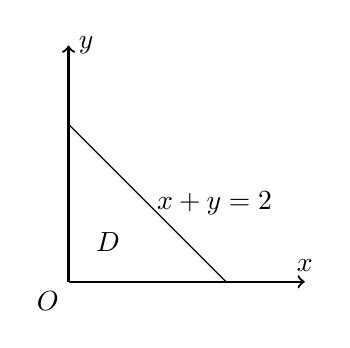
\begin{tikzpicture}
\draw[thick,->] (0,0) -> (3,0)node[above]{\(x\)};
\draw[thick,->] (0,0) -> (0,3)node[right]{\(y\)};
\draw (.5,.5)node{\(D\)};
\draw (0,0)node[below left]{\(O\)};
\draw (0,2)--(2,0)node[midway,right]{\(x+y=2\)};
\end{tikzpicture}
\subcaption{}
\end{subfigure}%
\begin{subfigure}[b]{\subwidth}
\centering
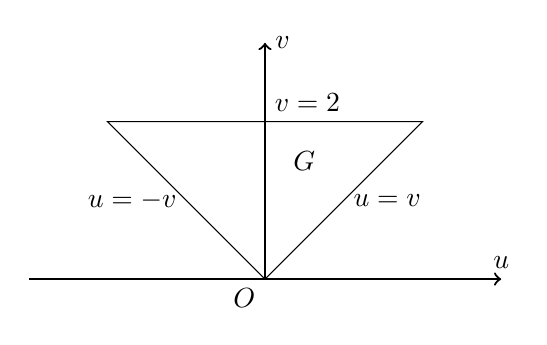
\begin{tikzpicture}
\draw[thick,->] (-3,0) -> (3,0)node[above]{\(u\)};
\draw[thick,->] (0,0) -> (0,3)node[right]{\(v\)};
\draw (.5,1.5)node{\(G\)};
\draw (0,0)node[below left]{\(O\)};
\draw (0,0)--(2,2)node[midway,right]{\(u=v\)}
    --(-2,2)node[midway,above right]{\(v=2\)}
    --(0,0)node[midway,left]{\(u=-v\)};
\end{tikzpicture}
\subcaption{}
\end{subfigure}%
\caption{}
\end{figure}

雅克比式为\[
J = \jacobi{x,y}{u,v}
= \def\arraystretch{1.5} \begin{vmatrix}
-\frac{1}{2} & \frac{1}{2} \\
\frac{1}{2} & \frac{1}{2}
\end{vmatrix}
= - \frac{1}{2}.
\]那么\begin{align*}
\iint_D \exp(\frac{y-x}{y+x}) \dd{x} \dd{y}
&= \iint_G e^{\frac{u}{v}} \abs{-\frac{1}{2}} \dd{u} \dd{v} \\
&= \frac{1}{2} \int_0^2 \dd{v} \int_{-v}^v e^{\frac{u}{v}} \dd{u} \\
&= \frac{1}{2} \int_0^2 \left( e - e^{-1} \right) v \dd{v}
= e - e^{-1}.
\end{align*}
\end{solution}
\end{example}

\begin{example}
计算\(\iint_D \sqrt{1 - \frac{x^2}{a^2} - \frac{y^2}{b^2}} \dd{x} \dd{y}\),
其中\(D\)是椭圆\(\frac{x^2}{a^2} + \frac{y^2}{b^2} = 1\ (a,b>0)\)所围成的闭区域.
\begin{solution}
作广义极坐标变换\[
\left\{ \begin{array}{l}
x = a \rho \cos\theta, \\
y = b \rho \sin\theta.
\end{array} \right.
\]
在这变换下,与\(D\)对应的闭区域为\(G = \Set{\opair{\rho,\theta} \given 0\leq\rho\leq1,0\leq\theta\leq2\pi}\),雅克比式\[
J = \jacobi{x,y}{\rho,\theta} = ab\rho.
\]由于\(J\)仅当\(\rho=0\)时为零,所以换元公式仍成立,从而有\[
\iint_D \sqrt{1 - \frac{x^2}{a^2} - \frac{y^2}{b^2}} \dd{x} \dd{y}
= \iint_G \sqrt{1-\rho^2} ab\rho \dd{\rho} \dd{\theta}
= \frac{2}{3} \pi ab.
\]
\end{solution}
\end{example}

\section{三重积分}
\subsection{三重积分的概念}
定积分及二重积分作为和的极限的概念,可以很自然地推广到三重积分.
\begin{definition}
设\(f(x,y,z)\)是空间有界闭区域\(\Omega\)上的有界函数.将\(\Omega\)任意分成\(n\)个小闭区域\[
\increment v_1,\, \increment v_2,\, \dotsc,\, \increment v_n,
\]其中\(\increment v_i\)表示第\(i\)个小闭区域,
也表示它的体积.在每个\(\increment v_i\)上任取一点\(\opair{\xi_i,\eta_i,\zeta_i}\),
作乘积\(f(\xi_i,\eta_i,\zeta_i) \increment v_i\ (i=1,2,\dotsc,n)\),
并作和\(\sum\limits_{i=1}^n f(\xi_i,\eta_i,\zeta_i) \increment v_i\).
如果当各小闭区域直径中的最大值\(\lambda\)趋于零时这和的极限总存在,
则称此极限为“函数\(f(x,y,z)\)在闭区域\(\Omega\)上的\DefineConcept{三重积分}(triple integral)”,
记作\(\iiint_{\Omega} f(x,y,z) \dd{v}\),即\[
\iiint_{\Omega} f(x,y,z) \dd{v}
= \lim\limits_{\lambda\to0} \sum\limits_{i=1}^n f(\xi_i,\eta_i,\zeta_i) \increment v_i,
\eqno{(1)}
\]其中\(\dd{v}\)叫做\DefineConcept{体积元素}.
\end{definition}

在直角坐标系中,如果用平行于坐标面的平面来划分\(\Omega\),那么除了包含\(\Omega\)的边界点的一些不规则小闭区域外,得到的小闭区域\(\increment v_i\)为长方体.设长方体小闭区域\(\increment v_i\)的边长为\(\increment x_j,\increment y_k,\increment z_l\),则\(\increment v_i = \increment x_j \increment y_k \increment z_l\).因为在直角坐标系中,有时也把体积元素\(\dd{v}\)记作\(\dd{x}\dd{y}\dd{z}\),而把三重积分记作\[
\iiint_{\Omega} f(x,y,z) \dd{x}\dd{y}\dd{z},
\]其中\(\dd{x}\dd{y}\dd{z}\)叫做\DefineConcept{直角坐标系中的体积元素}.

当函数\(f(x,y,z)\)在闭区域\(\Omega\)上连续时,(1)式右端的和的极限必定存在,也就是函数\(f(x,y,z)\)在闭区域\(\Omega\)上的三重积分必定存在.以后我们总假定函数\(f(x,y,z)\)在闭区域\(\Omega\)上是连续的.关于二重积分的一些术语,例如被积函数、积分区域等,也可相应地用到三重积分上.三重积分的性质也与第一节中所叙述的二重积分的性质相类似,这里不再重复了.

如果\(f(x,y,z)\)表示某物体在点\(\opair{x,y,z}\)处的密度,\(\Omega\)是该物体所占有的空间闭区域,\(f(x,y,z)\)在\(\Omega\)上连续,则\(\sum\limits_{i=1}^n f(\xi_i,\eta_i,\zeta_i) \increment v_i\)是该物体的质量\(m\)的近似值,这个和当\(\lambda\to0\)时的极限就是该物体的质量\(m\),所以\[
m = \iiint_{\Omega} f(x,y,z) \dd{v}.
\]

\subsection{三重积分的计算法}
计算三重积分的基本方法是将三重积分化为三次积分来计算.下面按利用不同的坐标来分别讨论将三重积分化为三次积分的方法,且只限于叙述方法.

\subsubsection{利用直角坐标系计算三重积分}
假设平行于\(z\)轴且穿过闭区域\(\Omega\)内部的直线与闭区域\(\Omega\)的边界曲面\(S\)相交不多于两点.把闭区域\(\Omega\)投影到\(xOy\)平面上,得一平面闭区域\(D_{xy}\).以\(D_{xy}\)为边界为准线作母线平行于\(z\)轴的柱面.这柱面与曲面\(S\)的交线从\(S\)中分出的上、下两部分,它们的方程分别为\begin{gather*}
S_1 : z = z_1(x,y), \\
S_2 : z = z_2(x,y),
\end{gather*}其中\(z_1(x,y)\)与\(z_2(x,y)\)都是\(D_{xy}\)上的连续函数,且\(z_1(x,y) \leq z_2(x,y)\).
过\(D_{xy}\)内任一点\(\opair{x,y}\)作平行于\(z\)轴的直线,这直线通过曲面\(S_1\)穿入\(\Omega\)内,然后通过曲面\(S_2\)穿出\(\Omega\)外,穿入点与穿出点的竖坐标分别为\(z_1(x,y)\)与\(z_2(x,y)\).

这种情况下,积分区域\(\Omega\)可表示为\[
\Omega = \Set{ \opair{x,y,z} \given z_1(x,y) \leq z \leq z_2(x,y) \land \opair{x,y} \in D_{xy} }.
\]

先将\(x,y\)看作固定值,将\(f(x,y,z)\)只看做\(z\)的函数,在区间\([z_1(x,y),z_2(x,y)]\)上对\(z\)积分.积分的结果是\(x\)、\(y\)的函数,记作\(F(x,y)\),即\[
F(x,y)=\int_{z_1(x,y)}^{z_2(x,y)} f(x,y,z) \dd{z}.
\]然后计算\(F(x,y)\)在闭区域\(D_{xy}\)上的二重积分\[
\iint_{D_{xy}} F(x,y) \dd{\sigma}
=\iint_{D_{xy}} \left[
 \int_{z_1(x,y)}^{z_2(x,y)} f(x,y,z) \dd{z}
\right] \dd{\sigma}.
\]假如闭区域\[
D_{xy} = \Set{ \opair{x,y} \given y_1(x) \leq y \leq y_2(x) \land a \leq x \leq b },
\]把这个二重积分化为二次积分,于是得到三重积分的计算公式\[
\iiint_{\Omega} f(x,y,z) \dd{v}
= \int_a^b  \dd{x} \int_{y_1(x)}^{y_2(x)} \dd{y} \int_{z_1(x,y)}^{z_2(x,y)} f(x,y,z) \dd{z}.
\eqno{(2)}
\]公式(2)把三重积分化为先对\(z\)、再对\(y\)、最后对\(x\)的三次积分.

如果平行于\(x\)轴或\(y\)轴且穿过闭区域\(\Omega\)内部的直线与\(\Omega\)的边界曲面\(S\)相交不多于两点,也可把闭区域\(\Omega\)投影到\(yOz\)面上或\(xOz\)面上,这样便可把三重积分化为按其他顺序的三次积分.如果平行于坐标轴且穿过闭区域\(\Omega\)内部的直线与边界曲面\(S\)的交点多于两个,也可像处理二重积分那样,把\(\Omega\)分成若干部分,使\(\Omega\)上的三重积分化为各部分闭区域上的三重积分的和.

\begin{example}
计算三重积分\(\iiint_{\Omega} x \dd{x}\dd{y}\dd{z}\),其中\(\Omega\)是三个坐标面及平面\(x+2y+z=1\)所围成的闭区域.
\begin{solution}
将\(\Omega\)投影到\(xOy\)面上,得投影区域\(D_{xy}\)为三角形闭区域\[
D_{xy} = \Set{ \opair{x,y} \given 0 \leq \frac{1-x}{2}, 0 \leq x \leq 1 }.
\]

在\(D_{xy}\)内任取一点\(\opair{x,y}\),过此点作平行于\(z\)轴的直线,该直线通过平面\(z = 0\)穿入\(\Omega\)内,然后通过平面\(z = 1 - x - 2y\)穿出\(\Omega\)外.于是由公式(2)得\begin{align*}
\iiint_{\Omega} x \dd{x}\dd{y}\dd{z}
&= \int_0^1 \dd{x} \int_0^{(1-x)/2} \dd{y} \int_0^{1-x-2y} x \dd{z} \\
&= \int_0^1 x \dd{x} \int_0^{(1-x)/2} (1-x-2y) \dd{y} \\
&= \frac{1}{4} \int_0^1 (x - 2x^2 + x^3) \dd{x}
= \frac{1}{48}.
\end{align*}
\end{solution}
\end{example}

有时,我们计算一个三重积分也可以化为先计算一个二重积分、再计算一个定积分,即有下述计算公式.

设空间闭区域\[
\Omega = \Set{ \opair{x,y,z} \given c_1 \leq z \leq c_2 \land \opair{x,y} \in D_z },
\]其中\(D_z\)是竖坐标为\(z\)的平面截空间闭区域\(\Omega\)所得到的一个平面闭区域,则有\[
\iiint_{\Omega} f(x,y,z) \dd{v}
=\int_{c_1}^{c_2} \dd{z} \iint_{D_{z}} f(x,y,z) \dd{x}\dd{y}.
\eqno{(3)}
\]

\begin{example}
计算三重积分\(\iiint_{\Omega} z^2 \dd{x}\dd{y}\dd{z}\),其中\(\Omega\)是由椭球面\(\frac{x^2}{a^2}+\frac{y^2}{b^2}+\frac{z^2}{c^2}=1\)所围成的空间闭区域.
\begin{solution}
空间闭区域\(\Omega\)可表示为\[
\Set*{ \opair{x,y,z} \given \frac{x^2}{a^2}+\frac{y^2}{b^2}\leq1-\frac{z^2}{c^2}, -c \leq z \leq c }.
\]由公式(3)得\[
\iiint_{\Omega} z^2 \dd{x}\dd{y}\dd{z}
= \int_{-c}^c z^2 \dd{z} \iint_{D_z} \dd{x}\dd{y} = \pi ab \int_{-c}^c \left(1-\frac{z^2}{c^2}\right) z^2 \dd{z} = \frac{4}{15}\pi abc^3.
\]
\end{solution}
\end{example}

\subsubsection{利用柱面坐标系计算三重积分}
利用以下关系\[
\left\{ \begin{array}{l}
x = \rho\cos\theta \\
y = \rho\sin\theta \\
z = z \\
\end{array} \right.
\]替换三重积分\(\iiint_{\Omega}{f(x,y,z)\dd{x}\dd{y}\dd{z}}\)中的积分变量,即有\[
\iiint_{\Omega}{f(x,y,z)\dd{x}\dd{y}\dd{z}}
= \iiint_{\Omega}{f(\rho \cos\theta,\rho \sin\theta,z) \rho \dd{\rho} \dd{\theta} \dd{z}},
\]其中,\(\dd{v} = \rho \dd{\rho} \dd{\theta} \dd{z}\)称为\DefineConcept{柱面坐标系中的体积元素}.

\subsubsection{利用球面坐标系计算三重积分}
利用以下关系\[
\left\{ \begin{array}{l}
x = r \sin\varphi \cos\theta, \\
y = r \sin\varphi \sin\theta, \\
z = r \cos\varphi
\end{array} \right.
\]替换三重积分\(\iiint_{\Omega}{f(x,y,z)\dd{x}\dd{y}\dd{z}}\)中的积分变量,即有\[
\iiint_{\Omega}{f(x,y,z)\dd{x}\dd{y}\dd{z}}
= \iiint_{\Omega}{f(r \sin\varphi \cos\theta,r \sin\varphi \sin\theta,r \cos\varphi) r^2 \sin\varphi \dd{r} \dd{\varphi} \dd{\theta}},
\]其中,\(\dd{v} = r^2 \sin\varphi \dd{r} \dd{\varphi} \dd{\theta}\)称为\DefineConcept{球面坐标系中的体积元素}.

\begin{example}
证明:半径为\(R\)的球的体积为\(V = \frac{4}{3} \pi R^3\).
\begin{proof}
以球心为原点建立球面坐标系,得球的方程为\[
\Omega: r \leq R.
\]那么球的体积为\begin{align*}
V &= \iiint_{\Omega} r^2 \sin\varphi \dd{r} \dd{\varphi} \dd{\theta} \\
&= \int_0^R r^2 \dd{r} \int_0^{\pi} \sin\varphi \dd{\varphi} \int_0^{2\pi} \dd{\theta} \\
&= \frac{1}{3} R^3 \cdot 2 \cdot 2\pi
= \frac{4}{3} \pi R^3.
\qedhere
\end{align*}
\end{proof}
\end{example}

\section{扩展:多重积分的一般性理论}
\subsection{重积分化为累次积分}
\begin{theorem}[富比尼定理]
设区域\(X\subseteq\mathbb{R}^m, Y\subseteq\mathbb{R}^n\).
如果函数\(f\colon X \times Y \to \mathbb{R}\)在\(X \times Y\)上可积,则\(f\)的重积分与累次积分同时存在且彼此相等,即\[
\int_{X \times Y} f(x,y) \dd{x}\dd{y}
= \int_X \dd{x} \int_Y f(x,y) \dd{y}
= \int_Y \dd{y} \int_X f(x,y) \dd{x}.
\]
\end{theorem}

\begin{corollary}
如果函数\(f\in\mathcal{R}(X \times Y)\),则(在勒贝格意义下)%
对于几乎所有的值\(x \in X\),积分\(\int_Y f(x,y) \dd{y}\)存在;%
对于几乎所有的值\(y \in Y\),积分\(\int_X f(x,y) \dd{x}\)存在.
\end{corollary}

\begin{corollary}
\newcommand\intx[2][]{\int_{a_{#2}}^{b_{#2}} #1 \dd{x_{#2}}}%
如果区间\(I \subseteq \mathbb{R}^n\)是闭区域\(I_i = [a_i,b_i]\ (i=1,2,\dotsc,n)\)的直积,则\[
	\int_I f(x) \dd{x}
	= \intx{n} \intx{n-1} \dotso \intx[f(\AutoTuple{x}{n})]{1}.
\]
\end{corollary}

\subsection{重积分中的变量代换}
利用雅克比式,可以把二重积分的换元法推广到多元函数上.
\begin{theorem}
若连续可微函数\[
	\mat{y} = f(\mat{x})
	\quad(\mat{x},\mat{y}\in\mathbb{R}^n)
\]
把\(O x_1 x_2 \dotso x_n\)空间(新坐标空间)内的有界闭区域\(\Omega\)
单值地映射成\(O' y_1 y_2 \dotso y_n\)空间(旧坐标空间)内的有界闭区域\(\Omega'\),
并且在闭区域\(\Omega'\)内雅克比行列式\[
	J = \det\mat{J}
	= \jacobi{f_1,f_2,\dotsc,f_n}{\AutoTuple{x}{n}}
	= { \def\arraystretch{1.5} \begin{vmatrix}
		\pdv{f_1}{x_1} & \pdv{f_1}{x_2} & \dots & \pdv{f_1}{x_n} \\
		\pdv{f_2}{x_1} & \pdv{f_2}{x_2} & \dots & \pdv{f_2}{x_n} \\
		\vdots & \vdots & & \vdots \\
		\pdv{f_n}{x_1} & \pdv{f_n}{x_2} & \dots & \pdv{f_n}{x_n} \\
	\end{vmatrix} }
	\neq 0,
\]
则有如下的积分换元公式\begin{equation}
\begin{split}
	&\idotsint\limits_{\Omega'}
		F(\AutoTuple{y}{n})
		\dd{y_1}\dd{y_2}\dotsm\dd{y_n} \\
	&\hspace{20pt}=
		\idotsint\limits_\Omega
		F(\AutoTuple{x}{n})
		\abs{J}
		\dd{x_1}\dd{x_2}\dotsm\dd{x_n}.
\end{split}
\end{equation}
\end{theorem}
利用上述积分换元公式可以将复杂的被积函数化简,也可以将复杂的积分区域化为更具对称性的积分区域.


\section{重积分的应用}
\subsection{利用重积分的定义计算极限}
\begin{example}
用二重积分的定义计算极限\[
\lim\limits_{n\to\infty} \sum\limits_{i=1}^n \sum\limits_{j=1}^n \frac{n}{(n+i)(n^2+j^2)}.
\]
\begin{solution}
首先观察极限\begin{align*}
	&\hspace{-20pt}
	\lim\limits_{n\to\infty}
		\sum\limits_{i=1}^n
		\sum\limits_{j=1}^n \frac{n}{(n+i)(n^2+j^2)} \\
	&= \lim\limits_{n\to\infty}
		\sum\limits_{i=1}^n
		\sum\limits_{j=1}^n \frac{1}{n^2} \frac{n^3}{(n+i)(n^2+j^2)} \\
	&= \lim\limits_{n\to\infty}
		\sum\limits_{i=1}^n
		\sum\limits_{j=1}^n \frac{1}{n^2}
		\left[
			\left(1+\frac{i}{n}\right)
			\left(1+\frac{j^2}{n^2}\right)
		\right]^{-1},
\end{align*}
考虑当\(i=j=1\)时,\(\frac{i}{n},\frac{j}{n}\to0\ (n\to\infty)\);
当\(i=j=n\)时,\(\frac{i}{n}=\frac{j}{n}=1\);
那么可以将所求极限视作函数\(\frac{1}{1+x}\cdot\frac{1}{1+y^2}\)
在区域\([0,1]\times[0,1]\)上的积分\[
	\int_0^1 \dd{x} \int_0^1 \frac{1}{(1+x)(1+y^2)} \dd{y}
	= \int_0^1 \frac{1}{1+x} \dd{x} \int_0^1 \frac{1}{1+y^2} \dd{y}.
\]
\end{solution}
\end{example}

\subsection{曲面的面积}
设两平面\(\Pi_1\)、\(\Pi_2\)的夹角为\(\theta\ (0<\theta<\pi/2)\)
(如\cref{figure:重积分.平面区域的投影}),
\(\Pi_1\)上的闭区域\(D\)在\(\Pi_2\)上的投影区域为\(D_0\),
则\(D\)的面积\(A\)与\(D_0\)的面积\(\sigma\)满足\[
	A = \frac{\sigma}{\cos\theta}.
\]
事实上,先假定\(D\)是矩形闭区域,
且其一边平行于平面\(\Pi_1\)、\(\Pi_2\)的交线\(l\),
两条边的边长分别为\(a\)、\(b\),则\(D_0\)也是矩形闭区域,
且边长分别为\(a\)、\(b \cos\theta\),从而\[
	\sigma = ab\cos\theta = A \cos\theta.
\]

\begin{figure}[ht]
	\centering
	\begin{tikzpicture}[scale=2]
		\draw[name path=upper](0,0)--++(1,-1)node[midway,below left]{\(l\)}coordinate(p1)
			--++(2,2)coordinate(p2)
			--++(-1,1)node[below]{\(\Pi_1\)}
			--++(-2,-2);
		\path[name path=horizon](1,0)--++(2,0);
		\draw[name intersections={of=upper and horizon},dashed]
			(intersection-1)--(0,0);
		\draw(p1)--++(3,0)coordinate(p3)
			--++(-1,1)node[below]{\(\Pi_2\)}
			--(intersection-1);
		\draw pic["\(\theta\)",draw=orange,-,angle eccentricity=2,angle radius=0.3cm]{angle=p3--p1--p2};
		\draw(1.6,.9)coordinate(A)
			--++(.3,-.3)coordinate(B)node[midway,below left]{\(a\)}
			--++(.2,.2)coordinate(C)node[midway,below right]{\(b\)}
			--++(-.3,.3)coordinate(D)
			--++(-.2,-.2);
		\begin{scope}[dashed]
		\draw(A)--++(0,-1.4)coordinate(A1);
		\draw(B)--++(0,-1.4)coordinate(B1);
		\draw(C)--++(0,-1.4-.2)coordinate(C1);
		\draw(D)--++(0,-1.4-.2)coordinate(D1);
		\end{scope}
		\draw(A1)--(B1)node[midway,below left]{\(a\)}--(C1)node[midway,below]{\(b \cos\theta\)}--(D1)--(A1);
	\end{tikzpicture}
	\caption{平面区域的投影}
	\label{figure:重积分.平面区域的投影}
\end{figure}

\begin{theorem}
设曲面\(S\)由方程\[
z=f(x,y)
\]给出,\(D_{xy}\)为曲面\(S\)在\(xOy\)面上的投影区域,
函数\(f(x,y)\)在\(D_{xy}\)上具有连续偏导数\(f'_x(x,y)\)和\(f'_y(x,y)\).
那么曲面\(S\)面积元素\(\dd{A}\)为\[
\dd{A} = \sqrt{1 + [f'_x(x,y)]^2 + [f'_y(x,y)]^2} \dd{\sigma}.
\]

曲面\(S\)的面积为\begin{align}
A &= \iint_{D_{xy}} \sqrt{1 + [f'_x(x,y)]^2 + [f'_y(x,y)]^2} \dd{\sigma} \nonumber \\
&= \iint_{D_{xy}} \sqrt{1 + \left(\pdv{z}{x}\right)^2 + \left(\pdv{z}{y}\right)^2} \dd{x}\dd{y}.
\end{align}
\end{theorem}

设曲面的方程为\(x=g(y,z)\)或\(y=h(z,x)\),
可分别把曲面投影到\(yOz\)面上(投影区域记作\(D_{yz}\))或\(zOx\)面上(投影区域记作\(D_{zx}\)),
类似地可得\begin{equation}
A = \iint_{D_{yz}} \sqrt{1 + \left(\pdv{x}{y}\right)^2 + \left(\pdv{x}{z}\right)^2} \dd{y}\dd{z},
\end{equation}或\begin{equation}
A = \iint_{D_{zx}} \sqrt{1 + \left(\pdv{y}{z}\right)^2 + \left(\pdv{y}{x}\right)^2} \dd{z}\dd{x}.
\end{equation}

\begin{example}
求半径为\(R\)的球的表面积.
\begin{solution}
\def\z{\sqrt{R^2-x^2-y^2}}
取上半球面方程为\(z = \z\),则它在\(xOy\)面上的投影区域为\[
D = \Set{\opair{x,y} \given x^2+y^2 \leq R^2}.
\]由\[
\pdv{z}{x} = \frac{-x}{\z},
\qquad
\pdv{z}{y} = \frac{-y}{\z},
\]得\[
\sqrt{1 + \left(\pdv{y}{z}\right)^2 + \left(\pdv{y}{x}\right)^2}
= \frac{R}{\z}.
\]因为这函数在闭区域\(D\)上无界,我们不能直接应用曲面面积公式,所以先取区域\[
D_1 = \Set{\opair{x,y} \given x^2+y^2 \leq r^2}
\quad(0<r<R)
\]为积分区域,算出相应于\(D_1\)上的球面面积\[
A_1 = \iint_{D_1} \frac{R}{\z} \dd{x}\dd{y}
\]后,令\(r \to R\)取\(A_1\)的极限就得半球面的面积.

\def\zz{\sqrt{R^2-\rho^2}}
利用极坐标,得\[
A_1 = \iint_{D_1} \frac{R}{\zz} \rho\dd{\rho}\dd{\theta}
= R \int_0^{2\pi} \dd{\theta} \int_0^r \frac{\rho \dd{\rho}}{\zz}
= 2\pi R(R-\sqrt{R^2-r^2}),
\]
\def\l{\lim\limits_{r \to R}}
于是\begin{equation}
A = \l A_1
= \l 2\pi R(R-\sqrt{R^2-r^2})
= 2\pi R^2.
\end{equation}
\end{solution}
\end{example}

\begin{theorem}[利用曲面的参数方程求曲面的面积]
设曲面\(S\)由参数方程\[
\left\{ \begin{array}{l}
x = x(u,v), \\
y = y(u,v), \\
z = z(u,v) \\
\end{array} \right.
\quad
\opair{u,v} \in D
\]给出,其中\(D\)是一个平面有界闭区域,又\(x(u,v), y(u,v), z(u,v)\)在\(D\)上具有连续的一阶偏导数,且\[
\jacobi{x,y}{u,v}, \qquad
\jacobi{y,z}{u,v}, \qquad
\jacobi{z,x}{u,v}
\]不全为零,则曲面\(S\)的面积为
\begin{equation}\label{equation:重积分.曲面的面积计算公式}
A = \iint_D \sqrt{E G - F^2} \dd{u}\dd{v},
\end{equation}其中\begin{align*}
E &= (x'_u)^2 + (y'_u)^2 + (z'_u)^2, \\
F &= x'_u \cdot x'_v + y'_u \cdot y'_v + z'_u \cdot z'_v, \\
G &= (x'_v)^2 + (y'_v)^2 + (z'_v)^2.
\end{align*}
\rm
上述\(E\)、\(F\)和\(G\)又称为曲面的\DefineConcept{高斯系数}.
\end{theorem}
\begingroup
\def\J{\mat{J}}%
\cref{equation:重积分.曲面的面积计算公式} 也可记作\[
A = \iint_D \sqrt{\det(\J^T \J)} \dd{u}\dd{v},
\]其中雅克比矩阵\[
\J = \begin{bmatrix}
x'_u & x'_v \\
y'_u & y'_v \\
z'_u & z'_v
\end{bmatrix}.
\]
\endgroup

\subsection{物体的质心}
\begin{theorem}
设物体占有空间有界闭区域\(\Omega\),其在点\(\opair{x,y,z}\)处的密度为\[
\rho=\rho(x,y,z)
\](假定\(\rho(x,y,z)\)在\(\Omega\)上连续),则其质心坐标为\begin{equation}
\opair*{
\frac{1}{M} \iiint_{\Omega} x \rho \dd{v},
\frac{1}{M} \iiint_{\Omega} y \rho \dd{v},
\frac{1}{M} \iiint_{\Omega} z \rho \dd{v}
}
\end{equation}其中\(M = \iiint_{\Omega} \rho \dd{v}\).
\end{theorem}

\subsection{物体的转动惯量}
\begin{theorem}
设物体占有空间有界闭区域\(\Omega\),其在点\(\opair{x,y,z}\)处的密度为\[
\rho=\rho(x,y,z)
\](假定\(\rho(x,y,z)\)在\(\Omega\)上连续),则其相对于\(x\)、\(y\)、\(z\)轴的转动惯量为\begin{align}
I_x &= \iiint_{\Omega} (y^2+z^2) \rho(x,y,z) \dd{v}, \\
I_y &= \iiint_{\Omega} (z^2+x^2) \rho(x,y,z) \dd{v}, \\
I_z &= \iiint_{\Omega} (x^2+y^2) \rho(x,y,z) \dd{v}.
\end{align}
\end{theorem}

\subsection{引力}
\begin{theorem}
设引力常量为\(G\),物体占有空间有界闭区域\(\Omega\),它在点\(\opair{x,y,z}\)处的密度为\[
\rho=\rho(x,y,z),
\]并假定\(\rho(x,y,z)\)在\(\Omega\)上连续,则其对物体外一点\(P_0(x_0,y_0,z_0)\)的引力为\begin{equation}
\mat{F}
= \opair*{
G \cdot \iiint_{\Omega} \frac{\rho (x-x_0)}{r^3} \dd{v},
G \cdot \iiint_{\Omega} \frac{\rho (y-y_0)}{r^3} \dd{v},
G \cdot \iiint_{\Omega} \frac{\rho (z-z_0)}{r^3} \dd{v}
}.
\end{equation}
\end{theorem}

\section{含参变量的积分}
\subsection{含参变量积分的概念与性质}
设\(f(x,y)\)是矩形(闭区域)\(R = [a,b]\times[c,d]\)上的连续函数.
在\([a,b]\)上任意取定\(x\)的一个值,于是\(f(x,y)\)是变量\(y\)在\([c,d]\)上的一个一元连续函数,从而积分\[
\int_c^d f(x,y) \dd{y}
\]存在,这个积分的值依赖于取定的\(x\)的值.
当\(x\)的值改变时,一般来说这个积分的值也跟着改变.
这个积分确定一个定义在\([a,b]\)上的关于\(x\)的函数,若将其记为\(\varphi(x)\),则有\[
\varphi(x) = \int_c^d f(x,y) \dd{y}
\quad(a \leq x \leq b).
\]这里变量\(x\)在积分过程中看作是一个常量,通常称其为\DefineConcept{参变量},因此上式右端是一个含参变量\(x\)的积分,这个积分确定关于\(x\)的一个函数\(\varphi(x)\).
下面讨论关于\(\varphi(x)\)的一些性质.

\begin{theorem}
如果函数\(f(x,y)\)在矩形\(R=[a,b]\times[c,d]\)上连续,
那么函数\[
\varphi(x) = \int_c^d{f(x,y)\dd{y}}, \quad a \leq x \leq b
\]在\([a,b]\)上也连续.
\end{theorem}

\begin{theorem}
如果函数\(f(x,y)\)在矩形\(R=[a,b]\times[c,d]\)上连续,则\[
\int_a^b\left[\int_c^d f(x,y) \dd{y}\right] \dd{x}
=\int_c^d\left[\int_a^b f(x,y) \dd{x}\right] \dd{y}.
\]
\end{theorem}
上式也可写成\[
\int_a^b \dd{x} \int_c^d f(x,y) \dd{y}
=\int_c^d \dd{y} \int_a^b f(x,y) \dd{x}.
\]

\begin{theorem}
如果函数\(f(x,y)\)及其偏导数\(f'_x(x,y)\)都在矩形\(R=[a,b]\times[c,d]\)上连续,那么函数\[
\varphi(x) = \int_c^d f(x,y) \dd{y}
\quad(a \leq x \leq b)
\]在\([a,b]\)上可微,并且\[
\varphi'(x) = \dv{x} \int_c^d f(x,y) \dd{y}
= \int_c^d f'_x(x,y) \dd{y}.
\]
\end{theorem}

\begin{theorem}
如果函数\(f(x,y)\)在矩形\(R=[a,b]\times[c,d]\)上连续,
函数\(\alpha(x)\)与\(\beta(x)\)在区间\([a,b]\)上连续,且\[
x \in [a,b] \implies \alpha(x),\beta(x) \in [c,d],
\]则函数\[
\Phi(x) = \int_{\alpha(x)}^{\beta(x)} f(x,y)\dd{y}
\quad(a \leq x \leq b)
\]在\([a,b]\)上也连续.
\end{theorem}

\begin{theorem}
如果函数\(f(x,y)\)及其偏导数\(f'_x(x,y)\)都在矩形\(R=[a,b]\times[c,d]\)上连续,
函数\(\alpha(x)\)与\(\beta(x)\)在区间\([a,b]\)上可微,且\[
x \in [a,b] \implies \alpha(x),\beta(x) \in [c,d],
\]则函数\[
\Phi(x) = \int_{\alpha(x)}^{\beta(x)} f(x,y)\dd{y}
\quad(a \leq x \leq b)
\]在\([a,b]\)上也可微,且\begin{align*}
\Phi'(x) &= \dv{x} \int_{\alpha(x)}^{\beta(x)} f(x,y) \dd{y} \\
&= \int_{\alpha(x)}^{\beta(x)} f'_x(x,y) \dd{y}
	+ f[x,\beta(x)] \cdot \beta'(x)
	- f[x,\alpha(x)] \cdot \alpha'(x).
\end{align*}
\end{theorem}
上式也被称为\DefineConcept{莱布尼茨公式}.

\begin{example}
设\(F(x) = \int_x^{x^2} \frac{\sin xy}{y} \dd{y}\),求\(F'(x)\).
\begin{solution}
应用莱布尼茨公式,得\begin{align*}
F'(x) &= \int_x^{x^2} \cos xy \dd{y}
+ \frac{\sin x^3}{x^2} \cdot 2x
- \frac{\sin x^2}{x} \cdot 1 \\
&= \left[ \frac{\sin xy}{x} \right]_x^{x^2}
+ \frac{2 \sin x^3}{x}
- \frac{\sin x^2}{x}
= \frac{3 \sin x^3 - 2 \sin x^2}{x}.
\end{align*}
\end{solution}
\end{example}

\begin{example}
求\(I = \int_0^1 \frac{x^b-x^a}{\ln x} \dd{x}\ (0<a<b)\).
\begin{solution}
因为\[
\int_a^b x^y \dd{y}
= \left[ \frac{x^y}{\ln x} \right]_a^b
= \frac{x^b - x^a}{\ln x},
\]所以\[
I = \int_0^1 \dd{x} \int_a^b x^y \dd{y}.
\]这里函数\(f(x,y) = x^y\)在矩形\(R=[0,1]\times[a,b]\)上连续,那么只要交换积分次序,就有\[
I = \int_a^b \dd{y} \int_0^1 x^y \dd{x}
= \int_a^b \left[\frac{x^{y+1}}{y+1}\right]_0^1 \dd{y}
= \int_a^b \frac{1}{y+1} \dd{y}
= \ln\frac{b+1}{a+1}.
\]
\end{solution}
\end{example}

\begin{example}
计算定积分\(I = \int_0^1 \frac{\ln(1+x)}{1+x^2} \dd{x}\).
\begin{solution}
考虑含参变量\(\alpha\)的积分所确定的函数\[
\varphi(\alpha) = \int_0^1 \frac{\ln(1+\alpha x)}{1+x^2} \dd{x}.
\]显然,\(\varphi(0) = 0\),\(\varphi(1) = I\).
对\(\varphi(\alpha)\)求导得\[
\varphi'(\alpha)
= \int_0^1 \frac{x}{(1+\alpha x)(1+x^2)} \dd{x}.
\]把被积函数分解为部分分式,得到\[
\frac{x}{(1+\alpha x)(1+x^2)}
= \frac{1}{1+\alpha^2} \left[
\frac{-\alpha}{1+\alpha x}
+ \frac{x}{1+x^2}
+ \frac{\alpha}{1+x^2}
\right].
\]于是\begin{align*}
\varphi'(\alpha)
&= \frac{1}{1+\alpha^2} \left[
\int_0^1 \frac{-\alpha \dd{x}}{1+\alpha x}
+ \int_0^1 \frac{x \dd{x}}{1+x^2}
+ \int_0^1 \frac{\alpha \dd{x}}{1+x^2}
\right] \\
&= \frac{1}{1+\alpha^2} \left[
-\ln(1+\alpha)
+ \frac{1}{2} \ln2
+ \alpha \cdot \frac{\pi}{4}
\right],
\end{align*}
上式在\([0,1]\)上对\(\alpha\)积分,得到\begin{align*}
I &= \varphi(1)-\varphi(0)
= \int_0^1 \varphi'(\alpha) \dd{\alpha} \\
&= - \int_0^1 \frac{\ln(1+\alpha)}{1+\alpha^2} \dd{\alpha}
+ \frac{1}{2} \ln2 \int_0^1 \frac{\dd{\alpha}}{1+\alpha^2}
+ \frac{\pi}{4} \int_0^1 \frac{\alpha}{1+\alpha^2} \dd{\alpha} \\
&= -I + \frac{\ln2}{2} \cdot \frac{\pi}{4} + \frac{\pi}{4}\cdot\frac{\ln2}{2}
= -I + \frac{\pi}{4} \ln2,
\end{align*}
解得\(I = \frac{\pi}{8} \ln2\).
\end{solution}
\end{example}

\begin{example}
求函数\(f(x) = \int_1^{x^2} (x^2-t) e^{-t^2} \dd{t}\)的单调区间与极值.
\begin{solution}
求导得\[
\dv{f}{x}
= \int_1^{x^2} \pdv{x} (x^2-t) e^{-t^2} \dd{t}
= 2x \int_1^{x^2} e^{-t^2} \dd{t}.
\]
因为\(e^{-t^2}>0\ (-\infty<t<+\infty)\),所以根据\cref{theorem:定积分.定积分性质5},当\(x^2>1\)时,有\[
\int_1^{x^2} e^{-t^2} \dd{t} > 0;
\]当\(x^2 \leq 1\)时,有\[
\int_1^{x^2} e^{-t^2} \dd{t} \leq 0.
\]那么\begin{center}
\begin{tabular}{c|*7c}
\hline
\(x\) & \((-\infty,-1)\) & \(-1\) & \((-1,0)\) & \(0\) & \((0,1)\) & \(1\) & \((1,+\infty)\) \\ \hline
\(f'(x)\) & \(-\) & \(0\) & \(+\) & \(0\) & \(-\) & \(0\) & \(+\) \\
\(f(x)\) & \(\searrow\) & \(0\) & \(\nearrow\) & \((1-e^{-1})/2\) & \(\searrow\) & \(0\) & \(\nearrow\) \\
\hline
\end{tabular}
\end{center}
也就是说,函数\(f\)在区间\((-\infty,-1)\cup(0,1)\)上单调减少,在区间\((-1,0)\cup(1,+\infty)\)上单调增加,在点\(\pm1\)处取得极小值\(0\),在点\(0\)处取得极大值\(\frac{1-e^{-1}}{2}\).
\end{solution}
\end{example}
本例若利用\cref{theorem:定积分.定积分性质1} 将\[
\int_1^{x^2} (x^2-t) e^{-t^2} \dd{t}
\]拆开成\[
x^2 \int_1^{x^2} e^{-t^2} \dd{t}
\quad\text{和}\quad
\int_1^{x^2} t e^{-t^2} \dd{t}
\]两个部分,再分别对\(x\)求导,也可以求出\(\dv{f}{x}\).

\begin{example}%《高等数学(第六版 下册)》习题10-5 1.(1)
\def\l{\lim\limits_{x\to0}}%
计算极限\(\l \int_x^{x+1} \frac{\dd{y}}{1+x^2+y^2}\).
\begin{solution}
记\[
f(t) = \int_x^{x+t} \frac{\dd{y}}{1+x^2+y^2},
\]求导得\begin{align*}
f'(t)
&= \int_x^{x+t} \pdv{t}(\frac{1}{1+x^2+y^2}) \dd{y}
+ \frac{1}{1+x^2+(x+t)^2} \cdot 1
- \frac{1}{1+x^2+x^2} \cdot 0 \\
&= \frac{1}{1+x^2+(x+t)^2}.
\end{align*}
因为\(f(0) = 0\),所以
\begin{align*}
&\hspace{-20pt}
\l \int_x^{x+1} \frac{\dd{y}}{1+x^2+y^2} \\
&= f(1) - f(0)
= \int_0^1 f'(t) \dd{t} \\
&= \int_0^1 \frac{\dd{t}}{1+x^2+(x+t)^2} \\
&= \frac{1}{\sqrt{1+x^2}} \int_0^1 \left[1+\frac{(x+t)^2}{1+x^2}\right]^{-1} \dd(\frac{x+t}{\sqrt{1+x^2}}) \\
&= \frac{1}{\sqrt{1+x^2}} \left(\arctan\frac{x+t}{\sqrt{1+x^2}}\right)_0^1 \\
&= \frac{1}{\sqrt{1+x^2}} \left(
\arctan\frac{x+1}{\sqrt{1+x^2}}
- \arctan\frac{x}{\sqrt{1+x^2}}
\right).
\end{align*}
因此\[
\l \int_x^{x+1} \frac{\dd{y}}{1+x^2+y^2}
= \l f(1)
= \l \frac{1}{\sqrt{1+x^2}} \left(
\arctan\frac{x+1}{\sqrt{1+x^2}}
- \arctan\frac{x}{\sqrt{1+x^2}}
\right)
= \frac{\pi}{4}.
\]
\end{solution}
\end{example}

\begin{example}%《高等数学(第六版 下册)》习题10-5 1.(2)
\def\l{\lim\limits_{x\to0}}%
计算极限\(\l \int_{-1}^1 \sqrt{x^2+y^2} \dd{y}\).
\begin{solution}
设\[
f(t)
=\frac{1}{2} \int_{-t}^t \sqrt{x^2+y^2} \dd{y}
=\int_0^t \sqrt{x^2+y^2} \dd{y},
\]
求导得\[
f'(t)
= \int_0^t \pdv{t} \sqrt{x^2+y^2} \dd{y}
	+ \sqrt{x^2+t^2} \cdot 1
= \sqrt{x^2+t^2}.
\]又因为\(f(0) = 0\),所以\begin{align*}
\frac{1}{2} \int_{-1}^1 \sqrt{x^2+y^2} \dd{t}
&=f(1) - f(0)
= \int_0^1 f'(t) \dd{t}
= \int_0^1 \sqrt{x^2+t^2} \dd{t} \\
&= \left[
\frac{t}{2} \sqrt{x^2+t^2} + \frac{x^2}{2} \ln(t+\sqrt{x^2+t^2})
\right]_0^1 \\
&= \frac{1}{2} \sqrt{x^2+1} + \frac{x^2}{2} \left[ \ln(1+\sqrt{x^2+1}) - \ln\abs{x} \right]
\end{align*}
从而\[
\l \int_{-1}^1 \sqrt{x^2+y^2} \dd{y}
= \l \left[
\sqrt{x^2+1}
+ x^2 \ln(1+\sqrt{x^2+1}) - x^2 \ln\abs{x}
\right]
= 1.
\]
\end{solution}
\end{example}

之前我们讲到,在计算反常积分时,
可以直接利用反常积分的定义
以及牛顿--莱布尼茨公式.
除此以外,我们还可以从含参变量积分的思路处理复杂的反常积分问题.

\begin{example}
证明反常积分\[
I = \int_0^{+\infty} \frac{\sin x}{x} \dd{x}
\]收敛,并计算它的值.
\begin{proof}
令\(I(a) = \int_0^{+\infty} \frac{\sin x}{x} e^{-ax} \dd{x}\ (a>0)\),
于是\(I(0) = I\).
求导得\[
	I'(a) = \dv{a} I(a)
	= \int_0^{+\infty} \frac{\sin x}{x} e^{-ax} (-x) \dd{x}
	= - \int_0^{+\infty} e^{-ax} \sin x \dd{x}
	= - \frac{1}{a^2+1},
\]
再积分得\[
	I(a) = -\arctan a + C,
\]
其中\(C\)是待定常数.
令\(a\to+\infty\),
得\(\arctan a\to\frac{\pi}{2}\),
\(\int_0^{+\infty} \frac{\sin x}{x} e^{-ax} \dd{x} \to 0\),
所以\(C = \frac{\pi}{2}\).
因此\(I = I(0) = \frac{\pi}{2}\).
\end{proof}
\end{example}
上述反常积分又称为狄利克雷积分,利用留数定理也可以求出它的值.
%重积分

\chapter{曲线积分与曲面积分}
上一章已经把积分概念从积分范围为数轴上一个区间的情形推广到积分范围为平面或空间内的一个闭区域的情形.
本章将把积分概念推广到积分范围为一段具有有限长度的曲线弧或一片具有有限面积的曲面的情形(这样推广后的积分称为曲线积分或曲面积分),并阐明有关这两种积分的一些基本内容.

\section{对弧长的曲线积分}
\subsection{对弧长的曲线积分的概念}
\begin{definition}
设\(L\)为\(xOy\)面内一条光滑曲线弧,函数\(f(x,y)\)在\(L\)上有界.
在\(L\)上任意插入一点列\(M_1,M_2,\dotsc,M_{n-1}\)把\(L\)分成\(n\)个小段.
设第\(i\)个小段的长度为\(\increment s_i\).
又\(\opair{\xi_i,\eta_i}\)为第\(i\)个小段上任意取定的一点,作乘积\[
f(\xi_i,\eta_i) \increment s_i \quad(i=1,2,\dotsc,n),
\]并作和\(\sum_{i=1}^n f(\xi_i,\eta_i) \increment s_i\),如果当各小弧段的长度的最大值\(\lambda\to0\)时,这和的极限总存在,则称此极限为函数\(f(x,y)\)在曲线弧\(L\)上\DefineConcept{对弧长的曲线积分}或\DefineConcept{第一类曲线积分},记作\(\int_L f(x,y) \dd{s}\),即\[
\int_L f(x,y) \dd{s}
= \lim_{\lambda\to0} \sum_{i=1}^n f(\xi_i,\eta_i) \increment s_i,
\]其中\(f(x,y)\)叫做\DefineConcept{被积函数},\(L\)叫做\DefineConcept{积分弧段}.

类似地,函数\(f(x,y,z)\)在空间曲线弧\(\Gamma\)上对弧长的曲线积分定义为\[
\int_\Gamma f(x,y,z) \dd{s}
=\lim_{\lambda\to0} \sum_{i=1}^n f(\xi_i,\eta_i,\zeta_i) \increment s_i.
\]

如果平面曲线\(L\)或空间曲线\(\Gamma\)是分段光滑%
\footnote{%
所谓“分段光滑”,是指积分弧段\(L\)(或\(\Gamma\))可以分成有限段,而每一段都是光滑的.%
}%
的,我们规定函数在函数在曲线弧\(L\)或\(\Gamma\)上对弧长的曲线积分等于在光滑的各段上对弧长的曲线积分之和.
例如,设\(L\)可分成两段光滑曲线弧\(L_1\)及\(L_2\)(记作\(L=L_1+L_2\)),就规定
\[
\int_{L_1+L_2} f(x,y) \dd{s}
= \int_{L_1} f(x,y) \dd{s}
+ \int_{L_2} f(x,y) \dd{s}.
\]
有时候也将上式右端写成\[
\left( \int_{L_1} + \int_{L_2} \right) f(x,y) \dd{s}.
\]

如果\(L\)是闭曲线,那么函数\(f(x,y)\)在闭曲线\(L\)上对弧长的曲线积分记为\[
\oint_L f(x,y) \dd{s}.
\]
\end{definition}

\subsection{对弧长的曲线积分的性质}
\begin{property}\label{theorem:线积分与面积分.第一类曲线积分性质1}
设\(\alpha\)、\(\beta\)为常数,则\[
\int_L [\alpha f(x,y) + \beta g(x,y)] \dd{s}
= \alpha \int_L f(x,y) \dd{s}
+ \beta \int_L g(x,y) \dd{s}.
\]
\end{property}

\begin{property}\label{theorem:线积分与面积分.第一类曲线积分性质2}
若积分弧段\(L\)可分成两段光滑曲线弧\(L_1\)和\(L_2\),则\[
\int_L f(x,y) \dd{s}
=\int_{L_1} f(x,y) \dd{s}
+\int_{L_2} f(x,y) \dd{s}.
\]
\end{property}

\begin{property}\label{theorem:线积分与面积分.第一类曲线积分性质3}
设在\(L\)上\(f(x,y) \leq g(x,y)\),则\[
\int_L f(x,y) \dd{s}
\leq
\int_L g(x,y) \dd{s}.
\]

特别地,有\[
\abs{\int_L f(x,y) \dd{s}} \leq \int_L \abs{f(x,y)} \dd{s}.
\]
\end{property}

\subsection{对弧长的曲线积分的计算法}
\begin{theorem}
设二元函数\(f(x,y)\)在平面曲线弧\(L\)上有定义且连续,\(L\)的参数方程为\[
\left\{ \begin{array}{l}
x = \phi(t), \\
y = \psi(t) \\
\end{array} \right.
\qquad
(\alpha \leq t \leq \beta),
\]其中\(\phi(t)\)、\(\psi(t)\)在\([\alpha,\beta]\)上具有一阶连续导数,
且\([\phi'(t)]^2+[\psi'(t)]^2 \neq 0\),
则曲线积分\(\int_L f(x,y) \dd{s}\)存在,
且\begin{equation}\label{equation:线积分与面积分.第一类曲线积分的计算式1}
\int_L f(x,y) \dd{s}
= \int_\alpha^\beta f[\phi(t),\psi(t)] \sqrt{[\phi'(t)]^2+[\psi'(t)]^2} \dd{t}
\quad(\alpha<\beta).
\end{equation}
\begin{proof}
假定当参数\(t\)由\(\alpha\)变至\(\beta\)时,
\(L\)上的点\(M(x,y)\)依点\(A\)至点\(B\)的方向描出曲线\(L\).
在\(L\)上取一列点\[
A=M_0,M_1,M_2,\dotsc,M_{n-1},M_n=B,
\]它们对应于一列单调增加的参数值\[
\alpha=t_0<t_1<t_2<\dotsb<t_{n-1}<t_n=\beta.
\]根据对弧长的曲线积分的定义,有\[
\int_L f(x,y) \dd{s} = \lim_{\lambda\to0} \sum_{i=1}^n f(\xi_i,\eta_i) \increment s_i.
\]设点\(\opair{\xi_i,\eta_i}\)对应于参数值\(\tau_i\),
即\(\xi_i=\phi(\tau_i)\)、\(\eta_i=\psi(\tau_i)\),
这里\(t_{i-1}\leq\tau_i\leq t_i\).
由于\[
\increment s_i = \int_{t_{i-1}}^{t_i} \sqrt{[\phi'(t)]^2+[\psi'(t)]^2} \dd{t},
\]应用积分中值定理,有\[
\increment s_i = \sqrt{[\phi'(\tau'_i)]^2+[\psi'(\tau'_i)]^2} \increment t_i,
\]其中\(\increment t_i = t_i - t_{i-1}\),
\(t_{i-1} \leq \tau'_i \leq t_i\).
于是\[
\int_L f(x,y) \dd{s}
= \lim_{\lambda\to0} \sum_{i=1}^n f[\phi(\tau_i),\psi(\tau_i)] \sqrt{[\phi'(\tau'_i)]^2+[\psi'(\tau'_i)]^2} \increment t_i.
\]由于函数\(\sqrt{[\phi'(t)]^2+[\psi'(t)]^2}\)在闭区间\([\alpha,\beta]\)上连续,
我们可以把上式中的\(\tau'_i\)换成\(\tau_i\)
\footnote{这里利用了函数\(\sqrt{[\phi'(t)]^2+[\psi'(t)]^2}\)在闭区间\([\alpha,\beta]\)上的一致连续性.},
从而\[
\int_L f(x,y) \dd{s}
= \lim_{\lambda\to0} \sum_{i=1}^n f[\phi(\tau_i),\psi(\tau_i)] \sqrt{[\phi'(\tau_i)]^2+[\psi'(\tau_i)]^2} \increment t_i.
\]上式右端的和的极限就是函数\(f[\phi(t),\psi(t)] \sqrt{[\phi'(t)]^2+[\psi'(t)]^2}\)在区间\([\alpha,\beta]\)上的定积分,
由于这个函数在\([\alpha,\beta]\)上连续,
所以这个定积分是存在的,
因此上式左端的曲线积分\(\int_L f(x,y) \dd{s}\)也存在,
并且有\[
\int_L f(x,y) \dd{s}
=\int_\alpha^\beta
 f[\phi(t),\psi(t)]
 \sqrt{[\phi'(t)]^2+[\psi'(t)]^2}
 \dd{t}
\quad(\alpha<\beta).
\qedhere
\]
\end{proof}
\end{theorem}
\cref{equation:线积分与面积分.第一类曲线积分的计算式1} 表明,
计算对弧长的曲线积分\(\int_L f(x,y) \dd{s}\)时,
只要把\(x\)、\(y\)、\(\dd{s}\)依次换为\(\phi(t)\)、\(\psi(t)\)、\(\sqrt{[\phi'(t)]^2+[\psi'(t)]^2} \dd{t}\),
然后从\(\alpha\)到\(\beta\)作定积分就行了,
这里必须注意,定积分的下限\(\alpha\)一定要小于上限\(\beta\)!
这是因为,从上述推导中可以看出,由于小弧段的长度\(\increment s_i\)总是正的,
从而\(\increment t_i > 0\),所以定积分的下限\(\alpha\)一定小于上限\(\beta\).

如果曲线\(L\)由方程\[
y = \psi(x)
\quad(x_0 \leq x \leq X)
\]给出,那么可以把这种情形看做特殊的参数方程\[
x = t,
y = \psi(t)
\quad(x_0 \leq t \leq X)
\]的情形,从而由\cref{equation:线积分与面积分.第一类曲线积分的计算式1} 得出
\begin{equation}
\int_L f(x,y) \dd{s}
= \int_{x_0}^X f[x,\psi(x)] \sqrt{1+[\psi'(x)]^2} \dd{x}
\quad(x_0 < X).
\end{equation}

类似地,如果曲线\(L\)由方程\[
x = \phi(y)
\quad(y_0 \leq y \leq Y)
\]给出,则有
\begin{equation}
\int_L f(x,y) \dd{s}
= \int_{y_0}^Y f[\phi(y),y] \sqrt{1+[\phi'(y)]^2} \dd{y}
\quad(y_0 < Y).
\end{equation}

\cref{equation:线积分与面积分.第一类曲线积分的计算式1} 可推广到第一类曲线积分的积分弧段是空间曲线弧\(\Gamma\)的情形.
\begin{theorem}
设三元函数\(f(x,y,z)\)在空间曲线弧\(\Gamma\)上有定义且连续,\(\Gamma\)的参数方程为\[
\left\{ \begin{array}{l}
x = \phi(t), \\
y = \psi(t), \\
z = \omega(t) \\
\end{array} \right.
\qquad
(\alpha \leq t \leq \beta),
\]其中\(\phi(t)\)、\(\psi(t)\)、\(\omega(t)\)在\([\alpha,\beta]\)上具有一阶连续导数,
且\([\phi'(t)]^2+[\psi'(t)]^2+[\omega'(t)]^2 \neq 0\),
则曲线积分\(\int_\Gamma f(x,y,z) \dd{s}\)存在,
且\begin{equation}\label{equation:线积分与面积分.第一类曲线积分的计算式2}
\begin{aligned}
&\hspace{-20pt}
\int_\Gamma f(x,y,z) \dd{s} \\
&= \int_\alpha^\beta f[\phi(t),\psi(t),\omega(t)] \sqrt{[\phi'(t)]^2+[\psi'(t)]^2+[\omega'(t)]^2} \dd{t}
\quad(\alpha<\beta).
\end{aligned}
\end{equation}
\end{theorem}

\begin{example}
计算半径为\(R\)、中心角为\(2\alpha\)、线密度为\(\mu=1\)的圆弧\(L\)对于它的对称轴的转动惯量和质心坐标.
\begin{solution}
以圆弧\(L\)的圆心为极点,经过圆弧的中点作极轴,建立极坐标系,那么\[
	L: \left\{ \begin{array}{l}
		x = R\cos\theta, \\
		y = R\sin\theta
	\end{array} \right.
	\quad(-\alpha\leq\theta\leq\alpha).
\]

圆弧\(L\)的转动惯量为\[
	I = \int_L y^2 \dd{s}
	= \int_{-\alpha}^\alpha (R\sin\theta)^2 R\dd{\theta}
	= R^3 (\alpha - \sin\alpha \cos\alpha).
\]

又由\[
	M = \int_L \mu \dd{s} = L = 2\alpha R,
\]\[
	\overline{x}
	= \frac{1}{M} \int_L x \mu \dd{s}
	= \frac{1}{M} \int_{-\alpha}^\alpha R\cos\theta R\dd{\theta}
	= \frac{\sin\alpha}{\alpha}R,
\]\[
	\overline{y}
	= \frac{1}{M} \int_L y \mu \dd{s}
	= \frac{1}{M} \int_{-\alpha}^\alpha R\sin\theta R\dd{\theta}
	= 0,
\]
圆弧\(L\)在直角坐标系下的质心坐标为\[
	\left(
		\frac{\sin\alpha}{\alpha}R,0
	\right).
\]
\end{solution}
\end{example}

\begin{example}
设围线\(L\)是圆周\(x^2+y^2=a^2\),
直线\(y=x\)和\(x\)轴在第一象限内所围成的扇形的整个边界.
求\[
	\oint_L e^{\sqrt{x^2+y^2}} \dd{s}.
\]
\begin{solution}
将\(L\)分为\[
	L_1: \left\{ \begin{array}{l}
		x = t, \\
		y = 0
	\end{array} \right.
	\quad(0 \leq t \leq a),
\]\[
	L_2: \left\{ \begin{array}{l}
		x = a \cos t, \\
		y = a \sin t
	\end{array} \right.
	\quad(0 \leq t \leq \frac{\pi}{4}),
\]\[
	L_3: \left\{ \begin{array}{l}
		x = t, \\
		y = t
	\end{array} \right.
	\quad(0 \leq t \leq \frac{a}{\sqrt{2}})
\]三段,
分段积分,得\[
	\int_{L_1} e^{\sqrt{x^2+y^2}} \dd{s}
	= \int_0^a e^t \dd{t}
	= e^a-1,
\]\[
	\int_{L_2} e^{\sqrt{x^2+y^2}} \dd{s}
	= \int_0^{\pi/4} e^a a \dd{t}
	= a e^a \frac{\pi}{4},
\]\[
	\int_{L_3} e^{\sqrt{x^2+y^2}} \dd{s}
	= \int_0^{a/\sqrt{2}} e^{\sqrt{2}t} \sqrt{2} \dd{t}
	= e^a-1,
\]
所以\begin{align*}
	\oint_L e^{\sqrt{x^2+y^2}} \dd{s}
	&= \int_{L_1} e^{\sqrt{x^2+y^2}} \dd{s}
	+ \int_{L_2} e^{\sqrt{x^2+y^2}} \dd{s}
	+ \int_{L_3} e^{\sqrt{x^2+y^2}} \dd{s} \\
	&= e^a \left(\frac{\pi}{4}a + 2\right) - 2.
\end{align*}
\end{solution}
\end{example}

\begin{example}
设\[
L: \left\{ \begin{array}{l}
x = a(t - \sin t), \\
y = a(1 - \cos t)
\end{array} \right.
\quad(0 \leq t \leq 2\pi).
\]求\(\int_L y^2 \dd{s}\).
\begin{solution}
因为\(x'_t = a(1 - \cos t)\),\(y'_t = a \sin t\),所以\begin{align*}
\int_L y^2 \dd{s}
&= \int_0^{2\pi} a^2(1 - \cos t)^2 \sqrt{a^2(1 - \cos t)^2 + a^2 \sin^2 t} \dd{t} \\
&= \sqrt{2} a^3 \int_0^{2\pi} (1 - \cos t)^2 \sqrt{1 - \cos t} \dd{t} \\
&= 2\sqrt{2} a^3 \int_0^{2\pi}
 \left(2 \sin^2 \frac{t}{2}\right)^2 \sqrt{2} \sin\frac{t}{2} \dd(\frac{t}{2}) \\
&= -16 a^3 \int_0^{2\pi} \left(1 - \cos^2 \frac{t}{2}\right)^2 \dd(\cos\frac{t}{2}) \\
&\xlongequal{u=\cos(t/2)}
-16a^3 \int_1^{-1} (1-u^2)^2 \dd{u}
= \frac{256a^3}{15}.
\end{align*}
\end{solution}
\end{example}

\section{对坐标的曲线积分}
\subsection{对坐标的曲线积分的概念}
\begin{definition}
设\(L\)为\(xOy\)面内从点\(A\)到点\(B\)的一条有向光滑曲线弧,函数\(P(x,y)\)和\(Q(x,y)\)在\(L\)上有界.
在\(L\)上沿\(L\)的方向任意插入一点列\[
M_1\opair{x_1,y_1},
M_2\opair{x_2,y_2},
\dotsc,
M_{n-1}\opair{x_{n-1},y_{n-1}},
\]把\(L\)分成\(n\)个有向小弧段\[
\arc{M_{i-1} M_i} \quad (i=1,2,\dotsc,n; M_0 = A, M_n = B).
\]
设\(\increment x_i = x_i - x_{i-1}\),\(\increment y_i = y_i - y_{i-1}\),
点\(\opair{\xi_i,\eta_i}\)为\(\arc{M_{i-1} M_i}\)上任意取定的点.
如果当各小弧段长度的最大值\(\lambda\to0\)时,\[
\sum\limits_{i=1}^n P(\xi_i,\eta_i) \increment x_i
\]的极限总存在,
则称此极限为“函数\(P(x,y)\)在有向曲线弧\(L\)上对坐标\(x\)的\DefineConcept{曲线积分}”,
记作\[\int_L P(x,y) \dd{x}.\]
类似地,如果\[
\lim\limits_{\lambda\to0} \sum\limits_{i=1}^n Q(\xi_i,\eta_i) \increment y_i
\]总存在,
则称此极限为“函数\(Q(x,y)\)在有向曲线弧\(L\)上对坐标\(y\)的\DefineConcept{曲线积分}”,
记作\[\int_L Q(x,y) \dd{y}.\]
这里,\(P(x,y)\)、\(Q(x,y)\)叫做\DefineConcept{被积函数},\(L\)叫做\DefineConcept{积分弧段}.
\end{definition}

我们可以将上述定义简单地总结为以下两个定义式:
\[
\int_L P(x,y) \dd{x}
\defeq \lim\limits_{\lambda\to0}
	\sum\limits_{i=1}^n P(\xi_i,\eta_i) \increment x_i.
\]\[
\int_L Q(x,y) \dd{y}
\defeq \lim\limits_{\lambda\to0}
	\sum\limits_{i=1}^n Q(\xi_i,\eta_i) \increment y_i.
\]

以上两个积分也称为\DefineConcept{第二类曲线积分}.

上述定义可以类似地推广到积分弧段为空间有向曲线弧\(\Gamma\)的情形:
\begingroup
\def\intgamma#1#2{\int_\Gamma #1(x,y,z) \dd{#2} = \lim\limits_{\lambda\to0} \sum\limits_{i=1}^n #1(\xi_i,\eta_i,\zeta_i) \increment #2_i}
\begin{gather*}
\intgamma{P}{x}, \\
\intgamma{Q}{y}, \\
\intgamma{R}{z}.
\end{gather*}
\endgroup

如果平面曲线\(L\)或空间曲线\(\Gamma\)是分段光滑的,我们规定函数在函数在有向曲线弧\(L\)或\(\Gamma\)上对坐标的曲线积分等于在光滑的各段上对坐标的曲线积分之和.

指向与有向曲线弧的方向一致的切向量称为\DefineConcept{有向曲线弧的切向量}.

一般地,可以将\[
\int_L P(x,y) \dd{x} + \int_L Q(x,y) \dd{y}
\]合并写作\[
\int_L P(x,y) \dd{x} + Q(x,y) \dd{y}.
\]也可将其写作向量形式\[
\int_L \vb{F}(x,y) \cdot \dd{\vb{r}},
\]其中\(\vb{F}(x,y) = P(x,y) \vb{i} + Q(x,y) \vb{j}\)为向量值函数,
\(\dd{\vb{r}} = \vb{i} \dd{x} + \vb{j} \dd{y}\).

类似地,把\[
\int_L P(x,y,z) \dd{x} + \int_L Q(x,y,z) \dd{y} + \int_L R(x,y,z) \dd{z}
\]合并写作\[
\int_L P(x,y,z) \dd{x} + Q(x,y,z) \dd{y} + R(x,y,z) \dd{z},
\]也可写作向量形式\[
\int_L \vb{F}(x,y,z) \cdot \dd{\vb{r}},
\]其中\(\vb{F}(x,y,z) = P(x,y,z)\vb{i} + Q(x,y,z)\vb{j} + R(x,y,z)\vb{k}\)为向量值函数,
\(\dd{\vb{r}} = \vb{i} \dd{x} + \vb{j} \dd{y} + \vb{k} \dd{z}\).

如果\(L\)(或\(\Gamma\))是分段光滑的,我们规定函数在有向曲线弧\(L\)(或\(\Gamma\))上对坐标的曲线积分等于在光滑的各段上对坐标的曲线积分之和.

\subsection{对坐标的曲线积分的性质}
根据上述曲线积分的定义,可以导出对坐标的曲线积分的一些性质.
为了表达简便起见,我们用向量形式表达,并假定其中的向量值函数在曲线\(L\)上连续%
\footnote{向量值函数\(\vb{F}(x,y)\)在曲线\(L\)上连续是指:%
对\(L\)上任意一点\(M_0\),当\(L\)上的动点\(M(x,y)\)沿\(L\)趋于\(M_0\)时,有\(\abs{\vb{F}(x,y)-\vb{F}(x_0,y_0)}\to0\).%
若\(\vb{F}(x,y)=P(x,y)\vb{i}+Q(x,y)\vb{j}\),则\(\vb{F}(x,y)\)在\(L\)上连续等价于\(P(x,y),Q(x,y)\)均在\(L\)上连续.}.

\begin{property}\label{theorem:线积分与面积分.第二类曲线积分性质1}
设\(\alpha\)、\(\beta\)为常数,则\[
\int_L [\alpha \vb{F}_1(x,y) + \beta \vb{F}_2(x,y)] \cdot \dd{\vb{r}}
= \alpha \int_L \vb{F}_1(x,y) \cdot \dd{\vb{r}}
+ \beta \int_L \vb{F}_2(x,y) \cdot \dd{\vb{r}}.
\]
\end{property}

\begin{property}\label{theorem:线积分与面积分.第二类曲线积分性质2}
若有向曲线弧\(L\)可分为两段光滑有向曲线弧\(L_1\)和\(L_2\),则\[
\int_L \vb{F}(x,y) \cdot \dd{\vb{r}}
= \int_{L_1} \vb{F}(x,y) \cdot \dd{\vb{r}}
+ \int_{L_2} \vb{F}(x,y) \cdot \dd{\vb{r}}.
\]
\end{property}

\begin{property}\label{theorem:线积分与面积分.第二类曲线积分性质3}
设\(L\)是有向光滑曲线弧,\(L^-\)是\(L\)的反向曲线弧,则\[
\int_{L^-} \vb{F}(x,y) \cdot \dd{\vb{r}}
= - \int_L \vb{F}(x,y) \cdot \dd{\vb{r}}.
\]
\end{property}
\cref{theorem:线积分与面积分.第二类曲线积分性质3} 表明,当积分弧段的方向改变时,对坐标的曲线积分要改变符号.
因此关于对坐标的曲线积分,我们必须注意积分弧段的方向.

这一性质是对坐标的曲线积分所特有的,对弧长的曲线积分不具有这一性质.
同时,对坐标的曲线积分也不具有对弧长的曲线积分所具有的\cref{theorem:线积分与面积分.第一类曲线积分性质3}.

\subsection{对坐标的曲线积分的计算法}
\begin{theorem}
设\(P(x,y)\)、\(Q(x,y)\)在有向曲线弧\(L\)上有定义且连续,
\(L\)的参数方程为\[
\left\{ \begin{array}{l}
x = \phi(t), \\
y = \psi(t), \\
\end{array} \right.
\]当参数\(t\)单调地由\(\alpha\)变到\(\beta\)时,
点\(M(x,y)\)从\(L\)的起点\(A\)沿\(L\)运动到终点\(B\),
\(\phi(t)\)、\(\psi(t)\)在以\(\alpha\)及\(\beta\)为端点的闭区间上具有一阶连续导数,
且\[
[\phi'(t)]^2+[\psi'(t)]^2 \neq 0,
\]则曲线积分\(\int_L{P(x,y)\dd{x} + Q(x,y)\dd{y}}\)存在,
且\begin{equation}\label{equation:线积分与面积分.第二类曲线积分的计算式1}
\int_L P(x,y) \dd{x} + Q(x,y) \dd{y}
= \int_\alpha^\beta \left\{ \def\arraystretch{.7}\begin{array}{l}
P[\phi(t),\psi(t)] \phi'(t) \\
\hspace{5pt}+ Q[\phi(t),\psi(t)] \psi'(t)
\end{array} \right\} \dd{t}.
\end{equation}
\end{theorem}
\cref{equation:线积分与面积分.第二类曲线积分的计算式1} 表明,计算对坐标的曲线积分\[
\int_L P(x,y) \dd{x} + Q(x,y) \dd{y}
\]时,只要把\(x\)、\(y\)、\(\dd{x}\)、\(\dd{y}\)依次换为\(\phi(t)\)、\(\psi(t)\)、\(\phi'(t) \dd{t}\)、\(\psi'(t) \dd{t}\),然后从\(L\)的起点所对应的参数值\(\alpha\)到\(L\)的终点所对应的参数值\(\beta\)作定积分就行了.
这里必须注意,下限\(\alpha\)对应于\(L\)的起点,上限\(\beta\)对应于\(L\)的终点,\(\alpha\)不一定小于\(\beta\).

如果\(L\)由方程\(y = \psi(x)\)或\(x = \phi(y)\)给出,
可以看作参数方程的特殊情形.
例如,当\(L\)由\(y = \psi(x)\)给出时,\cref{equation:线积分与面积分.第二类曲线积分的计算式1} 成为\[
\int_L P(x,y) \dd{x} + Q(x,y) \dd{y}
= \int_\alpha^\beta \left\{
	P[x,\psi(x)] + Q[x,\psi(x)] \psi'(x)
\right\} \dd{x}.
\]

\cref{equation:线积分与面积分.第二类曲线积分的计算式1} 可以推广到空间曲线\(\Gamma\)由参数方程\[
x=\phi(t), \qquad
y=\psi(t), \qquad
z=\omega(t)
\]给出的情形,这一便得到
\begin{equation}\label{equation:线积分与面积分.第二类曲线积分的计算式2}
\int_L \left[ \def\arraystretch{.7}\begin{array}{l}
	P(x,y,z)\dd{x} \\
	\hspace{5pt}+ Q(x,y,z)\dd{y} \\
	\hspace{10pt}+ R(x,y,z)\dd{z}
\end{array} \right]
= \int_\alpha^\beta \left\{\def\arraystretch{.7}\begin{array}{l}
P[\phi(t),\psi(t),\omega(t)] \phi'(t) \\
\hspace{5pt}+ Q[\phi(t),\psi(t),\omega(t)] \psi'(t) \\
\hspace{10pt}+ R[\phi(t),\psi(t),\omega(t)] \omega'(t)
\end{array} \right\} \dd{t}.
\end{equation}
这里下限\(\alpha\)对应\(\Gamma\)的起点,上限\(\beta\)对应\(\Gamma\)的终点.

\begin{example}
设\(L\)为抛物线\(y^2 = x\)上从点\(A\opair{1,-1}\)到点\(B\opair{1,1}\)的一段弧.
计算\(\int_L xy \dd{x}\).
\begin{solution}[解法一]
将所给积分化为对\(x\)的定积分来计算.
由于\(y = \pm\sqrt{x}\)不是单值函数,所以要把\(L\)分成\(AO\)和\(OB\)两部分.
在\(AO\)上,\(y=-\sqrt{x}\),\(x\)从1变到0;
在\(OB\)上,\(y=\sqrt{x}\),\(x\)从0变到1.
因此\begin{align*}
\int_L xy \dd{x} &= \int_{AO} xy \dd{x} + \int_{OB} xy \dd{x} \\
&= \int_1^0 x(-\sqrt{x}) \dd{x} + \int_0^1 x\sqrt{x} \dd{x} \\
&= 2\int_0^1 x^{3/2} \dd{x} = 4/5.
\end{align*}
\end{solution}
\begin{solution}[解法二]
将所给积分化为对\(y\)的定积分来计算,现在\(x=y^2\),\(y\)从\(-1\)变到\(1\).因此\[
\int_L xy \dd{x}
= \int_{-1}^1 y^2 \cdot y \cdot 2y \dd{y}
= 2\int_{-1}^1 y^4 \dd{y}
= \frac{2}{5} [y^5]_{-1}^1
= \frac{4}{5}.
\]
\end{solution}
\end{example}

\begin{example}
设\(L_1\)是以原点为圆心、以\(a\)为半径、按逆时针方向从\(A\opair{a,0}\)到\(B\opair{-a,0}\)的上半圆周,\(L_2\)是从点\(A\)到点\(B\)的线段,计算\(\int_{L_1} y^2 \dd{x}\)和\(\int_{L_2} y^2 \dd{x}\).
\begin{solution}
\(L_1\)可由参数方程\[
x = a \cos\theta, \qquad y = a \sin\theta
\]表出,当参数\(\theta\)从\(0\)变到\(\pi\),有\[
\int_{L_1} y^2 \dd{x}
= \int_0^{\pi} a^2 \sin^2 \theta \cdot (-a \sin\theta) \dd{\theta}
= -\frac{4}{3} a^3.
\]

而\(L_2\)的方程为\(y=0\),\(x\)从\(a\)变到\(-a\),有\[
\int_{L_2} y^2 \dd{x} = \int_a^{-a} 0 \dd{x} = 0.
\]
\end{solution}
\end{example}
从上例可以看出,在第二类曲线积分中,虽然被积函数相同,起点和终点也相同,但沿着不同路径得出的积分值并不相等.

\begin{example}
设\(L_1\)是抛物线\(y=x^2\)上从\(O(0,0)\)到\(B\opair{1,1}\)的一段弧;
\(L_2\)是抛物线\(x=y^2\)上从\(O(0,0)\)到\(B\opair{1,1}\)的一段弧;
\(L_3\)是有向折线\(OAB\),其中\(O,A,B\)依次是点\((0,0),\opair{1,0},\opair{1,1}\).
计算\(\int_L 2xy\dd{x}+x^2\dd{y}\).
\begin{solution}
将\(\int_{L_1} 2xy\dd{x}+x^2\dd{y}\)化为对\(x\)的定积分,\(y=x^2, \dd{y}=2x\dd{x}\),\(x\)从0变到1,所以\[
\int_{L_1} 2xy\dd{x}+x^2\dd{y}
= \int_0^1 (2x \cdot x^2 + x^2) \dd{x}
= 4 \int_0^1 x^3 \dd{x} = 1.
\]

将\(\int_{L_2} 2xy\dd{x}+x^2\dd{y}\)化为对\(y\)的定积分,\(x=y^2, \dd{x}=2y\dd{y}\),\(y\)从0变到1,所以\[
\int_{L_2} 2xy\dd{x}+x^2\dd{y}
= \int_0^1 (2y^2 \cdot y \cdot 2y + y^4) \dd{y}
= 5 \int_0^1 y^4 \dd{y} = 1.
\]

显然\(\int_{L_3} 2xy\dd{x}+x^2\dd{y} = \int_{OA} 2xy\dd{x}+x^2\dd{y} + \int_{AB} 2xy\dd{x}+x^2\dd{y}\).
在\(OA\)上,\(y=0\),\(x\)从0变到1,所以\[
\int_{OA} 2xy\dd{x}+x^2\dd{y}
= \int_0^1 (2x\cdot0+x^2\cdot0) \dd{x} = 0.
\]
在\(AB\)上,\(x=1, \dd{x}=0\),\(y\)从0变到1,所以\[
\int_{AB} 2xy\dd{x}+x^2\dd{y}
= \int_0^1 (2y\cdot0+1) \dd{y} = 1.
\]从而\[
\int_{L_3} 2xy\dd{x}+x^2\dd{y} = 0 + 1 = 1.
\]
\end{solution}
\end{example}
从上例可以看出,虽然沿不同路径,曲线积分的值可以相等.

\begin{example}
设一个质点在点\(M(x,y)\)处受到力\(\vb{F}\)的作用,\(\vb{F}\)的大小与点\(M\)到原点\(O\)的距离成正比,\(\vb{F}\)的方向恒指向原点.
此质点由点\(A\opair{a,0}\)沿椭圆\(\frac{x^2}{a^2}+\frac{y^2}{b^2}=1\)按逆时针方向移动到点\(B\opair{0,b}\),求力\(\vb{F}\)所作的功\(W\).
\begin{solution}
记\(\vec{OM} = x\vb{i}+y\vb{j}\),那么\(\abs{\vec{OM}} = \sqrt{x^2+y^2}\).由假设有\[
\vb{F} = -k(x\vb{i}+y\vb{j}) \quad (k>0),
\]于是\[
W = \int_{AB} \vb{F} \cdot \dd\vb{r}
= \int_{AB} -kx\dd{x}-ky\dd{y}
= -k \int_{AB} x\dd{x}+y\dd{y}.
\]利用椭圆的参数方程\[
\begin{cases}
x = a \cos t, \\
y = b \sin t,
\end{cases}
\]起点\(A\)、终点\(B\)分别对应参数\(t = 0,\frac{\pi}{2}\).
于是\begin{align*}
W &= -k \int_0^{\pi/2} (-a^2 \cos t \sin t + b^2 \sin t \cos t) \dd{t} \\
&= \frac{k}{2}(a^2-b^2) \int_0^{\pi/2} \sin 2t \dd{t}
= \frac{k}{2}(a^2-b^2).
\end{align*}
\end{solution}
\end{example}

\section{两类曲线积分之间的联系}
\begingroup
\def\lenTau{\sqrt{[\phi'(t)]^2+[\psi'(t)]^2}}
\def\fTau#1{\frac{#1}{\lenTau}}
\def\funcParam{[\phi(t),\psi(t)]}

设有向曲线弧\(L\)的起点为\(A\),终点为\(B\).曲线弧\(L\)由参数方程\[
\begin{cases}
x = \phi(t), \\
y = \psi(t)
\end{cases}
\]给出,起点\(A\)、终点\(B\)分别对应参数\(\alpha\)、\(\beta\),且\(\alpha < \beta\).
又设函数\(\phi(t)\)、\(\psi(t)\)在闭区间\([\alpha,\beta]\)上具有一阶连续导数,
且\([\phi'(t)]^2+[\psi'(t)]^2 \neq 0\),
又函数\(P(x,y)\)、\(Q(x,y)\)在\(L\)上连续.
那么有向曲线弧\(L\)的在点\(M\opair{\phi(t),\psi(t)}\)处的切向量为\[
\mat{\tau} = \phi'(t) \mat{i} + \psi'(t) \mat{j},
\]它的方向余弦为\[
\cos\alpha=\fTau{\phi'(t)},
\qquad
\cos\beta=\fTau{\psi'(t)}.
\]

由对坐标的曲线积分计算公式和对弧长的曲线积分的计算公式有
\begin{align*}
&\hspace{-20pt}\int_L{\opair{P(x,y),Q(x,y)}\cdot\frac{\mat{\tau}}{\abs{\mat{\tau}}}\dd{s}} \\
&=\int_L{[P(x,y)\cos\alpha+Q(x,y)\cos\beta]\dd{s}} \\
&=\int_{\alpha}^{\beta} \biggl\{ {P\funcParam\fTau{\phi'(t)}} \\
	&\hspace{45pt}+{Q\funcParam\fTau{\psi'(t)}} \biggr\} \lenTau \dd{t} \\
&=\int_{\alpha}^{\beta} \left\{
		P\funcParam\phi'(t) + Q\funcParam\psi'(t)
	\right\} \dd{t} \\
&=\int_L{P(x,y)\dd{x}+Q(x,y)\dd{y}}.
\end{align*}
\endgroup

由此可见,平面曲线\(L\)上的两类曲线积分之间有如下联系:
\begin{equation}\label{equation:线积分与面积分.平面曲线上两类曲线积分之间的联系}
\int_L{P\dd{x}+Q\dd{y}}
=\int_L{(P\cos\alpha+Q\cos\beta)\dd{s}},
\end{equation}
其中\(\alpha(x,y)\)、\(\beta(x,y)\)为有向曲线弧\(L\)在点\(\opair{x,y}\)处的切向量的方向角.

类似地可知,空间曲线\(\Gamma\)上的两类曲线积分之间有如下联系:
\begin{equation}\label{equation:线积分与面积分.空间曲线上两类曲线积分之间的联系}
\int_\Gamma{P\dd{x}+Q\dd{y}+R\dd{z}}
=\int_\Gamma{(P\cos\alpha+Q\cos\beta+R\cos\gamma)\dd{s}},
\end{equation}其中\(\alpha\)、\(\beta\)、\(\gamma\)为有向曲线弧\(\Gamma\)在点\(\opair{x,y,z}\)处的切向量的方向角.

两类曲线积分之间的联系也可用向量的形式表达.
例如,空间曲线\(\Gamma\)上的两类曲线积分之间的联系可写成如下形式:
\begin{equation}\label{equation:线积分与面积分.空间曲线上两类曲线积分之间的联系的向量形式}
\int_\Gamma{\mat{A} \cdot \dd{\mat{r}}}
= \int_\Gamma{\mat{A} \cdot \mat{\tau} \dd{s}},
\end{equation}其中\(\mat{A}=\opair{P,Q,R}\),\(\mat{\tau}=\opair{\cos\alpha,\cos\beta,\cos\gamma}\)为有向曲线弧\(\Gamma\)在点\(\opair{x,y,z}\)处的单位切向量,\(\dd{\mat{r}}=\mat{\tau}\dd{s}=\opair{\dd{x},\dd{y},\dd{z}}\)称为\DefineConcept{有向曲线元}.

\section{格林公式}
\subsection{格林公式}
在一元函数积分学中,牛顿--莱布尼茨公式\[
	\int_a^b f(x) \dd{x} = F(b) - F(a)
\]表示:\(f(x)\)在区间\([a,b]\)上的积分可以通过它的原函数\(F(x)\)在这个区间端点上的值来表达.

下面要介绍的格林公式告诉我们,
在平面闭区域\(D\)上的二重积分可以通过沿闭区域\(D\)的边界曲线\(L\)上的曲线积分来表达.

\begin{definition}\label{definition:线积分与面积分.平面闭区域的边界曲线的取向}
对于平面区域\(D\)的边界曲线\(C = \partial D\),
我们规定\(C\)的方向如下:

设坐标平面的\(x\)轴、\(y\)轴对应的基向量分别为\(\vb{e}_x\)和\(\vb{e}_y\),
令\(\vb{e}_z = \vb{e}_x \times \vb{e}_y\).任取点\(P \in C\),
则可得与曲线切于点\(P\)的直线\(L\).

在点\(P\)取一个半径\(r\)足够小的去心邻域,
使得其与区域\(D\)的内部的交集\(I(D) \cap \mathring{U}(P,r)\)是单连通区域,
再从中任取一点\(Q\),
即\[
	Q \in I(D) \cap \mathring{U}(P,r).
\]

任意取一个与直线\(L\)平行的单位向量\(\vb{e}_L\).
令\(\Phi = (\vb{e}_z \times \vb{e}_L) \cdot \vec{PQ}\).
如果\[
\Phi < 0,
\]
则称“单位向量\(\vb{e}_L\)的方向为曲线\(C\)在点\(P\)处的正方向”;
反之,如果\[
	\Phi > 0,
\]
则称“单位向量\(\vb{e}_L\)的方向为曲线\(C\)在点\(P\)处的负方向”.
\end{definition}
如\cref{figure:线积分与面积分.平面区域的边界曲线与其取向},
平面区域\(D\)的边界是曲线\(L\)和曲线\(l\)的并集\(L+l\).
曲线\(L\)的正向是它的逆时针方向(记作\(L^+\)),
其负向是它的顺时针方向(记作\(L^-\));
曲线\(l\)的正向是它的顺时针方向(记作\(l^+\)),
其负向是它的逆时针方向(记作\(l^-\));
总的来说,平面区域\(D\)的正向边界曲线就是\((L^+ + l^+)\).

\begin{figure}[ht]
\centering
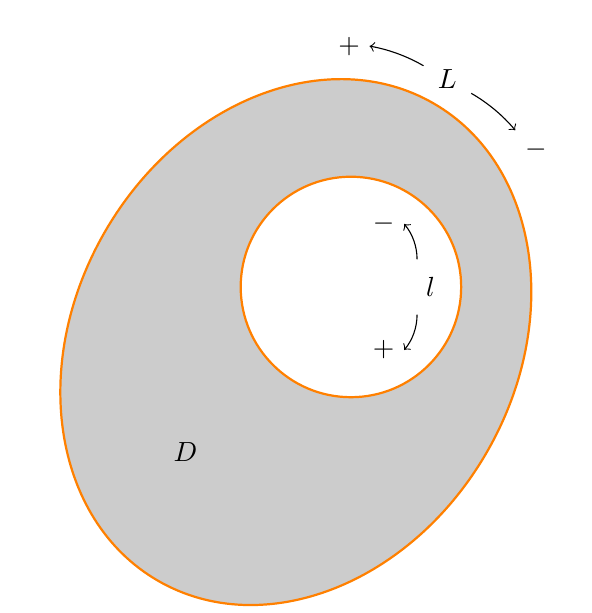
\begin{tikzpicture}[scale=.7]
	\draw[orange,fill=gray!40,rotate=60,thick] (0,0)ellipse[x radius=5,y radius=4];
	\draw[orange,fill=white,thick] (1,1)ellipse[x radius=2,y radius=2];
	\draw (-2,-2)node{\(D\)};
	\begin{scope}[rotate=60]
		\coordinate (P1) at (5.5,0);
		\draw (P1)node{\(L\)};
		\draw[->] (P1)+(0,.5) arc[start angle=0,end angle=20,radius=3]node[left]{\(+\)};
		\draw[->] (P1)+(0,-.5) arc[start angle=0,end angle=-20,radius=3]node[below right]{\(-\)};
	\end{scope}
	\begin{scope}
		\coordinate (P2) at (2.7,1);
		\draw (P2)node[left]{\(l\)};
		\draw[->] (P2)+(-.5,.5) arc[start angle=0,end angle=40,radius=1]node[left]{\(-\)};
		\draw[->] (P2)+(-.5,-.5) arc[start angle=0,end angle=-40,radius=1]node[left]{\(+\)};
	\end{scope}
\end{tikzpicture}
\caption{}
\label{figure:线积分与面积分.平面区域的边界曲线与其取向}
\end{figure}

\begin{theorem}[格林公式]
设闭区域\(D\)由分段光滑的曲线\(L\)围成,
函数\(P(x,y)\)和\(Q(x,y)\)在\(D\)上具有一阶连续偏导数,
则有
\begin{equation}\label{equation:线积分与面积分.格林公式}
	\iint_D \left( \pdv{Q}{x} - \pdv{P}{y} \right) \dd{x}\dd{y}
	= \oint_L P\dd{x} + Q\dd{y},
\end{equation}
其中\(L\)是\(D\)的取正向的边界曲线\footnote{%
如果\(D\)是复连通区域,
那么\cref{equation:线积分与面积分.格林公式}
右端应包括沿区域\(D\)的全部边界的曲线积分
(如\cref{figure:线积分与面积分.平面区域的边界曲线与其取向} 中的曲线\(L\)和\(l\)),
且边界的方向对区域\(D\)来说都是正向.}.
\end{theorem}
\cref{equation:线积分与面积分.格林公式} 叫做\DefineConcept{格林公式}.

为了方便记忆,我们可以利用行列式记号,把格林公式写成如下形式:\[
	\iint_D \begin{vmatrix}
		\pdv{x} & \pdv{y} \\
		P & Q
	\end{vmatrix} \dd{x}\dd{y}
	= \oint_L P\dd{x}+Q\dd{y}.
\]

下面说明格林公式的一个简单应用.
在格林公式中,
令\(P=-y\)、\(Q=x\),
可得\[
	2 \iint_D \dd{x}\dd{y}
	=\oint_L x\dd{y}-y\dd{x}.
\]
上式左端是闭区域\(D\)的面积\(A\)的两倍,
因此有
\begin{equation}\label{equation:线积分与面积分.利用格林公式计算闭区域的面积}
	A = \frac{1}{2} \oint_L x\dd{y}-y\dd{x}.
\end{equation}

\begin{example}
求椭圆\(x = a \cos\theta, y = b \sin\theta\)所围成图形的面积\(A\).
\begin{solution}
根据\cref{equation:线积分与面积分.利用格林公式计算闭区域的面积} 有
\begin{align*}
	A &= \frac{1}{2} \oint_L x\dd{y}-y\dd{x} \\
	&= \frac{1}{2} \int_0^{2\pi}
		\left[
			a \cos\theta \cdot b \cos\theta
			- b \sin\theta \cdot (-a \sin\theta)
		\right] \dd{\theta} \\
	&= \frac{1}{2} ab \int_0^{2\pi} \dd{\theta}
	= \pi ab.
\end{align*}
\end{solution}
\end{example}

\begin{example}
计算\(\oint_L \frac{x\dd{y}-y\dd{x}}{x^2+y^2}\),
其中\(L\)是一条不经过原点的分段光滑的若尔当闭曲线,
\(L\)的方向为逆时针方向.
\begin{solution}
记\(P = -\frac{y}{x^2+y^2}, Q = \frac{x}{x^2+y^2}\).
当\(x^2+y^2\neq0\)时,
有\[
	\pdv{Q}{x} = \frac{y^2-x^2}{(x^2+y^2)^2} = \pdv{P}{y}.
\]
记\(L\)所围成的闭区域为\(D\).

当\((0,0) \notin D\)时,
由\cref{equation:线积分与面积分.格林公式} 有\[
	\oint_L \frac{x\dd{y}-y\dd{x}}{x^2+y^2} = \iint_D 0 \dd{x}\dd{y} = 0;
\]

当\((0,0) \in D\)时,
取\(r>0\)使得\(D_r = \Set{ (x,y) \given x^2+y^2 < r^2 } \subseteq D\),
令\(l = \partial D_r\),
\(D_1 = D - D_r\).
对复连通区域\(D_1\)应用格林公式,
得\[
	\oint_L \frac{x\dd{y}-y\dd{x}}{x^2+y^2} - \oint_l \frac{x\dd{y}-y\dd{x}}{x^2+y^2}
	= \iint_{D_1} 0 \dd{x}\dd{y} = 0,
\]
其中\(l\)的方向取逆时针方向.
于是\[
	\oint_L \frac{x\dd{y}-y\dd{x}}{x^2+y^2}
	= \oint_l \frac{x\dd{y}-y\dd{x}}{x^2+y^2}
	= \int_0^{2\pi} \frac{r^2 \cos^2\theta + r^2 \sin^2\theta}{r^2} \dd{\theta}
	= 2\pi.
\]
综上所述\[
	\oint_L \frac{x\dd{y}-y\dd{x}}{x^2+y^2}
	= \begin{cases}
		2\pi, & (0,0) \in D, \\
		0, & (0,0) \notin D.
	\end{cases}
\]
\end{solution}
\end{example}

\begin{example}[二维格林第一公式、二维格林第二公式]
设\(u(x,y)\)、\(v(x,y)\)在闭区域\(D\)上都具有二阶连续偏导数,
分段光滑的曲线\(L\)为\(D\)的正向边界曲线.
证明:\begin{gather}
	\iint_D v \laplacian{u} \dd{x}\dd{y}
	= - \iint_D (\grad u \cdot \grad v) \dd{x}\dd{y} + \oint_L v \pdv{u}{\vb{n}} \dd{s};
	\label{equation:线积分与面积分.二维格林第一公式} \\
	\iint_D (u \laplacian v - v \laplacian u) \dd{x}\dd{y}
	= \oint_L \left( u \pdv{v}{\vb{n}} - v \pdv{u}{\vb{n}} \right) \dd{s},
	\label{equation:线积分与面积分.二维格林第二公式}
\end{gather}
其中\(\pdv{u}{\vb{n}}\)、\(\pdv{v}{\vb{n}}\)
分别是\(u\)、\(v\)沿\(L\)的外法线向量\(\vb{n}\)的方向导数,
二维拉普拉斯算子\(\laplacian = \pdv[2]{x} + \pdv[2]{y}\).
\begin{proof}
因为方向导数\[
	\pdv{u}{\vb{n}}
	= \pdv{u}{x} \cos\alpha
	+ \pdv{u}{y} \cos\beta,
	\qquad
	\pdv{v}{\vb{n}}
	= \pdv{v}{x} \cos\alpha
	+ \pdv{v}{y} \cos\beta,
\]其中\(\cos\alpha\)、\(\cos\beta\)是\(L\)在点\((x,y)\)处的外法线向量的方向余弦,
那么\(L\)在该点处的正向单位切向量为\(\vb{\tau} = (-\cos\beta,\cos\alpha)\),
于是利用格林公式可得\begin{align*}
	\oint_L v \pdv{u}{\vb{n}} \dd{s}
	&= \oint_L v \left(
	\pdv{u}{x} \cos\alpha
	+ \pdv{u}{y} \cos\beta
	\right) \dd{s} \\
	&= \oint_L \left( - v \pdv{u}{y} \right) \dd{x}
		+ \left( v \pdv{u}{x} \right) \dd{y} \\
	&= \iint_D \left[
		\pdv{x} \left( v \pdv{u}{x} \right)
		- \pdv{y} \left( - v \pdv{u}{y} \right)
		\right] \dd{x}\dd{y} \\
	&= \iint_D \left(
		\pdv{v}{x} \pdv{u}{x}
		+ v \pdv[2]{u}{x}
		+ \pdv{v}{y} \pdv{u}{y}
		+ v \pdv[2]{u}{y}
		\right) \dd{x}\dd{y} \\
	&= \iint_D (\grad u \cdot \grad v) \dd{x}\dd{y}
		+ \iint_D v \laplacian{u} \dd{x}\dd{y},
\end{align*}
移项可得\[
	\iint_D v \laplacian{u} \dd{x}\dd{y}
	= - \iint_D (\grad u \cdot \grad v) \dd{x}\dd{y}
	+ \oint_L v \pdv{u}{\vb{n}} \dd{s}.
	\eqno(1)
\]
同理可得\[
	\iint_D u \laplacian{v} \dd{x}\dd{y}
	= - \iint_D (\grad v \cdot \grad u) \dd{x}\dd{y}
	+ \oint_L u \pdv{v}{\vb{n}} \dd{s}.
	\eqno(2)
\]
(2)式与(1)式相减便得\[
	\iint_D (u \laplacian{v} - v \laplacian{u}) \dd{x}\dd{y}
	= \oint_L \left(
		u \pdv{v}{\vb{n}} - v \pdv{u}{\vb{n}}
	\right) \dd{s}.
	\qedhere
\]
\end{proof}
\end{example}

\begin{example}
设函数\(f(x,y)\)在区域\(D=\Set{(x,y) \given x^2+y^2\leq1}\)上具有二阶连续偏导数,
且\(\laplacian{f}=e^{-(x^2+y^2)}\),
求二重积分\(I=\iint_D\left(x\pdv{f}{x}+y\pdv{f}{y}\right)\dd{x}\dd{y}\).
\begin{solution}
考虑区域\(D\)的形状,将积分\(I\)化为在极坐标系下的积分,
令\(x=\rho\cos\theta, y=\rho\sin\theta\):
\begin{align*}
	I &= \int_0^1 \rho\dd{\rho} \int_0^{2\pi}
		\left(\rho\cos\theta\pdv{f}{x}+\rho\sin\theta\pdv{f}{y}\right) \dd{\theta} \\
	&= \int_0^1 \rho\dd{\rho} \int_0^{2\pi}
		\left[\pdv{f}{x}\dd(\rho\sin\theta)-\pdv{f}{y}\dd(\rho\cos\theta)\right].
\end{align*}
考虑到\(\dd{x}=\dd(\rho\cos\theta),
\dd{y}=\dd(\rho\sin\theta)\),
所以\[
	I = \int_0^1 \rho\dd{\rho} \oint_{L_\rho} \pdv{f}{x}\dd{y}-\pdv{f}{y}\dd{x}.
\]
其中\(L_\rho: x^2+y^2=\rho^2\).
令\(D_\rho = \Set{ (x,y) \given x^2+y^2\leq\rho^2 }\),
应用\hyperref[equation:线积分与面积分.格林公式]{格林公式},
则有\begin{align*}
	\oint_{L_\rho} \pdv{f}{x}\dd{y}-\pdv{f}{y}\dd{x}
	&= \iint_{D_\rho} \laplacian{f} \dd{x}\dd{y} \\
	&= \iint_{D_\rho} e^{-(x^2+y^2)} \dd{x}\dd{y} \\
	&= \int_0^{2\pi} \dd{\theta} \int_0^\rho e^{-r^2} r\dd{r} \\
	&= \pi \left(1-e^{-\rho^2}\right).
\end{align*}
那么\[
	I = \int_0^1 \pi \left(1-e^{-\rho^2}\right) \rho\dd{\rho}
	=  \frac{\pi}{2e}.
\]
\end{solution}
\end{example}

\subsection{平面上曲线积分与路径无关的条件}
在物理学中(特别是在力学中)要研究所谓“势场”,
就是要研究场力所作的功与路径无关的情形.
在什么条件下场力所作的功与路径无关?
这个问题在数学上就是要研究曲线积分与路径无关的条件.
为了研究这个问题,先要明确什么叫做“曲线积分\(\int_L P\dd{x}+Q\dd{y}\)与路径无关”.
\begin{definition}
设\(G\)是一个区域,\(P(x,y)\)以及\(Q(x,y)\)在区域\(G\)内具有一阶连续偏导数.
如果对于\(G\)内任意指定的两个点\(A\)、\(B\)
以及\(G\)内从点\(A\)到点\(B\)的任意两条曲线\(L_1\)、\(L_2\),
等式\[
	\int_{L_1} P\dd{x}+Q\dd{y}
	=\int_{L_2} P\dd{x}+Q\dd{y}
\]恒成立,
就说“曲线积分\(\int_L P\dd{x}+Q\dd{y}\)在\(G\)内与路径无关”
或“沿\(G\)内任意闭曲线\(C\)的曲线积分\(\oint_C P\dd{x}+Q\dd{y}\)等于零”,
否则便说“曲线积分\(\int_L P\dd{x}+Q\dd{y}\)在\(G\)内与路径相关”.
\end{definition}

\begin{theorem}\label{theorem:线积分与面积分.平面上曲线积分与路径无关的充要条件}
设区域\(G\)是一个单连通区域,
函数\(P(x,y)\)、\(Q(x,y)\)在\(G\)内具有一阶连续偏导数,
那么曲线积分\(\int_L P\dd{x}+Q\dd{y}\)在\(G\)内
与路径无关(或沿\(G\)内任意闭曲线的曲线积分为零)的充要条件是:\[
	\pdv{P}{y}=\pdv{Q}{x}
\]在\(G\)内恒成立.
\end{theorem}

如果\cref{theorem:线积分与面积分.平面上曲线积分与路径无关的充要条件}
所要求的两个条件“区域\(G\)是单连通区域,
且函数\(P(x,y)\)和\(Q(x,y)\)在\(G\)内具有一阶连续偏导数”不能同时满足,
那么定理的结论不能保证成立.

例如当区域\(G\)中出现破坏函数\(P\)、\(Q\)
及\(Q'_x\)、\(P'_y\)连续性条件的\DefineConcept{奇点}时,
定理的结论就不能保证成立.

\subsection{二元函数的全微分求积}
\begin{theorem}\label{theorem:线积分与面积分.二元函数的全微分的存在条件}
设区域\(G\)是一个单连通区域.
函数\(P(x,y)\)、\(Q(x,y)\)在\(G\)内具有一阶连续偏导数.
则\(P(x,y)\dd{x}+Q(x,y)\dd{y}\)在\(G\)内为某一函数\(u(x,y)\)的全微分的充要条件是\[
\pdv{P}{y}=\pdv{Q}{x}
\]在\(G\)内恒成立.
\end{theorem}

根据\cref{theorem:线积分与面积分.平面上曲线积分与路径无关的充要条件,theorem:线积分与面积分.二元函数的全微分的存在条件},
立即可得如下推论.
\begin{corollary}
设区域\(G\)是一个单连通区域.
函数\(P(x,y)\)、\(Q(x,y)\)在\(G\)内具有一阶连续偏导数.
则曲线积分\(\int_L P\dd{x}+Q\dd{y}\)在\(G\)内与路径无关的充要条件是:
在\(G\)内存在函数\(u(x,y)\),使\(\dd{u}=P\dd{x}+Q\dd{y}\).
\end{corollary}

\subsection{曲线积分的基本定理}
\begin{definition}
若曲线积分\(\int_L \vb{F}\cdot\dd{\vb{r}}\)在区域\(G\)内与积分路径无关,
则称向量场\(\vb{F}\)为\DefineConcept{保守场}.
\end{definition}

下面的定理给出了平面曲线积分与路径无关的另一种形式的条件,
并为计算保守场中的曲线积分提供了一种简便的方法.
\begin{theorem}[曲线积分的基本定理]\label{theorem:线积分与面积分.曲线积分的基本定理}
设\(\vb{F}(x,y)=P(x,y)\vb{i}+Q(x,y)\vb{j}\)是平面区域\(G\)内的一个向量场,
\(P(x,y)\)、\(Q(x,y)\)都在\(G\)内连续,
且存在一个数量函数\(f(x,y)\),使得\(\vb{F}=\grad f\),
则曲线积分\(\int_L\vb{F}\cdot\dd{\vb{r}}\)在\(G\)内与路径无关,且
\begin{equation}\label{equation:线积分与面积分.曲线积分的基本公式}
	\int_L \vb{F} \cdot \dd{\vb{r}}
	= f(B)-f(A),
\end{equation}
其中\(L\)是位于\(G\)内起点为\(A\)、终点为\(B\)的任一分段光滑曲线.
\end{theorem}

\cref{theorem:线积分与面积分.曲线积分的基本定理} 表明,
对于势场\(\vb{F}\),
曲线积分\(\int_L \vb{F}\cdot\dd{\vb{r}}\)的值仅依赖于它的势函数\(f\)在路径\(L\)的两端点的值,
而不依赖于两点间的路径,
即积分\(\int_L \vb{F}\cdot\dd{\vb{r}}\)在\(G\)内与路径无关.
也就是说:势场是保守场.

\cref{equation:线积分与面积分.曲线积分的基本公式}
是与微积分基本公式\[
	\int_a^b f(x) \dd{x}
	= F(b) - F(a)
\]
(其中\(F'(x) = f(x)\))完全类似的向量微积分的相应公式,
称为\DefineConcept{曲线积分的基本公式}.

\section{对面积的曲面积分}
\subsection{对面积的曲面积分的概念}
\begin{definition}
设曲面\footnote{以后都假定曲面的边界曲线是分段光滑的闭曲线,且曲面有界.}%
\(\Sigma\)是光滑的\footnote{如果曲面上各点处都具有切平面,则称该曲面是光滑的.
如果曲面是由有限个光滑曲面所组成的,则称该曲面是分片光滑的.}.
函数\(f(x,y,z)\)在\(\Sigma\)上有界.
把\(\Sigma\)任意分成\(n\)小块\(\increment S_i\)
(\(\increment S_i\)同时也代表第\(i\)小块曲面的面积),
设\(\opair{\xi_i,\eta_i,\zeta_i}\)是\(\increment S_i\)上任取的一点,
作乘积\(f(\xi_i,\eta_i,\zeta_i) \increment S_i\ (i=1,2,\dotsc,n)\),
并作和\(\sum\limits_{i=1}^n f(\xi_i,\eta_i,\zeta_i) \increment S_i\),
如果当各小块曲面的直径\footnote{%
曲面的直径是指曲面上任意两点间距离的最大者.}的最大值\(\lambda\to0\)时,
这和的极限总存在,
则称此极限为
“函数\(f(x,y,z)\)在曲面\(\Sigma\)上\DefineConcept{对面积的曲面积分}”
或“函数\(f(x,y,z)\)在曲面\(\Sigma\)上的\DefineConcept{第一类曲面积分}%
(type I surface integral)”,
记作\(\iint_\Sigma{f(x,y,z)\dd{S}}\),
即\[
	\iint_\Sigma f(x,y,z)\dd{S}
	\defeq
	\lim\limits_{\lambda\to0} \sum\limits_{i=1}^n f(\xi_i,\eta_i,\zeta_i) \increment S_i,
\]
其中\(f(x,y,z)\)叫做\DefineConcept{被积函数},
\(\Sigma\)叫做\DefineConcept{积分曲面}.

如果曲面\(\Sigma\)是分片光滑的,
我们规定:
函数在\(\Sigma\)上对面积的曲面积分,
等于函数在光滑的各片曲面上对面积的曲面积分之和.
\end{definition}
我们指出,当被积函数\(f(x,y,z)\)在光滑曲面\(\Sigma\)上连续时,对面积的曲面积分是存在的.

\subsection{对面积的曲面积分的性质}
由对面积的曲面积分的定义可知,它具有与对弧长的曲线积分相类似的性质,这里不再赘述.

\subsection{对面积的曲面积分的计算法}
\begin{theorem}
设积分曲面\(\Sigma\)由方程\(z=z(x,y)\)给出,
\(\Sigma\)在\(xOy\)面上的投影区域为\(D_{xy}\),
函数\(z=z(x,y)\)在\(D_{xy}\)上具有连续偏导数,
被积函数\(f(x,y,z)\)在\(\Sigma\)上连续.
那么有\[
\iint_\Sigma{f(x,y,z)\dd{S}}
=\iint_{D_{xy}}{f[x,y,z(x,y)] \sqrt{1+[z'_x(x,y)]^2+[z'_y(x,y)]^2} \dd{x}\dd{y}}.
\]
\end{theorem}
这就是把对面积的曲面积分化为二重积分的公式.
在计算时,只要把变量\(z\)换为\(z(x,y)\),\(\dd{S}\)换为
\(\sqrt{1+(z'_x)^2+(z'_y)^2} \dd{x}\dd{y}\),
再确定\(\Sigma\)在\(xOy\)面上的投影区域\(D_{xy}\),
这样就把对面积的曲面积分化为二重积分了.

如果积分曲面\(\Sigma\)由方程\(x=x(y,z)\)或\(y=y(z,x)\)给出,
也可类似地把对面积的曲面积分化为相应的二重积分.

可以将上述对面积的曲面积分的计算法总结为如下更一般的方法.
\begin{theorem}
设积分曲面\(\Sigma\)由二元向量值参数方程\[
	\mat{r}(u,v) = x(u,v) \mat{i} + y(u,v) \mat{j} + z(u,v) \mat{k},
	\quad \opair{u,v} \in D
\]给出,
函数\(\mat{r}(u,v)\)在\(D\)上具有连续偏导数,
被积函数\(f(x,y,z)\)在\(\Sigma\)上连续,
那么有\[
	\iint_\Sigma f(x,y,z) \dd{S}
	= \iint_D f[\mat{r}(u,v)]
	\abs{\mat{r}'_u \times \mat{r}'_v}
	\dd{\sigma}.
\]
\end{theorem}
这里,参数\(u\)、\(v\)可以代换为\(x\)、\(y\)、\(z\)中任意两个,
区域\(D\)可以代换为\(D_{xy}\)、\(D_{yz}\)或\(D_{zx}\).

\begin{example}
计算曲面积分\(\iint_\Sigma \frac{\dd{S}}{z}\),
其中\(\Sigma\)是球面\(x^2+y^2+z^2=a^2\)被平面\(z = h\ (0<h<a)\)截出的顶部.
\begin{solution}
\(\Sigma\)的方程为\(z = \sqrt{a^2-x^2-y^2}\).
\(\Sigma\)在\(xOy\)面上的投影区域\(D_{xy}\)为圆形闭区域\[
	\Set{\opair{x,y} \given x^2+y^2 \leq a^2-h^2}.
\]
又\[
	\sqrt{1+(z'_x)^2+(z'_y)^2} = \frac{a}{\sqrt{a^2-x^2-y^2}},
\]
所以\[
	\iint_\Sigma \frac{\dd{S}}{z}
	= \iint_{D_{xy}} \frac{a\dd{x}\dd{y}}{a^2-x^2-y^2}.
\]
利用极坐标,得\[
	\iint_\Sigma \frac{\dd{S}}{z}
	= \iint_{D_{xy}} \frac{a\rho\dd{\rho}\dd{\theta}}{a^2-\rho^2}
	= a \int_0^{2\pi} \dd{\theta} \int_0^{\sqrt{a^2-h^2}} \frac{\rho\dd{\rho}}{a^2-\rho^2}
	= 2\pi a \ln\frac{a}{h}.
\]
\end{solution}
\end{example}

\begin{example}
计算\(\varoiint_\Sigma xyz \dd{S}\),
其中\(\Sigma\)是由平面\(x=0\)、\(y=0\)、\(z=0\)及\(x+y+z=1\)所围成的四面体的整个边界曲面.
\begin{solution}
整个边界曲面\(\Sigma\)在平面\(x=0\)、\(y=0\)、\(z=0\)及\(x+y+z=1\)上的部分
依次记为\(\AutoTuple{\Sigma}{4}\),于是\[
	\varoiint_\Sigma xyz \dd{S}
	= \varoiint_{\Sigma_1} xyz \dd{S}
	+ \varoiint_{\Sigma_2} xyz \dd{S}
	+ \varoiint_{\Sigma_3} xyz \dd{S}
	+ \varoiint_{\Sigma_4} xyz \dd{S}.
\]
由于在\(\AutoTuple{\Sigma}{3}\)上,被积函数\(f(x,y,z)=xyz\)均为零,所以\[
	\varoiint_{\Sigma_1} xyz \dd{S}
	= \varoiint_{\Sigma_2} xyz \dd{S}
	= \varoiint_{\Sigma_3} xyz \dd{S}
	= 0.
\]

在\(\Sigma_4\)上,\(z=1-x-y\),\(z'_x = z'_y = -1\),所以\[
	\sqrt{1+(z'_x)^2+(z'_y)^2}
	= \sqrt{1+(-1)^2+(-1)^2}
	= \sqrt{3},
\]
从而\[
	\varoiint_\Sigma xyz \dd{S}
	= \varoiint_{\Sigma_4} xyz \dd{S}
	= \iint_{D_{xy}} \sqrt{3} xy (1-x-y) \dd{x} \dd{y},
\]
其中\(D_{xy}\)是\(\Sigma_4\)在\(xOy\)面上的投影区域,
即由直线\(x=0\)、\(y=0\)及\(x+y=1\)所围成的闭区域.
因此\[
	\varoiint_\Sigma xyz \dd{S}
	= \sqrt{3} \int_0^1 x \dd{x} \int_0^{1-x} y (1-x-y) \dd{y}
	= \frac{\sqrt{3}}{120}.
\]
\end{solution}
\end{example}

\begin{example}
设点\(P\)是椭球面\(S: x^2 + y^2 + z^2 - yz = 1\)上的动点,
若\(S\)在点\(P\)处的切平面与\(xOy\)面垂直,求点\(P\)的轨迹\(C\),并计算曲面积分\[
	I = \iint_\Sigma \frac{(x+\sqrt{3}) \abs{y-2z}}{\sqrt{4+y^2+z^2-4yz}} \dd{S},
\]
其中\(\Sigma\)是椭球面\(S\)位于曲线\(C\)上方的部分.
\begin{solution}
设\(F(x,y,z) = x^2 + y^2 + z^2 - yz - 1\).
求导得\[
	F'_x = 2x, \qquad
	F'_y = 2y - z, \qquad
	F'_z = 2z - y,
\]
那么\(S\)在点\(P(x,y,z)\)处的切向量为\(\mat{n} = \opair{2x,2y-z,2z-y}\).
因为点\(P\)处的切平面与\(xOy\)面垂直,
所以法向量\(\mat{n}\)与\(xOy\)面的法向量\(\opair{0,0,1}\)垂直,\[
	2x\cdot0 + (2y-z)\cdot0+(2z-y)\cdot1=0
	\quad\text{或}\quad
	2z-y=0.
\]
因此,轨迹\(C\)的方程是\[
	\begin{cases}
		x^2 + y^2 + z^2 - yz = 1, \\
		2z-y=0.
	\end{cases}
\]
消去轨迹\(C\)方程中的\(z\),得到\(C\)在\(xOy\)面上的投影为\[
	C_{xy}: x^2+\frac{3}{4}y^2=1.
\]
又因为\[
	z'_x = - \frac{F'_x}{F'_z} = \frac{2x}{y-2z}, \qquad
	z'_y = - \frac{F'_y}{F'_z} = \frac{2y-z}{y-2z},
\]
\begin{align*}
	\dd{S} &= \sqrt{1+(z'_x)^2+(z'_y)^2} \dd{x}\dd{y} \\
	&= \sqrt{1+\left(\frac{2x}{y-2z}\right)^2+\left(\frac{2y-z}{y-2z}\right)^2} \dd{x}\dd{y} \\
	&= \frac{\sqrt{4x^2+5y^2+5z^2-8yz}}{\abs{y-2z}} \dd{x}\dd{y} \\
	&= \frac{\sqrt{4+y^2+z^2-4yz}}{\abs{y-2z}} \dd{x}\dd{y},
\end{align*}
所以\begin{align*}
	&\hspace{-20pt}
	\iint_\Sigma \frac{(x+\sqrt{3}) \abs{y-2z}}{\sqrt{4+y^2+z^2-4yz}} \dd{S} \\
	&= \iint_{x^2+\frac{3}{4}y^2\leq1} \frac{(x+\sqrt{3}) \abs{y-2z}}{\sqrt{4+y^2+z^2-4yz}}
		\cdot \frac{\sqrt{4+y^2+z^2-4yz}}{\abs{y-2z}} \dd{x}\dd{y} \\
	&= \iint_{x^2+\frac{3}{4}y^2\leq1} (x+\sqrt{3}) \dd{x}\dd{y} \\
	&= \sqrt{3} \iint_{x^2+\frac{3}{4}y^2\leq1} \dd{x}\dd{y}
	= 2\pi.
\end{align*}
\end{solution}
\end{example}

\subsection{利用对称性简化第一类曲面积分的计算}
设积分曲面\(\Sigma\)关于\(xOy\)面对称.
若被积函数\(f(x,y,z)\)是关于\(z\)的偶函数,
即\(f(x,y,-z) = f(x,y,z)\),则\[
	\iint_\Sigma f(x,y,z) \dd{S}
	= 2 \iint_{D_{xy}} f[x,y,z(x,y)] \sqrt{1+(z'_x)^2+(z'_y)^2} \dd{x}\dd{y};
\]
若被积函数\(f(x,y,z)\)是关于\(z\)的奇函数,
即\(f(x,y,-z) = -f(x,y,z)\),则\[
	\iint_\Sigma f(x,y,z) \dd{S} = 0.
\]

类似地,可以得出,在积分曲面关于\(yOz\)面或\(zOx\)面对称,
而被积函数\(f(x,y,z)\)是关于\(x\)或\(y\)的奇函数或偶函数的情形下,
第一类曲面积分的简化计算公式.

\begin{example}
计算\(\varoiint_\Sigma x^2 \dd{S}\),其中\(\Sigma: x^2+y^2+z^2=a^2\).
\begin{solution}
利用对称性可得\begin{align*}
	\varoiint_\Sigma x^2 \dd{S}
	&= \frac{1}{3} \varoiint_\Sigma (x^2+y^2+z^2) \dd{S} \\
	&= \frac{1}{3} \varoiint_\Sigma a^2 \dd{S}
	= \frac{a^2}{3} \varoiint_\Sigma \dd{S} \\
	&= \frac{a^2}{3} \cdot 4\pi a^2
	= \frac{4}{3} \pi a^4.
\end{align*}
\end{solution}
\end{example}

\section{对坐标的曲面积分}
\subsection{对坐标的曲面积分的概念}
通常我们遇到的曲面都是双侧的.
例如由方程\(z = z(x,y)\)表示的曲面,
有上侧与下侧之分\footnote{按惯例,这里假定\(z\)轴竖直向上.};
又例如,一张包围某一空间区域的闭曲面,有外侧与内侧之分.
以后我们总假定所考虑的曲面是双侧的.

在讨论对坐标的曲面积分时,需要制定曲面的侧.
我们可以通过曲面上的法向量的指向来定出曲面的侧.
例如,对于曲面\(z = z(x,y)\),如果取它的法向量\(\vb{n}\)的指向朝上,我们就认为取定曲面的上侧;
又如,对于闭曲面如果取它的法向量的指向朝外,我们就认为取定曲面的外侧.
这种取定了法向量亦即选定了侧的曲面,就称为\DefineConcept{有向曲面}.

设\(\Sigma\)是有向曲面.
在\(\Sigma\)上取一小块曲面\(\increment S\),
把\(\increment S\)投影到\(xOy\)面上得一投影区域,
这投影区域的面积记为\((\increment\sigma)_{xy}\).
假定\(\increment S\)上各点处的法向量
与\(z\)轴的夹角\(\gamma\)的余弦\(\cos\gamma\)有相同的符号
(即\(\cos\gamma\)都是正的或都是负的).
我们规定\(\increment S\)在\(xOy\)面上的投影\((\increment S)_{xy}\)为\[
	(\increment S)_{xy}
	= \sgn\cos\gamma \cdot (\increment \sigma)_{xy}
	= \left\{ \begin{array}{cc}
	(\increment \sigma)_{xy}, & \cos\gamma > 0, \\
	-(\increment \sigma)_{xy}, & \cos\gamma < 0, \\
	0, & \cos\gamma \equiv 0.
	\end{array} \right.
\]
其中,\(\cos\gamma \equiv 0\)也就是\((\increment \sigma)_{xy} = 0\)的情形.
\(\increment S\)在\(xOy\)面上的投影\((\increment S)_{xy}\)
实际就是\(\increment S\)在\(xOy\)面上的投影区域的面积附以一定的正负号.
类似地可以定义\(\increment S\)在\(yOz\)面及\(zOx\)面上的
投影\((\increment S)_{yz}\)和\((\increment S)_{zx}\).

设\(\Sigma\)为光滑的有向曲面,函数\(R(x,y,z)\)在\(\Sigma\)上有界.
把\(\Sigma\)任意分成\(n\)块小曲面\(\increment S_i\)%
(\(\increment S_i\)同时又表示第\(i\)块小曲面的面积),
\(\increment S_i\)在\(xOy\)面上的投影为\((\increment S_i)_{xy}\),
\((\xi_i,\eta_i,\zeta_i)\)是\(\increment S_i\)上任意取定的一点.
如果当各小块曲面的直径的最大值\(\lambda\to0\)时,极限\[
	\lim\limits_{\lambda\to0}
	\sum\limits_{i=1}^n
	R(\xi_i,\eta_i,\zeta_i)
	(\increment S_i)_{xy}
\]总存在,
则称此极限为
“函数\(R(x,y,z)\)在有向曲面\(\Sigma\)上对坐标\(x\)、\(y\)的\DefineConcept{曲面积分}”,
记作\[
	\iint_\Sigma R(x,y,z) \dd{x}\dd{y},
\]
即\[
	\iint_\Sigma R(x,y,z) \dd{x}\dd{y}
	\defeq
	\lim\limits_{\lambda\to0}
	\sum\limits_{i=1}^n
	R(\xi_i,\eta_i,\zeta_i)
	(\increment S_i)_{xy},
\]
其中\(R(x,y,z)\)叫做\DefineConcept{被积函数},\(\Sigma\)叫做\DefineConcept{积分曲面}.

类似地可以定义
“函数\(P(x,y,z)\)在有向曲面\(\Sigma\)上对坐标\(y\)、\(z\)的\DefineConcept{曲面积分}”
及“函数\(Q(x,y,z)\)在有向曲面\(\Sigma\)上对坐标\(z\)、\(x\)的\DefineConcept{曲面积分}”
分别为\begin{gather*}
	\iint_\Sigma P(x,y,z) \dd{y}\dd{z}
	\defeq
	\lim\limits_{\lambda\to0}
	\sum\limits_{i=1}^n P(\xi_i,\eta_i,\zeta_i) (\increment S_i)_{yz}, \\
	\iint_\Sigma Q(x,y,z) \dd{z}\dd{x}
	\defeq
	\lim\limits_{\lambda\to0}
	\sum\limits_{i=1}^n Q(\xi_i,\eta_i,\zeta_i) (\increment S_i)_{zx}.
\end{gather*}

以上三个曲面积分也称为\DefineConcept{第二类曲面积分}(type II surface integral).

如果\(\Sigma\)是分片光滑的有向曲面,我们规定函数在\(\Sigma\)上对坐标的曲面积分等于函数在各片光滑曲面上对坐标的曲面积分之和.

我们指出,当\(P(x,y,z),Q(x,y,z),R(x,y,z)\)在有向光滑曲面\(\Sigma\)上连续时,对坐标的曲面积分是存在的.

一般地,可以将\[
\iint_\Sigma P(x,y,z) \dd{y}\dd{z}
+\iint_\Sigma Q(x,y,z) \dd{z}\dd{x}
+\iint_\Sigma R(x,y,z) \dd{x}\dd{y}
\]合并写成\[
\iint_\Sigma{P(x,y,z)\dd{y}\dd{z}+Q(x,y,z)\dd{z}\dd{x}+R(x,y,z)\dd{x}\dd{y}}.
\]

\subsection{对坐标的曲面积分的性质}
对坐标的曲面积分具有与对坐标的曲线积分相类似的一些性质.
\begin{property}
如果把\(\Sigma\)分成\(\Sigma_1\)和\(\Sigma_2\),则\begin{align*}
&\iint_\Sigma{P\dd{y}\dd{z}+Q\dd{z}\dd{x}+R\dd{x}\dd{y}} \\
&\qquad=\iint_{\Sigma_1}{P\dd{y}\dd{z}+Q\dd{z}\dd{x}+R\dd{x}\dd{y}} \\
&\qquad\quad+\iint_{\Sigma_2}{P\dd{y}\dd{z}+Q\dd{z}\dd{x}+R\dd{x}\dd{y}}.
\end{align*}
\end{property}

\begin{property}
设\(\Sigma\)是有向曲面,\(\Sigma^-\)表示与\(\Sigma\)取相反侧的有向曲面,则\begin{gather*}
\iint_{\Sigma^-} P(x,y,z) \dd{y}\dd{z} = -\iint_\Sigma P(x,y,z) \dd{y}\dd{z}, \\
\iint_{\Sigma^-} Q(x,y,z) \dd{z}\dd{x} = -\iint_\Sigma Q(x,y,z) \dd{z}\dd{x}, \\
\iint_{\Sigma^-} R(x,y,z) \dd{x}\dd{y} = -\iint_\Sigma R(x,y,z) \dd{x}\dd{y}.
\end{gather*}
\end{property}

\subsection{对坐标的曲面积分的计算法}
\begin{theorem}
设被积函数\(P(x,y,z)\)、\(Q(x,y,z)\)和\(R(x,y,z)\)在\(\Sigma\)上连续.
又设积分曲面\(\Sigma\)的单位法向量为\(\vb{n} = (\cos\alpha,\cos\beta,\cos\gamma)\).

如果\(\Sigma\)由\(z=z(x,y)\)给出,
且\(z=z(x,y)\)在\(D_{xy}\)上具有一阶连续偏导数,
则有\begin{equation}\label{equation:线积分与面积分.第二类曲面积分的计算式1}
	\iint_\Sigma R(x,y,z) \dd{x}\dd{y}
	= \sgn\cos\gamma \cdot \iint_{D_{xy}} R[x,y,z(x,y)] \dd{x}\dd{y}.
\end{equation}
\(\sgn\cos\gamma\)的取值可以这样判定:
当积分曲面为\(\Sigma\)上侧时,上式等号右侧取正号;
当积分曲面为\(\Sigma\)下侧时,上式等号右侧取负号.

如果\(\Sigma\)由\(y=y(z,x)\)给出,
且\(y=y(z,x)\)在\(D_{zx}\)上具有一阶连续偏导数,
则有\begin{equation}\label{equation:线积分与面积分.第二类曲面积分的计算式2}
	\iint_\Sigma Q(x,y,z) \dd{z}\dd{x}
	= \sgn\cos\beta \cdot \iint_{D_{zx}} Q[x,y(z,x),z] \dd{z}\dd{x}.
\end{equation}
\(\sgn\cos\beta\)的取值可以这样判定:
当积分曲面为\(\Sigma\)右侧时,上式等号右侧取正号;
当积分曲面为\(\Sigma\)左侧时,上式等号右侧取负号.

如果\(\Sigma\)由\(x=x(y,z)\)给出,
且\(x=x(y,z)\)在\(D_{yz}\)上具有一阶连续偏导数,
则有\begin{equation}\label{equation:线积分与面积分.第二类曲面积分的计算式3}
	\iint_\Sigma P(x,y,z) \dd{y}\dd{z}
	= \sgn\cos\alpha \cdot \iint_{D_{yz}} P[x(y,z),y,z] \dd{y}\dd{z}.
\end{equation}
\(\sgn\cos\alpha\)的取值可以这样判定:
当积分曲面为\(\Sigma\)前侧时,上式等号右侧取正号;
当积分曲面为\(\Sigma\)后侧时,上式等号右侧取负号.
\end{theorem}

可以将上述对坐标的曲面积分的计算法总结为如下更一般的方法.
\begin{theorem}
设积分曲面\(\Sigma\)由二元向量值参数方程\[
	\vb{r}(u,v) = x(u,v) \vb{i} + y(u,v) \vb{j} + z(u,v) \vb{k},
	\quad (u,v) \in D
\]给出,
这里\(D\)是\(uv\)平面上具有分段光滑边界的有界闭区域,
且\(\vb{r}\colon D \to \Sigma\)是具有一阶连续偏导数的单值函数,
且雅克比矩阵\[
	\vb{J} = \begin{bmatrix}
		x'_u & x'_v \\
		y'_u & y'_v \\
		z'_u & z'_v
	\end{bmatrix}
\]是满秩的,
且被积函数\[
	\vb{F}(x,y,z) = P(x,y,z) \vb{i} + Q(x,y,z) \vb{j} + R(x,y,z) \vb{k}
\]在\(\Sigma\)上连续,
那么有\begin{equation}
	\iint_\Sigma \vb{F} \cdot \dd{\vb{S}}
	= \iint_D \vb{F}(\vb{r}(u,v)) \cdot (\vb{r}'_u \times \vb{r}'_v) \dd{\sigma}.
\end{equation}
\end{theorem}

\begin{example}
计算曲面积分\[
	\iint_\Sigma x^2 \dd{y}\dd{z} + y^2 \dd{z}\dd{x} + z^2 \dd{x}\dd{y},
\]
其中\(\Sigma\)是长方体\(\Omega = \Set{
	(x,y,z)
	\given
	0 \leq x \leq a,
	0 \leq y \leq b,
	0 \leq z \leq c
}\)的整个表面的外侧.
\begin{solution}
把有向曲面\(\Sigma\)分成以下六部分:
\begin{center}
	\begin{tabular}{l}
		\(\Sigma_1: z=c\ (0 \leq x \leq a, 0 \leq y \leq b)\)的上侧; \\
		\(\Sigma_2: z=0\ (0 \leq x \leq a, 0 \leq y \leq b)\)的下侧; \\
		\(\Sigma_3: x=a\ (0 \leq y \leq b, 0 \leq z \leq c)\)的前侧; \\
		\(\Sigma_4: x=0\ (0 \leq y \leq b, 0 \leq z \leq c)\)的后侧; \\
		\(\Sigma_5: y=b\ (0 \leq x \leq a, 0 \leq z \leq c)\)的右侧; \\
		\(\Sigma_6: y=0\ (0 \leq x \leq a, 0 \leq z \leq c)\)的左侧. \\
	\end{tabular}
\end{center}
除\(\Sigma_3\)、\(\Sigma_4\)外,
其余四片曲面在\(yOz\)面上的投影为零,
因此\[
	\iint_\Sigma x^2 \dd{y}\dd{z}
	= \iint_{\Sigma_3} x^2 \dd{y}\dd{z}
	+ \iint_{\Sigma_4} x^2 \dd{y}\dd{z}.
\]
应用\cref{equation:线积分与面积分.第二类曲面积分的计算式3} 就有\[
	\iint_\Sigma x^2 \dd{y}\dd{z}
	= \iint_{D_{yz}} a^2 \dd{y}\dd{z}
	- \iint_{D_{yz}} 0^2 \dd{y}\dd{z}
	= a^2 bc.
\]
同理可得\[
	\iint_\Sigma y^2 \dd{z}\dd{x}
	= b^2 ac,
\]\[
	\iint_\Sigma z^2 \dd{x}\dd{y}
	= c^2 ab.
\]
于是所求曲面积分为\((a+b+c) abc\).
\end{solution}
\end{example}

\begin{example}
计算曲面积分\(\iint_\Sigma xyz \dd{x}\dd{y}\),
其中\(\Sigma\)是球面\(x^2+y^2+z^2=1\)外侧在\(x\geq0,y\geq0\)的部分.
\begin{solution}
把\(\Sigma\)分为\(\Sigma_1\)和\(\Sigma_2\)两部分,
其中\(\Sigma_1\)的方程为\[
	z = -\sqrt{1-x^2-y^2},
\]
而\(\Sigma_2\)的方程为\[
	z = \sqrt{1-x^2-y^2}.
\]
因此\begin{align*}
	\iint_\Sigma xyz \dd{x}\dd{y}
	&= \iint_{\Sigma_1} xyz \dd{x}\dd{y}
	+ \iint_{\Sigma_2} xyz \dd{x}\dd{y} \\
	&= -\iint_{D_{xy}} xy (-\sqrt{1-x^2-y^2}) \dd{x}\dd{y}
	+ \iint_{D_{xy}} xy \sqrt{1-x^2-y^2} \dd{x}\dd{y} \\
	&= 2 \iint_{D_{xy}} xy \sqrt{1-x^2-y^2} \dd{x}\dd{y}.
\end{align*}
其中\(D_{xy}\)是\(\Sigma_1,\Sigma_2\)在\(xOy\)面上的投影区域,
就是位于第一象限内的扇形\[
	x^2+y^2\leq1 \quad(x\geq0,y\geq0).
\]
利用极坐标计算这个二重积分如下:\[
	\iint_{D_{xy}} xy \sqrt{1-x^2-y^2} \dd{x}\dd{y}
	= \int_0^{\frac\pi2} \sin\theta \cos\theta \dd{\theta}
		\int_0^1 \rho^3 \sqrt{1-\rho^2} \dd{\rho}
	= \frac{1}{15},
\]
从而\(\iint_\Sigma xyz \dd{x}\dd{y} = \frac{2}{15}\).
\end{solution}
\end{example}

\subsection{利用对称性简化第二类曲面积分的计算}
设积分曲面\(\Sigma\)关于\(xOy\)面对称.
\begin{enumerate}
	\item 若被积函数\(f(x,y,z)\)是关于\(z\)的偶函数,即\[
		f(x,y,-z) = f(x,y,z),
	\]
	则\[
		\iint_\Sigma f(x,y,z) \dd{x}\dd{y} = 0;
	\]

	\item 若被积函数\(f(x,y,z)\)是关于\(z\)的奇函数,即\[
		f(x,y,-z) = -f(x,y,z),
	\]
	则\[
		\iint_\Sigma f(x,y,z) \dd{x}\dd{y}
		= 2 \sgn\cos\gamma \cdot \iint_{D_{xy}} f[x,y,z(x,y)] \dd{x}\dd{y}.
	\]
\end{enumerate}

类似地,可以得出,在积分曲面关于\(yOz\)面或\(zOx\)面对称,
而被积函数\(f(x,y,z)\)是关于\(x\)或\(y\)的奇函数或偶函数的情形下,
第二类曲面积分的简化计算公式.

\section{两类曲面积分之间的联系}
设有向曲面\(\Sigma\)由方程\(z = z(x,y)\)给出,
\(\Sigma\)在\(xOy\)面上的投影区域为\(D_{xy}\),
函数\(z = z(x,y)\)在\(D_{xy}\)上具有一阶连续偏导数,
\(R(x,y,z)\)在\(\Sigma\)上连续.
如果\(\Sigma\)取上侧,
则由对坐标的曲面积分计算公式 \labelcref{equation:线积分与面积分.第二类曲面积分的计算式1} 有\[
	\iint_\Sigma R(x,y,z) \dd{x}\dd{y} = \iint_{D_{xy}} R[x,y,z(x,y)] \dd{x}\dd{y}.
\]

另一方面,因上述有向曲面\(\Sigma\)的法向量的方向余弦为\[
	\begin{split}
		\cos\alpha=\frac{-z'_x}{\sqrt{1+(z'_x)^2+(z'_y)^2}}, \\
		\cos\beta=\frac{-z'_y}{\sqrt{1+(z'_x)^2+(z'_y)^2}}, \\
		\cos\gamma=\frac{1}{\sqrt{1+(z'_x)^2+(z'_y)^2}},
	\end{split}
\]
故由对面积的曲面积分计算公式 \labelcref{equation:线积分与面积分.第一类曲面积分的计算式1} 有\[
	\iint_\Sigma R(x,y,z) \cos\gamma \dd{S}
	= \iint_{D_{xy}} R[x,y,z(x,y)] \dd{x}\dd{y}.
\]
由此可见,有\begin{equation}\label{equation:两类曲面积分之间的联系.关系式1}
	\iint_\Sigma R(x,y,z) \dd{x}\dd{y}
	= \iint_\Sigma R(x,y,z) \cos\gamma \dd{S}.
\end{equation}
注意到等号两边的积分曲面都是\(\Sigma\),
被积函数都是\(R(x,y,z)\),
于是在形式上有\(\dd{x}\dd{y} = \cos\gamma \dd{S}\).

如果\(\Sigma\)取下侧,则\[
	\iint_\Sigma R(x,y,z) \cos\gamma \dd{S}
	= -\iint_{D_{xy}} R[x,y,z(x,y)] \dd{x}\dd{y}.
\]
但这时\(\cos\gamma=\frac{-1}{\sqrt{1+(z'_x)^2+(z'_y)^2}}\),
因此\cref{equation:两类曲面积分之间的联系.关系式1} 仍成立.

类似地可推得\begin{gather}
	\iint_\Sigma P(x,y,z) \dd{y}\dd{z}
	= \iint_{D_{yz}} P(x,y,z) \cos\alpha \dd{S},
	\label{equation:两类曲面积分之间的联系.关系式2} \\
	\iint_\Sigma Q(x,y,z) \dd{z}\dd{x}
	= \iint_{D_{zx}} Q(x,y,z) \cos\beta \dd{S}.
	\label{equation:两类曲面积分之间的联系.关系式3}
\end{gather}

合并\cref{equation:两类曲面积分之间的联系.关系式1,equation:两类曲面积分之间的联系.关系式2,equation:两类曲面积分之间的联系.关系式3},
得两类曲面积分之间的如下联系:
\begin{equation}\label{equation:线积分与面积分.两类曲面积分之间的联系}
	\iint_\Sigma P \dd{y}\dd{z} + Q \dd{z}\dd{x} + R \dd{x}\dd{y}
	=\iint_\Sigma (P\cos\alpha+Q\cos\beta+R\cos\gamma) \dd{S},
\end{equation}
其中\(\cos\alpha\)、\(\cos\beta\)、\(\cos\gamma\)是
有向曲面\(\Sigma\)在点\((x,y,z)\)处的法向量的方向余弦.

两类曲面积分之间的联系也可写成如下的向量形式:
\begin{equation}\label{equation:线积分与面积分.两类曲面积分之间的联系的向量形式}
	\iint_\Sigma \vb{A} \cdot \dd{\vb{S}}
	=\iint_\Sigma \vb{A} \cdot \vb{n} \dd{S},
\end{equation}
其中\(\vb{A}=(P,Q,R)\),
\(\vb{n}=(\cos\alpha,\cos\beta,\cos\gamma)\)为有向曲面\(\Sigma\)在点\((x,y,z)\)处的单位法向量,
\(\dd{\vb{S}}
= \vb{n}\dd{S}
= (\dd{y}\dd{z},\dd{z}\dd{x},\dd{x}\dd{y})\)称为\DefineConcept{有向曲面元}.

\begin{example}
\def\ys{\iint_\Sigma (z^2+x) \dd{y}\dd{z} - z \dd{x}\dd{y}}%
计算曲面积分\(\ys\),其中\(\Sigma\)是
旋转抛物面\(z = \frac{1}{2}(x^2+y^2)\)介于平面\(z=0\)和\(z=2\)之间的部分的下侧.
\begin{solution}
由两类曲面积分之间的联系 \labelcref{equation:线积分与面积分.两类曲面积分之间的联系},可得\[
	\iint_\Sigma (z^2+x) \dd{y}\dd{z}
	= \iint_\Sigma (z^2+x) \cos\alpha \dd{S}
	= \iint_\Sigma (z^2+x) \frac{\cos\alpha}{\cos\gamma} \dd{x}\dd{y}.
\]
在曲面\(\Sigma\)上,有\[
	\cos\alpha
	= \frac{x}{\sqrt{1+x^2+y^2}},
	\qquad
	\cos\gamma
	= \frac{-1}{\sqrt{1+x^2+y^2}}.
\]
故\[
	\ys
	= \iint_\Sigma [(z^2+x)(-x) - z] \dd{x}\dd{y}.
\]
再按对坐标的曲面积分的计算法,便得\[
	\ys
	= - \iint_{D_{xy}} \left\{
		\left[
			\frac{1}{4} (x^2+y^2)^2
			+ x
		\right] \cdot (-x)
		- \frac{1}{2} (x^2+y^2)
	\right\} \dd{x}\dd{y}.
\]
因为\(\iint_{D_{xy}} \frac{1}{4} x(x^2+y^2)^2 \dd{x}\dd{y} = 0\),
所以\begin{align*}
	\ys
	&= \iint_{D_{xy}} \left[x^2+\frac{1}{2}(x^2+y^2)\right] \dd{x}\dd{y} \\
	&= \int_0^{2\pi} \dd{\theta}
		\int_0^2 \left(\rho^2 \cos^2\theta + \frac{1}{2} \rho^2\right) \rho \dd{\rho}
	= 8\pi.
\end{align*}
\end{solution}
\end{example}

\section{高斯公式,通量与散度}
\subsection{高斯公式}
格林公式表达了平面闭区域上的二重积分与其边界曲线上的曲线积分之间的关系,
而高斯公式表达了空间闭区域上的三重积分与其边界曲面上的曲面积分之间的关系,
这个关系可以陈述如下:
\begin{theorem}
设空间闭区域\(\Omega\)是由分片光滑的闭曲面\(\Sigma\)所围成;
在\(\Omega\)上,函数\(P,Q,R\)都具有一阶连续偏导数,则有
\begin{equation}\label{equation:线积分与面积分.高斯公式}
	\begin{split}
		\iiint_{\Omega} \left(\pdv{P}{x}+\pdv{Q}{y}+\pdv{R}{z}\right)\dd{v}
		&=\varoiint_\Sigma P\dd{y}\dd{z}+Q\dd{z}\dd{x}+R\dd{x}\dd{y} \\
		&=\varoiint_\Sigma (P\cos\alpha+Q\cos\beta+R\cos\gamma)\dd{S},
	\end{split}
\end{equation}
这里\(\Sigma\)是\(\Omega\)的整个边界曲面的外侧,
\(\cos\alpha,\cos\beta,\cos\gamma\)是\(\Sigma\)在点\((x,y,z)\)处的法向量的方向余弦.

\rm\cref{equation:线积分与面积分.高斯公式} 叫做\DefineConcept{高斯公式}.
\begin{proof}
设闭区域\(\Omega\)在\(xOy\)面上的投影区域为\(D_{xy}\).
假定穿过\(\Omega\)内部且平行于\(z\)轴的直线与\(\Omega\)的边界曲面\(\Sigma\)的交点恰好是两个.
这样就可以将\(\Sigma\)分为\(\AutoTuple{\Sigma}{3}\)三部分,
其中\(\Sigma_1\)、\(\Sigma_2\)分别由方程\(z=z_1(x,y)\)、\(z=z_2(x,y)\)给定,
这里\(z_1(x,y) \leq z_2(x,y)\),
\(\Sigma_1\)取下侧,\(\Sigma_2\)取上侧;
\(\Sigma_3\)是以\(D_{xy}\)的边界曲线为准线、母线平行于\(z\)轴的柱面上的一部分,取外侧.

根据三重积分的计算法,有\[\begin{aligned}
\iiint_{\Omega} \pdv{R}{z} \dd{v}
&= \iint_{D_{xy}} \left[
	\int_{z_1(x,y)}^{z_2(x,y)} \pdv{R}{z} \dd{z}
\right] \dd{x}\dd{y} \\
&= \iint_{D_{xy}} \left\{
	R[x,y,z_2(x,y)] - R[x,y,z_1(x,y)]
\right\} \dd{x}\dd{y}.
\end{aligned}
\eqno{(1)}
\]
根据曲面积分的计算法,有\[
\iint_{\Sigma_1} R(x,y,z) \dd{x}\dd{y}
= -\iint_{D_{xy}} R[x,y,z_1(x,y)] \dd{x}\dd{y}.
\]\[
\iint_{\Sigma_2} R(x,y,z) \dd{x}\dd{y}
= \iint_{D_{xy}} R[x,y,z_2(x,y)] \dd{x}\dd{y}.
\]因为\(\Sigma_3\)上任意一块曲面在\(xOy\)面上的投影为零,所以直接根据对坐标的曲面积分的定义可知\[
\iint_{\Sigma_3} R(x,y,z) \dd{x}\dd{y} = 0.
\]把以上三个式子相加,得\[
\varoiint_\Sigma R(x,y,z) \dd{x}\dd{y}
= \iint_{D_{xy}} \left\{
	R[x,y,z_2(x,y)] - R[x,y,z_1(x,y)]
\right\} \dd{x}\dd{y}.
\eqno{(2)}
\]比较(1)、(2)两式,得\[
\iiint_{\Omega} \pdv{R}{z} \dd{v} = \varoiint_\Sigma R(x,y,z) \dd{x}\dd{y}.
\]

如果穿过\(\Omega\)内部且平行于\(x\)轴的直线以及平行于\(y\)轴的直线与\(\Omega\)的边界曲面\(\Sigma\)的交点也都恰好是两个,那么类似地可得\[
\iiint_{\Omega} \pdv{P}{x} \dd{v} = \varoiint_\Sigma P(x,y,z) \dd{y}\dd{z},
\]\[
\iiint_{\Omega} \pdv{Q}{y} \dd{v} = \varoiint_\Sigma Q(x,y,z) \dd{z}\dd{x},
\]再把以上三个式子两端分别相加,即得高斯公式 \labelcref{equation:线积分与面积分.高斯公式}.

在上述证明中,我们对闭区域\(\Omega\)作了这样的限制,即穿过\(\Omega\)内部且平行于坐标轴的直线与\(\Omega\)的边界曲面\(\Sigma\)的交点恰好是两点.
如果\(\Omega\)不满足这样的条件,可以引进几张辅助曲面,把\(\Omega\)分为有限个闭区域,使得每个闭区域满足这样的条件,并注意到沿辅助曲面相反两侧的两个曲面积分的绝对值相等而符号相反,相加时正好抵消,因此\cref{equation:线积分与面积分.高斯公式} 对于这样的闭区域仍然是正确的.
\end{proof}
\end{theorem}


\begin{example}
利用高斯公式计算曲面积分\[
\varoiint_\Sigma (x-y) \dd{x}\dd{y} + (y-z)x \dd{y}\dd{z},
\]其中\(\Sigma\)为柱面\(x^2+y^2=1\)及平面\(z=0,z=3\)所围成的空间闭区域\(\Omega\)的整个边界曲面的外侧.
\begin{solution}
记\(P=(y-z)x\),\(Q=0\),\(R=x-y\),那么\[
\pdv{P}{x} = y-z,
\qquad
\pdv{Q}{y} = 0,
\qquad
\pdv{R}{z} = 0,
\]利用高斯公式把所给曲面积分化为三重积分,再利用柱面坐标计算三重积分,得\begin{align*}
&\hspace{-20pt}\varoiint_\Sigma (x-y) \dd{x}\dd{y} + (y-z)x \dd{y}\dd{z}
= \iiint_{\Omega} (y-z) \dd{x}\dd{y}\dd{z} \\
&= \iiint_{\Omega} (\rho\sin\theta-z)\rho\dd{\rho}\dd{\theta}\dd{z}
= \int_0^{2\pi} \dd{\theta} \int_0^1 \rho\dd{\rho} \int_0^3 (\rho\sin\theta-z) \dd{z}
= -\frac{9\pi}{2}.
\end{align*}
\end{solution}
\end{example}

\begin{example}
设空间有界区域\(\Omega\)中,柱面\(x^2+y^2=1\)与平面\(z=0\)和\(x+z=1\)围成,\(\Sigma\)为\(\Omega\)边界曲面的外侧,计算曲面积分\[
I = \varoiint_\Sigma 2xz \dd{y}\dd{z} + xz \cos y \dd{z}\dd{x} + 3yz \sin x \dd{x}\dd{y}.
\]
\begin{solution}
利用高斯公式可得
\begin{align*}
I &= \iiint_{\Omega} \left[ \pdv{x}(2xz) + \pdv{y}(xz \cos y) + \pdv{z}(3yz \sin x) \right] \dd{v} \\
&= \iiint_{\Omega} (2z - xz \sin y + 3y \sin x) \dd{v}.
\end{align*}
注意到积分区域\(\Omega\)关于\(xOz\)面对称,那么\[
\iiint_{\Omega} xz \sin y \dd{v} = 0,
\qquad
\iiint_{\Omega} 3y \sin x \dd{v} = 0;
\]因此\begin{align*}
I &= 2 \iiint_{\Omega} z \dd{x}\dd{y}\dd{z}
= 2 \iint_{D_{xy}} \dd{x}\dd{y} \int_0^{1-x} z \dd{z} \\
&= \iint_{D_{xy}} (1-x)^2 \dd{x}\dd{y}
= \iint_{D_{xy}} (1-2x+x^2) \dd{x}\dd{y} \\
&= \iint_{D_{xy}} \dd{x}\dd{y}
- 2 \iint_{D_{xy}} x \dd{x}\dd{y}
+ \iint_{D_{xy}} x^2 \dd{x}\dd{y},
\end{align*}
其中\(D_{xy} = \Set{\opair{x,y} \given x^2+y^2\leq1}\).
注意到\(\iint_{D_{xy}} \dd{x}\dd{y}\)是区域\(D_{xy}\)的面积,取值为\(\pi\cdot1^2=\pi\);
又有\(\iint_{D_{xy}} x \dd{x}\dd{y}\)中积分区域\(D_{xy}\)关于\(x\)轴对称,且被积函数\(x\)是奇函数,那么\(\iint_{D_{xy}} x \dd{x}\dd{y} = 0\);
同时,由于\(D_{xy}\)关于原点对称,\[
\iint_{D_{xy}} x^2 \dd{x}\dd{y} = \iint_{D_{xy}} y^2 \dd{x}\dd{y},
\]所以\begin{align*}
I &= \pi + \frac{1}{2} \iint_{D_{xy}} (x^2+y^2) \dd{x}\dd{y} \\
&= \pi + \frac{1}{2}
	\int_0^{2\pi} \dd{\theta} \int_0^1 \rho^2 \cdot \rho\dd{\rho}
= \frac{5}{4} \pi.
\end{align*}
\end{solution}
\end{example}

\begin{example}[三维格林第一公式]
设函数\(u(x,y,z)\)和\(v(x,y,z)\)在闭区域\(\Omega\)上具有一阶及二阶连续偏导数,\(\Sigma\)是闭区域\(\Omega\)的整个边界曲面,\(\pdv{v}{\vb{n}}\)为函数\(v(x,y,z)\)沿\(\Sigma\)的外法线方向的方向导数.证明:
\begin{equation}\label{equation:线积分与面积分.三维格林第一公式}
\begin{split}
&\iiint_{\Omega} u \laplacian{v} \dd{x}\dd{y}\dd{z} \\
&\hspace{30pt}=\varoiint_\Sigma u \pdv{v}{n} \dd{S}
-\iiint_{\Omega} \left(
\pdv{u}{x} \pdv{v}{x}
+\pdv{u}{y} \pdv{v}{y}
+\pdv{u}{z} \pdv{v}{z}
\right) \dd{x}\dd{y}\dd{z},
\end{split}
\end{equation}其中符号\(\laplacian = \pdv[2]{x} + \pdv[2]{y} + \pdv[2]{z}\)为\DefineConcept{拉普拉斯算子}.
\begin{proof}
因为方向导数\[
\pdv{v}{\vb{n}}
= \pdv{v}{x} \cos\alpha
+ \pdv{v}{y} \cos\beta
+ \pdv{v}{z} \cos\gamma,
\]其中\(\cos\alpha\)、\(\cos\beta\)、\(\cos\gamma\)是\(\Sigma\)在点\((x,y,z)\)处的外法线向量的方向余弦,于是利用高斯公式即有曲面积分\begin{align*}
&\hspace{-20pt}\varoiint_\Sigma u \pdv{v}{\vb{n}} \dd{S}
= \varoiint_\Sigma u \left(
\pdv{v}{x} \cos\alpha
+ \pdv{v}{y} \cos\beta
+ \pdv{v}{z} \cos\gamma
\right) \dd{S} \\
&= \varoiint_\Sigma \left[
\left( u \pdv{v}{x} \right) \cos\alpha
+ \left( u \pdv{v}{y} \right) \cos\beta
+ \left( u \pdv{v}{z} \right) \cos\gamma
\right] \dd{S} \\
&= \varoiint_\Sigma \left[
\pdv{x} \left( u \pdv{v}{x} \right)
+ \pdv{y} \left( u \pdv{v}{y} \right)
+ \pdv{z} \left( u \pdv{v}{z} \right)
\right] \dd{x}\dd{y}\dd{z} \\
&= \varoiint_\Sigma \left[
\left( \pdv{u}{x} \pdv{v}{x} + u \pdv[2]{v}{x} \right)
+ \left( \pdv{u}{y} \pdv{v}{y} + u \pdv[2]{v}{y} \right)
+ \left( \pdv{u}{z} \pdv{v}{z} + u \pdv[2]{v}{z} \right)
\right] \dd{x}\dd{y}\dd{z} \\
&= \varoiint_\Sigma \left(
\pdv{u}{x} \pdv{v}{x}
+ \pdv{u}{y} \pdv{v}{y}
+ \pdv{u}{z} \pdv{v}{z}
\right) \dd{x}\dd{y}\dd{z}
+ \varoiint_\Sigma u \laplacian{v} \dd{x}\dd{y}\dd{z},
\end{align*}将上式右端第一个积分移至左端便得\cref{equation:线积分与面积分.三维格林第一公式}.
\end{proof}
\end{example}
\begin{example}[三维格林第二公式]
设函数\(u(x,y,z)\)和\(v(x,y,z)\)在闭区域\(\Omega\)上具有二阶连续偏导数,\(\Sigma\)是闭区域\(\Omega\)的整个边界曲面,\(\pdv{u}{\vb{n}}\)、\(\pdv{v}{\vb{n}}\)依次为函数\(u\)、\(v\)沿\(\Sigma\)的外法线方向的方向导数.证明:
\begin{equation}\label{equation:线积分与面积分.三维格林第二公式}
\iiint_{\Omega} (u \laplacian{v} - v \laplacian{u}) \dd{x}\dd{y}\dd{z}
=\varoiint_\Sigma \left( u \pdv{v}{\vb{n}} - v \pdv{u}{\vb{n}} \right) \dd{S}.
\end{equation}
\begin{proof}
\def\Io{\iiint_{\Omega} \left(%
\pdv{u}{x} \pdv{v}{x}%
+\pdv{u}{y} \pdv{v}{y}%
+\pdv{u}{z} \pdv{v}{z}%
\right) \dd{x}\dd{y}\dd{z}}%
因为方向导数\begin{align*}
\pdv{u}{\vb{n}}
&= \pdv{u}{x} \cos\alpha
+ \pdv{u}{y} \cos\beta
+ \pdv{u}{z} \cos\gamma, \\
\pdv{v}{\vb{n}}
&= \pdv{v}{x} \cos\alpha
+ \pdv{v}{y} \cos\beta
+ \pdv{v}{z} \cos\gamma,
\end{align*}其中\(\cos\alpha\)、\(\cos\beta\)、\(\cos\gamma\)是\(\Sigma\)在点\((x,y,z)\)处的外法线向量的方向余弦,于是利用\hyperref[equation:线积分与面积分.三维格林第一公式]{三维格林第一公式}即有曲面积分\begin{align*}
&\hspace{-5pt}\varoiint_\Sigma \left( u \pdv{v}{\vb{n}} - v \pdv{u}{\vb{n}} \right) \dd{S}
= \varoiint_\Sigma u \pdv{v}{\vb{n}} \dd{S}
- \varoiint_\Sigma v \pdv{u}{\vb{n}} \dd{S} \\
&= \left[ \iiint_{\Omega} u \laplacian{v} \dd{x}\dd{y}\dd{z} + I \right]
- \left[ \iiint_{\Omega} v \laplacian{u} \dd{x}\dd{y}\dd{z} + I \right] \\
&= \iiint_{\Omega} (u \laplacian{v} - v \laplacian{u}) \dd{x}\dd{y}\dd{z},
\end{align*}其中\(I = \Io\).
\end{proof}
\end{example}

\subsection{沿任意闭曲面的曲面积分为零的条件}
\begin{definition}
对于空间区域\(G\),如果\(G\)内任一闭曲面所围成的区域全属于\(G\),则称\(G\)是\DefineConcept{空间二维单连通区域};如果\(G\)内任一闭曲线总可以张成一片完全属于\(G\)的曲面,则称\(G\)为\DefineConcept{空间一维单连通区域}.
\end{definition}

\begin{example}
球面所围成的区域既是空间二维单连通的,又是空间一维单连通的.
环面所围成的区域是空间二维单连通的,但不是空间一维单连通的.
两个同心球面之间的区域是空间一维单连通的,但不是空间二维单连通的.
\end{example}

\begin{theorem}\label{theorem:线积分与面积分.沿任意闭曲面的曲面积分为零的条件}
设\(G\)是空间二维单连通区域,\(P(x,y,z)\)、\(Q(x,y,z)\)、\(R(x,y,z)\)在\(G\)内具有一阶连续偏导数,则曲面积分\[
\iint_\Sigma P\dd{y}\dd{z}+Q\dd{z}\dd{x}+R\dd{x}\dd{y}
\]在\(G\)内与所取曲面\(\Sigma\)无关而只决定于\(\Sigma\)的边界曲线(或沿\(G\)内任一闭曲面的曲面积分为零)的充要条件是\[
\pdv{P}{x}+\pdv{Q}{y}+\pdv{R}{z} = 0
\]在\(G\)内恒成立.
\end{theorem}

\subsection{通量与散度}
\begin{definition}
设有向量场\[
	\vb{A}(x,y,z)=P(x,y,z)\vb{i}+Q(x,y,z)\vb{j}+R(x,y,z)\vb{k},
\]
其中函数\(P\)、\(Q\)、\(R\)均具有一阶连续偏导数,
\(\Sigma\)是场内一片有向曲面,
\(\vb{n}\)是\(\Sigma\)在点\((x,y,z)\)处的单位法向量,
我们把积分\[
	\iint_\Sigma{\vb{A}\cdot\vb{n}\dd{S}}
\]称为“向量场\(\vb{A}\)通过曲面\(\Sigma\)向着指定侧的\DefineConcept{通量}”.
\end{definition}
由两类曲面积分的关系,通量又可表达为\[
	\iint_\Sigma \vb{A}\cdot\vb{n}\dd{S}
	=\iint_\Sigma \vb{A}\cdot\dd{\vb{S}}
	=\iint_\Sigma P\dd{y}\dd{z}+Q\dd{z}\dd{x}+R\dd{x}\dd{y}.
\]

\begin{definition}[平面上的散度]
\def\defofdiv{\lim\limits_{D \to M} \frac{1}{S} \oint_C \vb{A}(x,y) \cdot \dd{\vb{s}}}%
设\[
	\vb{A}(x,y)=P(x,y)\vb{i}+Q(x,y)\vb{j}
\]是定义在平面闭区域\(D\)内的向量场,
\(C\)是\(D\)的边界曲线的正向,
\(D\)的面积\(S = \iint_{D} \dd{\sigma}\).
对于\(D\)内一点\(M\),把极限\[
	\defofdiv
\]称为“向量场\(\vb{A}\)在点\(M\)的(二维)\DefineConcept{散度}(或\DefineConcept{通量密度})”,
记作\(\div{\vb{A}}\)或\(\operatorname{div}\vb{A}\),即\[
	\div{\vb{A}} \defeq \defofdiv.
\]
\end{definition}

\begin{proposition}
二维向量场
\(\vb{A}(x,y)=P(x,y)\vb{i}+Q(x,y)\vb{j}\)
在点\(\opair{x,y}\)的散度为\[
	\div{\vb{A}} = \pdv{P}{x}+\pdv{Q}{y}.
\]
\end{proposition}

\begin{definition}[空间中的散度]
\def\defofdiv{\lim\limits_{\Omega \to M} \frac{1}{V} \varoiint_\Sigma \vb{A}(x,y,z) \cdot \dd{\vb{S}}}%
设\[
\vb{A}(x,y,z)=P(x,y,z)\vb{i}+Q(x,y,z)\vb{j}+R(x,y,z)\vb{k}
\]是定义在空间闭区域\(\Omega\)内的向量场,
\(\Sigma\)是\(\Omega\)的边界曲面的外侧,
\(\Omega\)的体积\(V = \iiint_{\Omega} \dd{v}\).
对于\(\Omega\)内一点\(M\),称极限\[
	\defofdiv
\]为“向量场\(\vb{A}\)在点\(M\)的(三维)\DefineConcept{散度}(或\DefineConcept{通量密度})”,
记作\(\div{\vb{A}}\)或\(\operatorname{div}\vb{A}\),即\[
	\div{\vb{A}} \defeq \defofdiv.
\]
\end{definition}

\begin{proposition}
三维向量场
\(\vb{A}(x,y,z)=P(x,y,z)\vb{i}+Q(x,y,z)\vb{j}+R(x,y,z)\vb{k}\)
在点\((x,y,z)\)的散度为\[
	\div{\vb{A}} = \pdv{P}{x}+\pdv{Q}{y}+\pdv{R}{z}.
\]
\end{proposition}

\begin{definition}
若在点\(M\)处\(\div{\vb{A}}>0\),
则称点\(M\)为向量场\(\vb{A}\)的\DefineConcept{源}(或\DefineConcept{正源});
若在点\(M\)处\(\div{\vb{A}}<0\),
则称点\(M\)为向量场\(\vb{A}\)的\DefineConcept{漏}(或\DefineConcept{负源});
若在点\(M\)处\(\div{\vb{A}}=0\),
则称向量场\(\vb{A}\)在点\(M\)处\DefineConcept{无源}.

如果向量场\(\vb{A}\)的散度\(\div{\vb{A}}\)处处为零,
则称向量场\(\vb{A}\)为\DefineConcept{无源场}.
\end{definition}

现在利用散度的概念,\cref{equation:线积分与面积分.高斯公式} 可以改写为
\begin{equation}\label{equation:线积分与面积分.高斯公式1}
	\iiint_{\Omega} \div{\vb{A}} \dd{v} = \varoiint_\Sigma \vb{A} \cdot \dd{\vb{S}};
\end{equation}
而\cref{theorem:线积分与面积分.沿任意闭曲面的曲面积分为零的条件}
可以改写为“沿任意闭曲面的曲面积分为零的充要条件是向量场散度为零”.

\begin{example}
利用高斯公式推证阿基米德原理:
浸没在液体中的物体所受液体的压力的合力(即浮力)的方向铅直向上,
其大小等于这物体所排开的液体的重力.
\begin{proof}
我们建立如下的坐标系:\(xOy\)面与液面重合,\(z\)轴铅锤向下.
浸没在液体中的物体所占据的空间闭区域\(\Omega\)的边界曲面\(\Sigma\)上
任意一点\(M(x,y,z)\)的邻近小区域\(\dd{\sigma}\)所受的压力大小
等于从它到液面间这部分液体(柱)的重力大小,即为\(\rho g z \dd{\sigma}\),
而方向是\(\vb{n}=\cos\alpha\vb{i}+\cos\beta\vb{j}+\cos\gamma\vb{k}\)
(即\(\Sigma\)的单位内法向量),
其中\(\rho\)是液体的密度,
\(\sigma\)是液体(柱)的底面积,
\(g\)是重力加速度大小.
从而整个物体所受浮力为\begin{align*}
	\vb{F}
	&= \varoiint_\Sigma \rho g z
		(\cos\alpha\vb{i}+\cos\beta\vb{j}+\cos\gamma\vb{k}) \dd{\sigma} \\
	&= \rho g \iint_{\Omega} \left(\pdv{x}+\pdv{y}+\pdv{z}\right) z \dd{v} \\
	&= \rho g \iint_{\Omega} \dd{v}
	= \rho g V,
\end{align*}
其中\(V\)是物体所排开的液体的体积.
\end{proof}
\end{example}

\section{斯托克斯公式,环流量与旋度}
\subsection{斯托克斯公式}
斯托克斯公式是\hyperref[equation:线积分与面积分.格林公式]{格林公式}的推广.
格林公式表达了平面闭区域上的二重积分与其边界曲线上的曲线积分间的关系,
而斯托克斯公式则把曲面\(\Sigma\)上的曲面积分与沿着\(\Sigma\)的边界曲线的曲线积分联系起来.
这个联系可陈述如下:

\begin{theorem}[斯托克斯公式]
设\(\Gamma\)为分段光滑的空间有向闭曲线,
\(\Sigma\)是以\(\Gamma\)为边界的分片光滑的有向曲面,
\(\Gamma\)的正向与\(\Sigma\)的侧符合“右手规则%
\footnote{右手规则是指当右手除拇指外的四指依\(\Gamma\)的绕行方向时,
拇指所指的方向与\(\Sigma\)上法向量的指向相同.
这时称\(\Gamma\)是有向曲面\(\Sigma\)的\DefineConcept{正向边界曲线}.}”,
函数\(P(x,y,z)\)、\(Q(x,y,z)\)、\(R(x,y,z)\)
在曲面\(\Sigma\)(连同边界\(\Gamma\))上具有一阶连续偏导数,则有
\begin{equation}\label{equation:线积分与面积分.斯托克斯公式}
	\begin{split}
		&\hspace{-20pt}\iint_\Sigma
			\left( \pdv{R}{y} - \pdv{Q}{z} \right)\dd{y}\dd{z}
			+\left( \pdv{P}{z} - \pdv{R}{x} \right)\dd{z}\dd{x}
			+\left( \pdv{Q}{x} - \pdv{P}{y} \right)\dd{x}\dd{y} \\
		&= \oint_\Gamma P\dd{x}+Q\dd{y}+R\dd{z}.
	\end{split}
\end{equation}
\end{theorem}

为了便于记忆,利用行列式记号把斯托克斯公式写成\[
	\iint_\Sigma \begin{vmatrix}
		\dd{y}\dd{z} & \dd{z}\dd{x} & \dd{x}\dd{y} \\
		\pdv{x} & \pdv{y} & \pdv{z} \\
		P & Q & R \\
	\end{vmatrix}
	= \oint_\Gamma P\dd{x}+Q\dd{y}+R\dd{z},
\]把其中的行列式按第一行展开,并把\(\pdv{y}\)与\(R\)的“积”理解为\(\pdv{R}{y}\),并以此类推.

利用两类曲面积分间的联系,可得斯托克斯公式的另一形式\[
	\iint_\Sigma \begin{vmatrix}
		\cos\alpha & \cos\beta & \cos\gamma \\
		\pdv{x} & \pdv{y} & \pdv{z} \\
		P & Q & R \\
	\end{vmatrix} \dd{S}
	= \oint_\Gamma P\dd{x}+Q\dd{y}+R\dd{z},
\]
其中\(\mat{n}=(\cos\alpha,\cos\beta,\cos\gamma)\)为
有向曲面\(\Sigma\)在点\((x,y,z)\)处的单位法向量.

如果我们再进一步借用分块矩阵的记法,则可将斯托克斯公式写成\[
	\iint_\Sigma \begin{vmatrix}
		\dd{\mat{S}} \\
		\grad \\
		\mat{A}
	\end{vmatrix}
	= \oint_\Gamma \mat{A} \cdot \dd{\mat{r}}
	\quad\text{或}\quad
	\iint_\Sigma \begin{vmatrix}
		\mat{n} \\
		\grad \\
		\mat{A}
	\end{vmatrix} \dd{S}
	= \oint_\Gamma \mat{A} \cdot \dd{\mat{r}}.
\]

如果\(\Sigma\)是\(xOy\)面上的一块平面闭区域,斯托克斯公式就变成格林公式.
因此,格林公式是斯托克斯公式的一种特殊情形,即\[
	\iint_\Sigma \begin{vmatrix}
		0 & 0 & \dd{x}\dd{y} \\
		\pdv{x} & \pdv{y} & \pdv{z} \\
		P & Q & 0 \\
	\end{vmatrix}
	= \oint_\Gamma P\dd{x}+Q\dd{y}.
\]

\subsection{空间曲线积分与路径无关的条件}
\begin{theorem}\label{theorem:线积分与面积分.空间曲线积分与路径无关的条件}
设空间区域\(G\)是一维单连通区域,
函数\(P(x,y,z)\)、\(Q(x,y,z)\)、\(R(x,y,z)\)在\(G\)内具有一阶连续偏导数,
则空间曲线积分\(\int_\Gamma{P\dd{x}+Q\dd{y}+R\dd{z}}\)
在\(G\)内与路径无关(或沿\(G\)内任意闭曲线的曲线积分为零)的充要条件是\[
	\pdv{P}{y}=\pdv{Q}{x}, \qquad
	\pdv{Q}{z}=\pdv{R}{y}, \qquad
	\pdv{R}{x}=\pdv{P}{z}
\]在\(G\)内恒成立.
\end{theorem}

\begin{theorem}
设区域\(G\)是空间一维单连通区域,
函数\(P(x,y,z)\)、\(Q(x,y,z)\)、\(R(x,y,z)\)在\(G\)内具有一阶连续偏导数,
则表达式\(P\dd{x}+Q\dd{y}+R\dd{z}\)在\(G\)内成为某一函数\(u(x,y,z)\)的全微分,
即\begin{align*}
	u(x,y,z)
	&= \int_{(x_0,y_0,z_0)}^{(x,y,z)}
	P\dd{x}+Q\dd{y}+R\dd{z} \\
	&= \int_{x_0}^x P(x,y_0,z_0) \dd{x}
	+ \int_{y_0}^y Q(x,y,z_0) \dd{y}
	+ \int_{z_0}^z R(x,y,z) \dd{z}
\end{align*}的充要条件是\[
	\pdv{P}{y}=\pdv{Q}{x}, \qquad
	\pdv{Q}{z}=\pdv{R}{y}, \qquad
	\pdv{R}{x}=\pdv{P}{z}
\]在\(G\)内恒成立.
\end{theorem}

\subsection{环流量与旋度}
\begin{definition}
设有向量场\[
\mat{A}(x,y,z)=P(x,y,z)\mat{i}+Q(x,y,z)\mat{j}+R(x,y,z)\mat{k},
\]其中函数\(P\)、\(Q\)、\(R\)均连续,
\(\Gamma\)是\(\mat{A}\)的定义域内的一条分段光滑的有向闭曲线,
\(\mat{\tau}\)是\(\Gamma\)在点\((x,y,z)\)处的单位切向量,
则积分\[
	\oint_\Gamma \mat{A}\cdot\mat{\tau}\dd{s}
\]称为“向量场\(\mat{A}\)沿有向闭曲线\(\Gamma\)的\DefineConcept{环流量}”.
\end{definition}
由两类曲线积分的关系,环流量又可表达为\[
	\oint_\Gamma \mat{A}\cdot\mat{\tau}\dd{s}
	=\oint_\Gamma \mat{A}\cdot\dd{\mat{r}}
	=\oint_\Gamma P\dd{x}+Q\dd{y}+R\dd{z}.
\]

\begin{definition}
设有向量场\[
	\mat{A}(x,y,z)=P(x,y,z)\mat{i}+Q(x,y,z)\mat{j}+R(x,y,z)\mat{k},
\]
其中函数\(P\)、\(Q\)、\(R\)均具有一阶连续偏导数,
则向量\[
	\left( \pdv{R}{y} - \pdv{Q}{z} \right)\mat{i}
	+\left( \pdv{P}{z} - \pdv{R}{x} \right)\mat{j}
	+\left( \pdv{Q}{x} - \pdv{P}{y} \right)\mat{k}
\]
称为“向量场\(\mat{A}\)的\DefineConcept{旋度}”,
记作\(\curl{\mat{A}}\)或\(\operatorname{rot}\mat{A}\),
即\[
	\curl{\mat{A}}
	=\left( \pdv{R}{y} - \pdv{Q}{z} \right)\mat{i}
	+\left( \pdv{P}{z} - \pdv{R}{x} \right)\mat{j}
	+\left( \pdv{Q}{x} - \pdv{P}{y} \right)\mat{k}.
\]
\end{definition}

为了便于记忆,利用行列式记号把旋度公式改写为\[
	\curl{\mat{A}}
	=\begin{vmatrix}
		\mat{i} & \mat{j} & \mat{k} \\
		\pdv{x} & \pdv{y} & \pdv{z} \\
		P & Q & R \\
	\end{vmatrix},
\]
把其中的行列式按第一行展开,
并把\(\pdv{y}\)与\(R\)的“积”理解为\(\pdv{R}{y}\),
并以此类推.

\begin{definition}
如果向量场\(\mat{A}\)的旋度\(\curl{\mat{A}}\)处处为零,
则称向量场\(\mat{A}\)为\DefineConcept{无旋场}.
一个无源、无旋的向量场称为\DefineConcept{调和场}.
\end{definition}
调和场是物理学中一类重要的向量场,这种场与调和函数有密切的关系.

设斯托克斯公式中有向曲面\(\Sigma\)在点\((x,y,z)\)处的单位法向量为\[
	\mat{n} = \cos\alpha \mat{i} + \cos\beta \mat{j} + \cos\gamma \mat{k},
\]
则\[
	(\curl{\mat{A}}) \cdot \mat{n} = \begin{vmatrix}
		\cos\alpha & \cos\beta & \cos\gamma \\
		\pdv{x} & \pdv{y} & \pdv{z} \\
		P & Q & R \\
	\end{vmatrix}.
\]
于是,斯托克斯公式可以写成下面的向量形式\[
	\iint_\Sigma \curl{\mat{A}} \cdot \mat{n} \dd{S}
	= \oint_L \mat{A} \cdot \mat{\tau} \dd{s}
\]或\[
	\iint_\Sigma \curl{\mat{A}} \cdot \dd{\mat{S}}
	= \oint_L \mat{A} \cdot \dd{\mat{s}}.
\]
上式表明:向量场\(\mat{A}\)沿有向闭曲线\(\Gamma\)的环流量
等于向量场\(\mat{A}\)的旋度通过曲面\(\Sigma\)的通量,
这里\(\Gamma\)的正向与\(\Sigma\)的侧应符合右手规则.

\begin{example}
证明:\(\curl(\mat{a}+\mat{b}) = \curl\mat{a} + \curl\mat{b}\).
\begin{proof}
因为\[
	\curl\mat{a} = \begin{vmatrix}
		\mat{i} & \mat{j} & \mat{k} \\
		\pdv{x} & \pdv{y} & \pdv{z} \\
		P_1 & Q_1 & R_1
	\end{vmatrix},
	\qquad
	\curl\mat{b} = \begin{vmatrix}
		\mat{i} & \mat{j} & \mat{k} \\
		\pdv{x} & \pdv{y} & \pdv{z} \\
		P_2 & Q_2 & R_2
	\end{vmatrix},
\]
所以\begin{align*}
	\curl\mat{a} + \curl\mat{b}
	&= \begin{vmatrix}
		\mat{i} & \mat{j} & \mat{k} \\
		\pdv{x} & \pdv{y} & \pdv{z} \\
		P_1 & Q_1 & R_1
	\end{vmatrix} + \begin{vmatrix}
		\mat{i} & \mat{j} & \mat{k} \\
		\pdv{x} & \pdv{y} & \pdv{z} \\
		P_2 & Q_2 & R_2
	\end{vmatrix} \\
	&= \begin{vmatrix}
		\mat{i} & \mat{j} & \mat{k} \\
		\pdv{x} & \pdv{y} & \pdv{z} \\
		P_1 + P_2 & Q_1 + Q_2 & R_1 + R_2
	\end{vmatrix} \\
	&= \curl(\mat{a}+\mat{b}). \qedhere
\end{align*}
\end{proof}
\end{example}

\begin{example}
设\(u = u(x,y,z)\)具有二阶连续偏导数,求\(\curl(\grad u)\).
\begin{solution}
因为\[
	\grad u = \pdv{u}{x} \mat{i} + \pdv{u}{y} \mat{j} + \pdv{u}{z} \mat{k},
\]
所以\[
	\curl(\grad u)
	= \left( \pdv[2]{u}{z}{y} - \pdv[2]{u}{y}{z} \right) \mat{i}
	+ \left( \pdv[2]{u}{x}{z} - \pdv[2]{u}{z}{x} \right) \mat{j}
	+ \left( \pdv[2]{u}{y}{x} - \pdv[2]{u}{x}{y} \right) \mat{k}.
\]
又因为\(u(x,y,z)\)的二阶偏导数是连续的,
那么\[
	\pdv[2]{u}{z}{y} = \pdv[2]{u}{y}{z},
	\qquad
	\pdv[2]{u}{x}{z} = \pdv[2]{u}{z}{x},
	\qquad
	\pdv[2]{u}{y}{x} = \pdv[2]{u}{x}{y},
\]
因此\(\curl(\grad u) = \mat{0}\).
\end{solution}
\end{example}


\chapter{偏微分方程}
从本章起,我们开始学习如何求解未知函数是多变量函数的微分方程,也就是\DefineConcept{偏微分方程}和\DefineConcept{全微分方程}.

\section{拉普拉斯方程}
\begin{definition}
形如\[
\sum\limits_{k=1}^{n} \pdv[2]{y}{x_k} = 0
\]的微分方程称为\textbf{拉普拉斯方程}.
\end{definition}

\begin{example}
函数\(z=\ln\sqrt{x^2+y^2}\)是方程\[
\pdv[2]{z}{x} + \pdv[2]{z}{y} = 0
\]的一个解.
\end{example}

\begin{example}
函数\(u=\frac{1}{r}\)是方程\[
\pdv[2]{u}{x} + \pdv[2]{u}{y} + \pdv[2]{u}{z} = 0
\]的一个解,其中\(r=\sqrt{x^2+y^2+z^2}\).
\end{example}

\section{全微分方程}
\subsection{全微分方程的概念}
\begin{definition}
形如\[
P(x,y)\dd{x} + Q(x,y)\dd{y} = 0
\]的微分方程,如果恰好有\[
\dd{u(x,y)} = P(x,y)\dd{x} + Q(x,y)\dd{y},
\]则称其为\DefineConcept{全微分方程}(或\textbf{恰当方程}).
\end{definition}

\subsection{全微分方程的隐式通解}
设全微分方程的隐式通解为\[
u(x,y) = C,
\]其中\(C\)为常数.

如果\(P,Q\)在单连通区域\(G\)内具有一阶连续偏导数,%
则曲线积分\(\int_L P\dd{x}+Q\dd{y}\)在\(G\)内与路径无关,%
进而有全微分方程在\(G\)内的显式通解为\[
u(x,y) \equiv \int_{\opair{x_0,y_0}}^{\opair{x,y}} P\dd{x}+Q\dd{y} = C.
\]

已知\[
\pdv{u}{x} = P(x,y),
\qquad
\pdv{u}{y} = Q(x,y)
\]的情况下,首先对\(x\)积分,得\[
u = \int P \dd{x} + \varphi(y);
\]再对\(y\)求偏导,将所得结果与\(\pdv{u}{y} = Q\)比较,可得\(\varphi(y)\).

\subsection{积分因子法}
对于微分方程\[
P(x,y)\dd{x} + Q(x,y)\dd{y} = 0,
\]如果存在连续可微函数\(\mu=\mu(x,y)\),使得\(\mu P \dd{x} + \mu Q \dd{y} = 0\)成为全微分方程,即\(\mu P \dd{x} + \mu Q \dd{y} = \dd{u}\),则称函数\(\mu\)为该微分方程的\textbf{积分因子}.

如果微分方程\[
P(x,y)\dd{x} + Q(x,y)\dd{y} = 0,
\]满足\(\frac{P}{Q}=-f\left(\frac{y}{x}\right)\),则积分因子为\[
\mu = \frac{1}{xP+yQ}.
\]
%偏微分方程
